\documentclass[11pt,a4paper]{article}

% ── Packages ──────────────────────────────────────────────
\usepackage[utf8]{inputenc}
\usepackage[T1]{fontenc}
\usepackage{lmodern}
\usepackage[margin=0.75in]{geometry}
\usepackage{graphicx}
\usepackage{booktabs}
\usepackage{longtable}
\usepackage{hyperref}
\usepackage{caption}
\usepackage{subcaption}
\usepackage{fancyhdr}
\usepackage{setspace}
\usepackage{parskip}
\usepackage{amsmath}
\usepackage{float}
\usepackage{seqsplit}

\hypersetup{
  colorlinks=true,
  linkcolor=blue,
  citecolor=blue,
  urlcolor=blue
}

\setstretch{1.15}
\setlength{\headheight}{13.6pt}
\addtolength{\topmargin}{-1.6pt}
\raggedbottom

\pagestyle{fancy}
\fancyhf{}
\fancyhead[L]{Krishnasree Kelath}
\fancyhead[R]{Student ID: 2540124}
\fancyfoot[C]{\thepage}
\renewcommand{\headrulewidth}{0.4pt}

% NOTE: Compile from repo root:  pdflatex EXTENDED_APPENDIX.tex

\begin{document}

% Continue numbering from the main report (FYP.pdf has Tables 1--3, Figures 1--4)
\setcounter{table}{3}
\setcounter{figure}{4}

\begin{center}
{\LARGE\bfseries Extended Appendix\par}
\vspace{0.3cm}
{\Large How Do We Hear a \textit{Raga}? An Interpretable Cognitive Model of Melodic Recognition\par}
\vspace{0.2cm}
{\large Krishnasree Kelath \quad (Student ID: 2540124)\par}
{\large School of Computer Science -- University of Birmingham\par}
\vspace{0.2cm}
{\normalsize This appendix supplements the 10-page project report with mathematical definitions, per-stage diagnostics, per-\textit{raga} feature visualisations, all confusion matrices, and experimental results. All figures are generated by the pipeline scripts in the GitLab repository.\par}
\end{center}

\vspace{0.3cm}
\tableofcontents

\appendix

% ══════════════════════════════════════════════════════════
\section{Mathematical Definitions}
% ══════════════════════════════════════════════════════════

This section defines every mathematical operation used in the pipeline.

\subsection{Cents Conversion}

The cent is a logarithmic unit of pitch interval where one octave equals 1200 cents. Given a fundamental frequency $f_0$ and tonic frequency $\text{Sa}_{\text{Hz}}$:
\[
c = 1200 \times \log_2\!\left(\frac{f_0}{\text{Sa}_{\text{Hz}}}\right)
\]
\textbf{Example:} If $\text{Sa} = 150$ Hz and $f_0 = 225$ Hz, then $c = 1200 \times \log_2(1.5) = 1200 \times 0.585 = 702$ cents (Pa, the perfect fifth). The logarithmic scale ensures that equal cent intervals sound perceptually equal regardless of register.

\subsection{Octave Folding}

All pitches are folded into a single octave $[0, 1200)$ using modular arithmetic:
\[
c_{\text{mod}} = c \bmod 1200
\]
This implements octave equivalence: Sa at 150~Hz and Sa at 300~Hz both map to 0 cents.

\subsection{Circular Distance (Swara Mapping)}

The 12 swara bins are arranged on a circle. The distance from a pitch $c$ to bin $b$ is:
\[
d(c, b) = \min\!\big(|c - b|,\; 1200 - |c - b|\big)
\]
This handles the octave boundary correctly: a pitch at 1190 cents is 10 cents from Sa (0/1200), not 1190 cents away. If $d(c, b) \leq 40$ cents, the frame is assigned swara $b$; otherwise it is labelled ``glide.''

\subsection{Harmonic Tonic Scoring}

For each tonic candidate frequency, a pitch-class histogram $h$ is built (120 bins, 10-cent resolution). The score is:
\[
\text{score} = \sum_{|i| < 30} h[i] \;+\; 0.5 \times \sum_{|i - 702| < 30} h[i]
\]
where the first term is Sa mass (0 cents) and the second is Pa mass (702 cents). The 0.5 weight reflects the t\=anpura drone structure: Sa is the primary tone, Pa is secondary reinforcement.

\subsection{Weighted F1 Score}

\[
F_{1,\text{weighted}} = \sum_{i=1}^{K} \frac{n_i}{N} \times F_{1,i}
\]
where $n_i$ is the number of samples in class $i$, $N$ is total samples, and $K = 13$ classes. Chosen over accuracy (which rewards ignoring minority classes) and macro F1 (unstable with small classes).

\subsection{Permutation Test (H4)}

The observed within/between-family confusion ratio is:
\[
r_{\text{obs}} = \frac{\overline{C}_{\text{within}}}{\overline{C}_{\text{between}}} = 5.19
\]
For $n = 10{,}000$ iterations, family labels are randomly shuffled and $r_{\text{perm}}$ recomputed. The $p$-value is the fraction of permutations where $r_{\text{perm}} \geq r_{\text{obs}}$. Result: $p < 0.0001$ (0 of 10,000 permutations exceeded the observed ratio).

\clearpage
% ══════════════════════════════════════════════════════════
\section{Pipeline Overview}
% ══════════════════════════════════════════════════════════

\subsection{Architecture}

\begin{figure}[H]
\centering
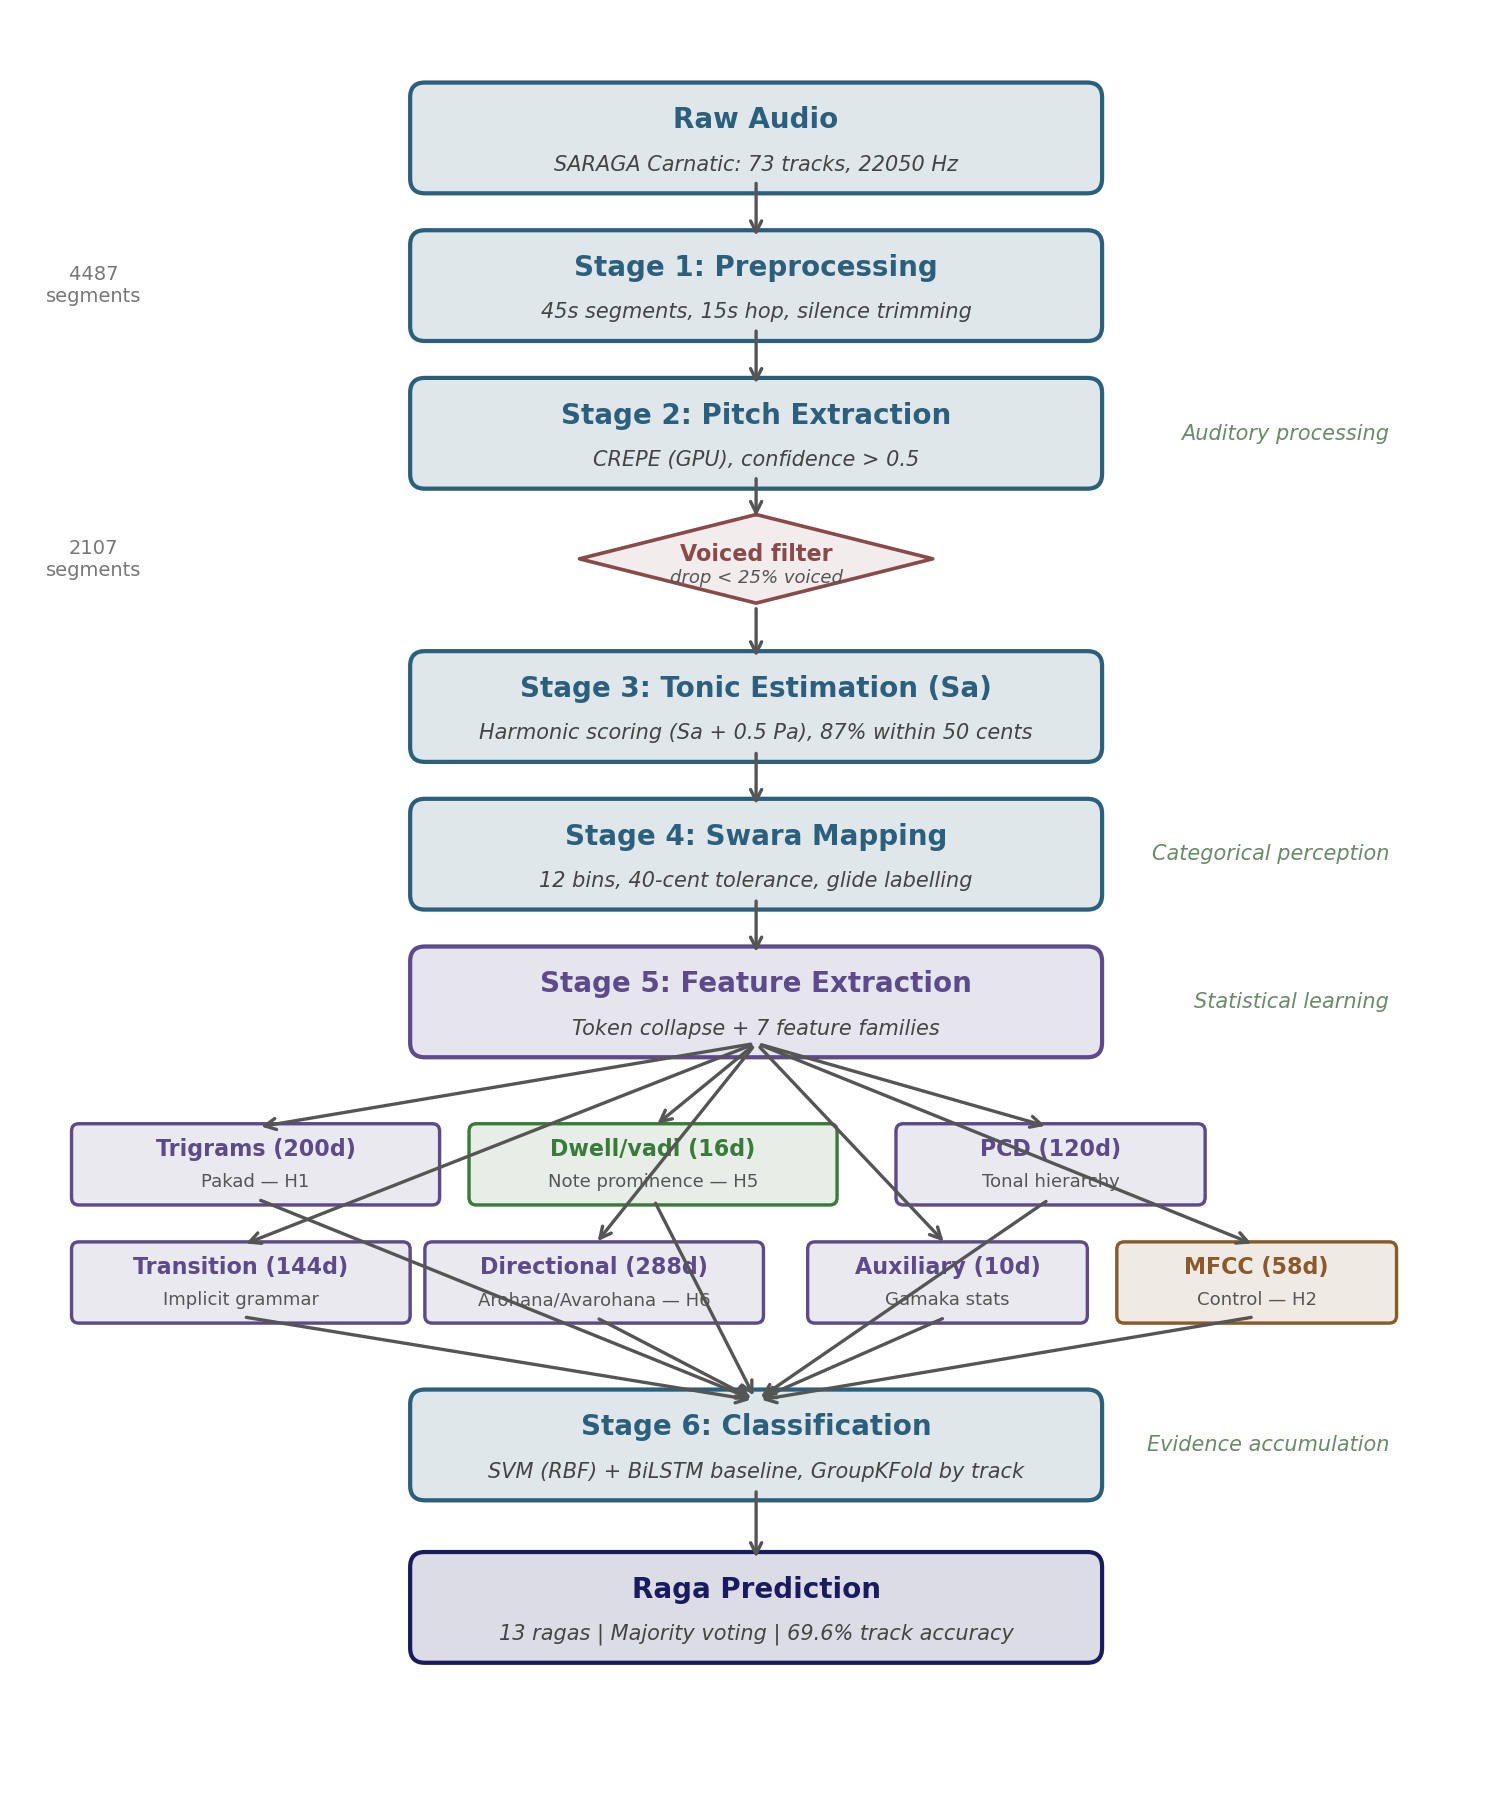
\includegraphics[width=0.8\textwidth]{outputs/figures/pipeline_diagram.png}
\caption{Six-stage pipeline architecture. Each stage mirrors a cognitive or musicological process. The seven feature families feed independently into the SVM classifier; Dwell/v\=adi (16d) achieves the best track-level weighted F1.}
\label{fig:app-pipeline}
\end{figure}

\subsection{Dataset Distribution}

\begin{figure}[H]
\centering
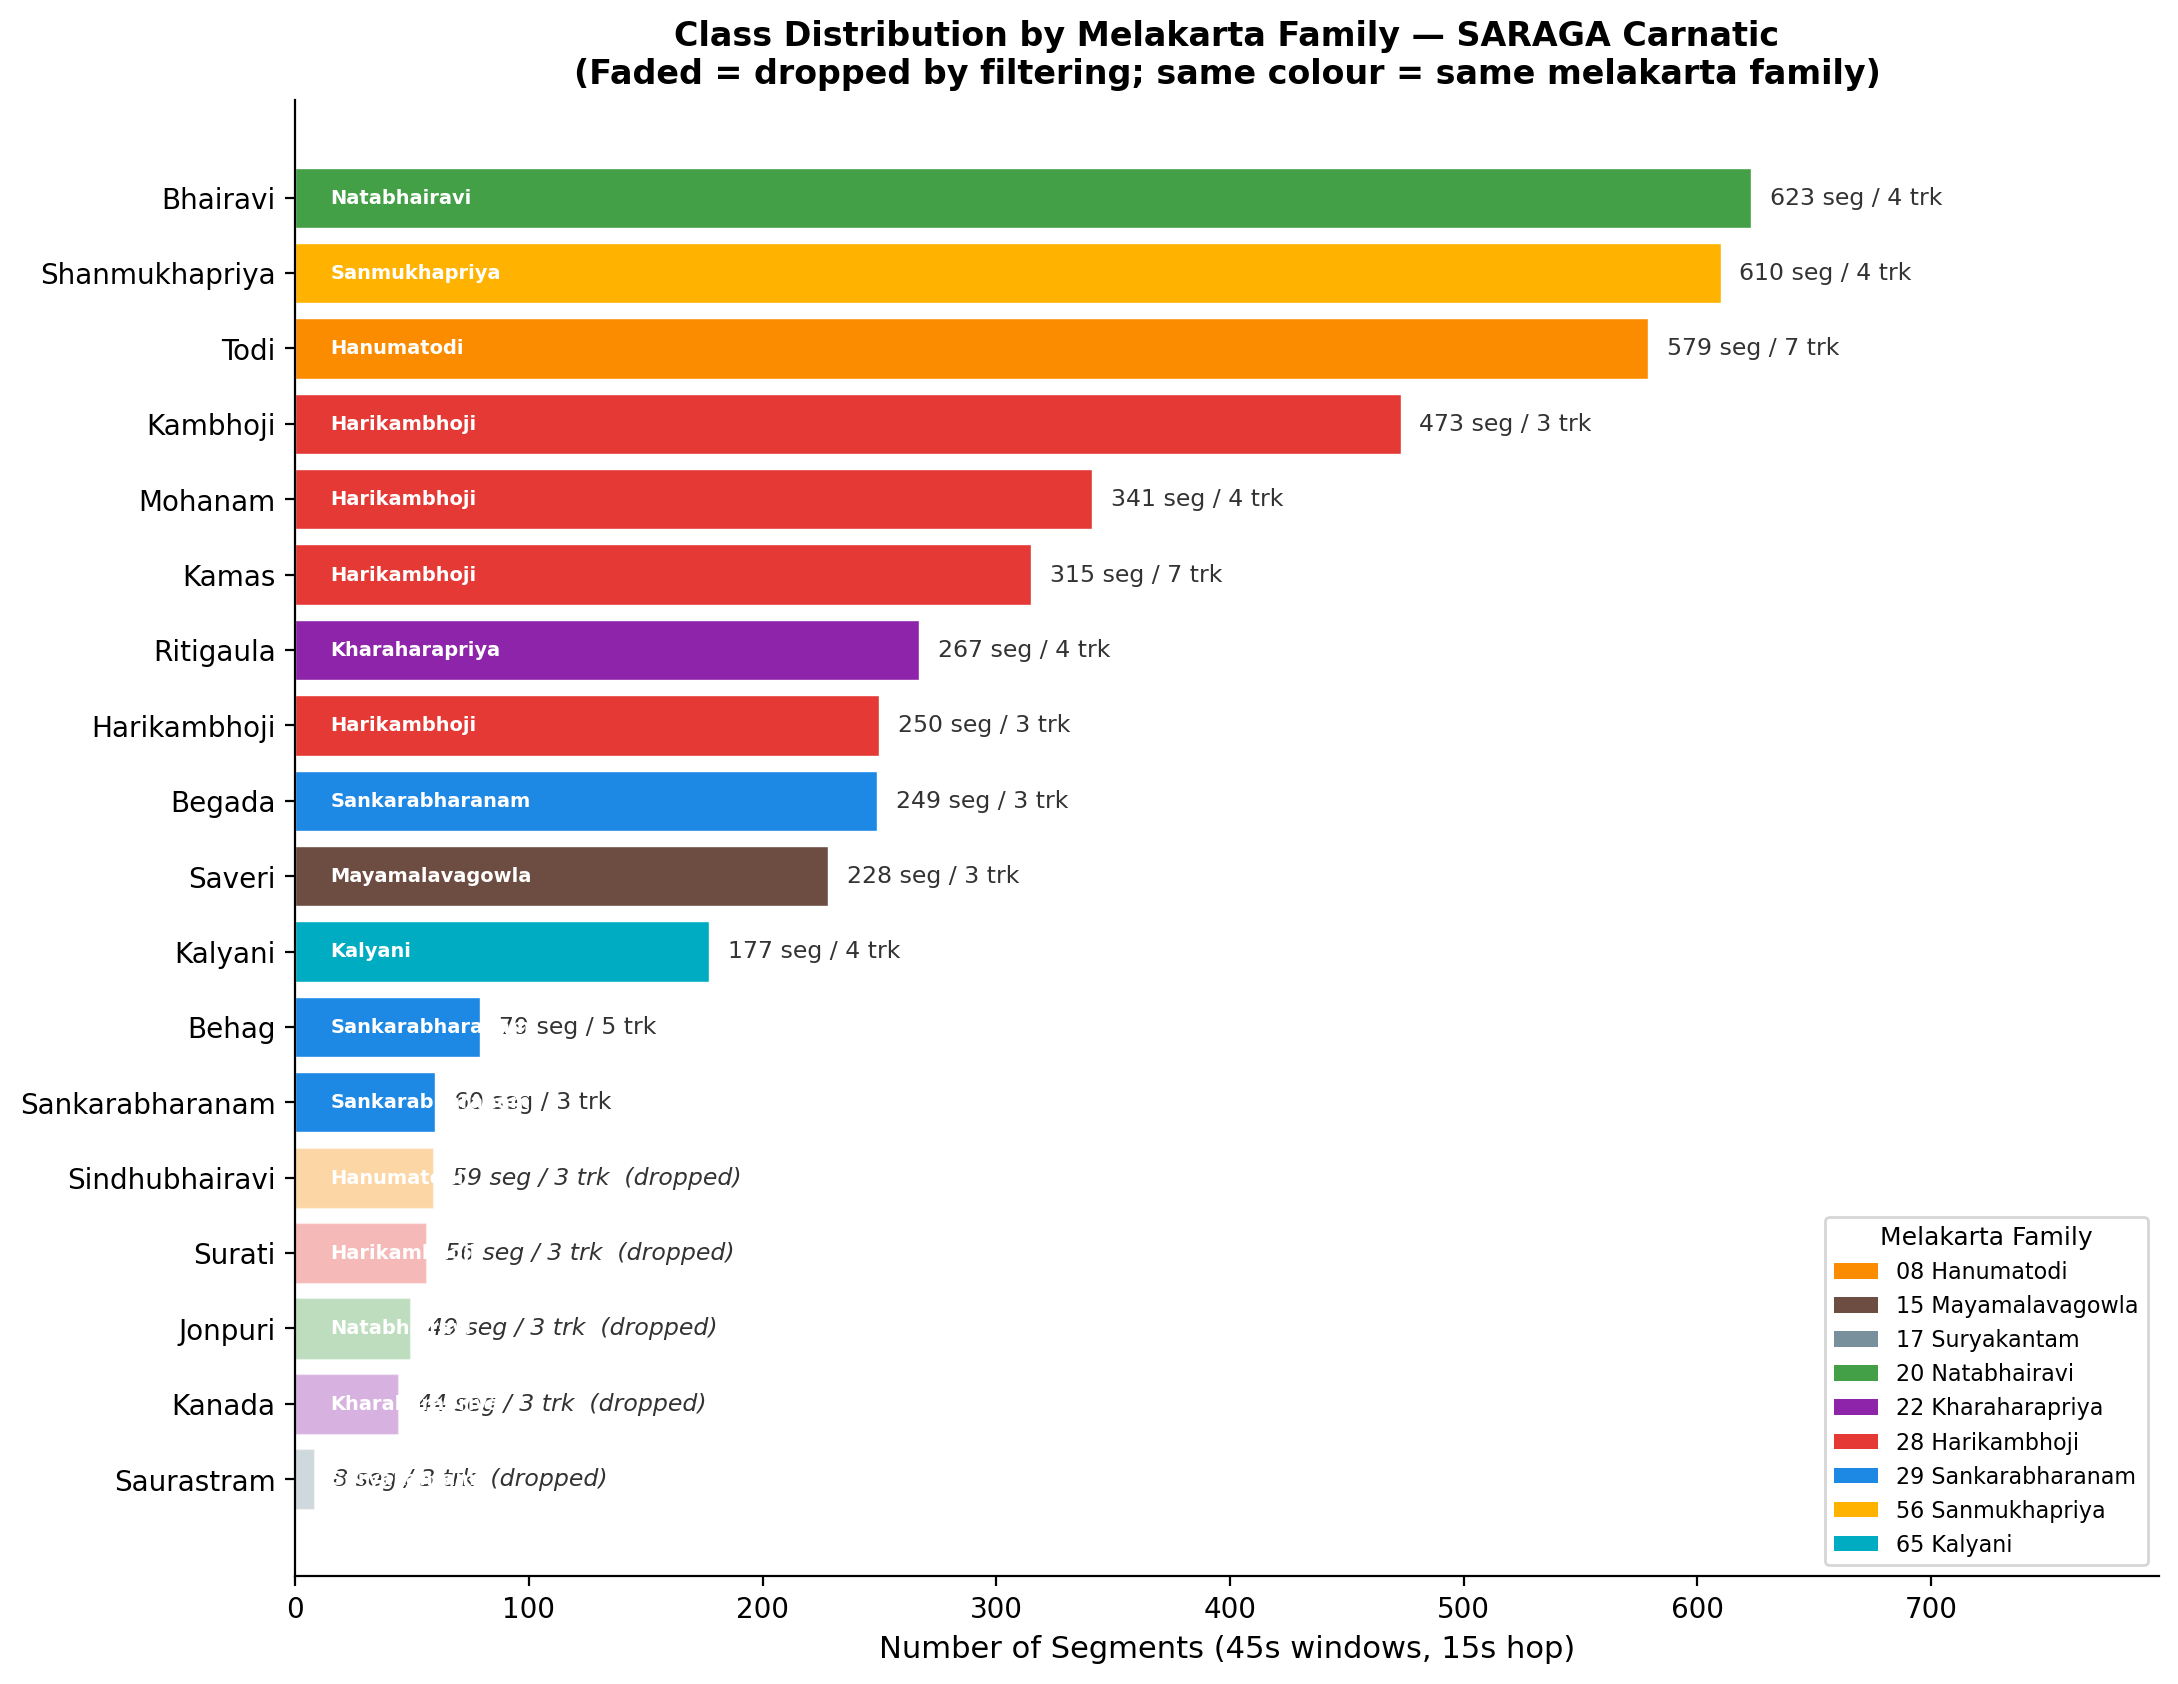
\includegraphics[width=0.85\textwidth]{outputs/figures/class_distribution.png}
\caption{Segment counts for all 18 \textit{ragas} in the SARAGA Carnatic subset, coloured by melakarta (parent scale) family. Faded bars indicate \textit{ragas} dropped during filtering ($<20$ segments after voiced-ratio and bad-tonic exclusion). The final evaluation set retains 13 \textit{ragas} across 46 tracks (1,648 segments) with a ${\sim}10{:}1$ imbalance between the largest (Bhairavi, 623) and smallest (\'Sankar\=abhara\d{n}a\d{m}, 60) classes. The five-member Harik\=ambh\=oji family (red) dominates both in membership and in within-family confusion (see \S\ref{sec:app-h4}).}
\label{fig:class-distribution}
\end{figure}

% ══════════════════════════════════════════════════════════
\section{Stage 2: Pitch Extraction}
% ══════════════════════════════════════════════════════════

Representative CREPE pitch extraction outputs showing the extracted F0 contour (top) and voicing confidence (bottom) for two different tracks. These plots verify that the pitch tracker captures continuous gamaka contours and correctly masks unvoiced regions.

\begin{figure}[H]
\centering
\begin{subfigure}[b]{0.48\textwidth}
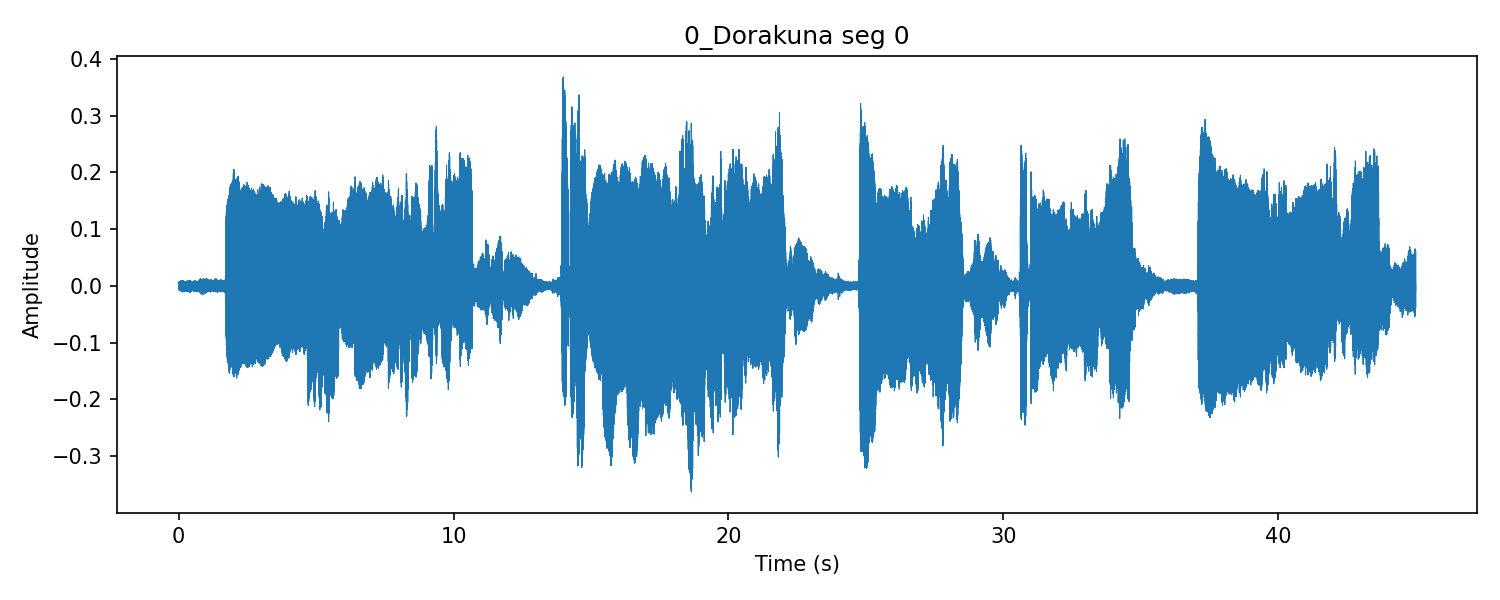
\includegraphics[width=\textwidth]{outputs/figures/pitch_debug/0_Dorakuna__00000.png}
\caption{Dorakuna, segment 0}
\end{subfigure}
\hfill
\begin{subfigure}[b]{0.48\textwidth}
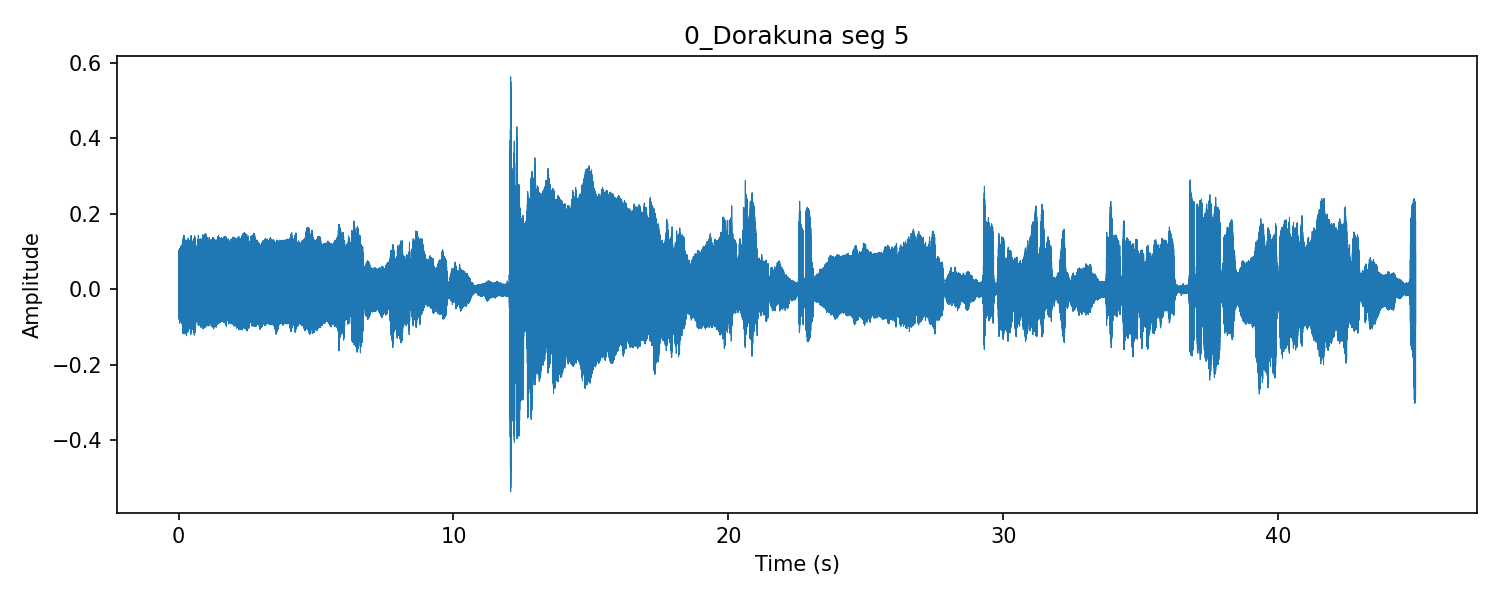
\includegraphics[width=\textwidth]{outputs/figures/pitch_debug/0_Dorakuna__00005.png}
\caption{Dorakuna, segment 5}
\end{subfigure}
\caption{Pitch extraction diagnostics for Dorakuna. The F0 contour (top) shows continuous pitch movement characteristic of Carnatic vocal gamaka. The confidence trace (bottom) cleanly separates voiced melodic regions from silence/percussion.}
\label{fig:app-pitch-debug-1}
\end{figure}

\begin{figure}[H]
\centering
\begin{subfigure}[b]{0.48\textwidth}
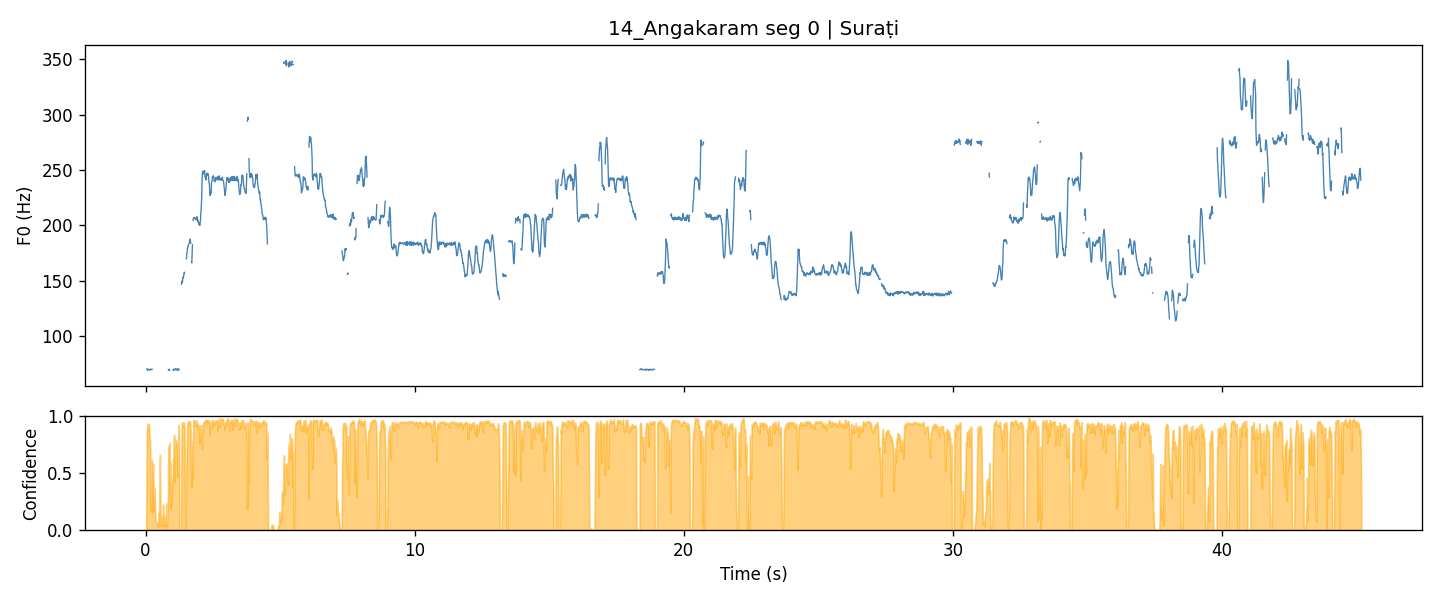
\includegraphics[width=\textwidth]{outputs/figures/pitch_debug/14_Angakaram__00000.png}
\caption{Angakaram, segment 0}
\end{subfigure}
\hfill
\begin{subfigure}[b]{0.48\textwidth}
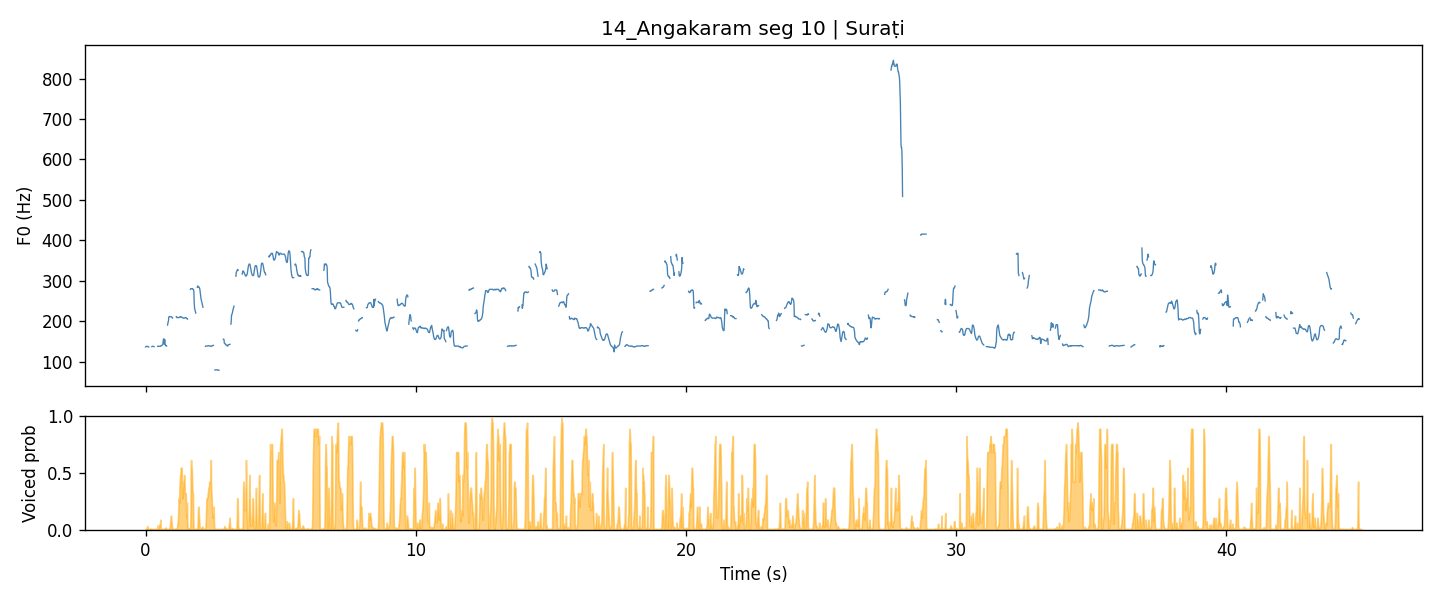
\includegraphics[width=\textwidth]{outputs/figures/pitch_debug/14_Angakaram__00010.png}
\caption{Angakaram, segment 10}
\end{subfigure}
\caption{Pitch extraction diagnostics for Angakaram. Note the wider pitch range and more frequent voicing gaps compared to Dorakuna, reflecting differences in performance style and accompanying instrumentation.}
\label{fig:app-pitch-debug-2}
\end{figure}

% ══════════════════════════════════════════════════════════
\section{Stage 3: Tonic Estimation}
% ══════════════════════════════════════════════════════════

\subsection{Baseline Results}

\begin{figure}[H]
\centering
\begin{subfigure}[b]{0.48\textwidth}
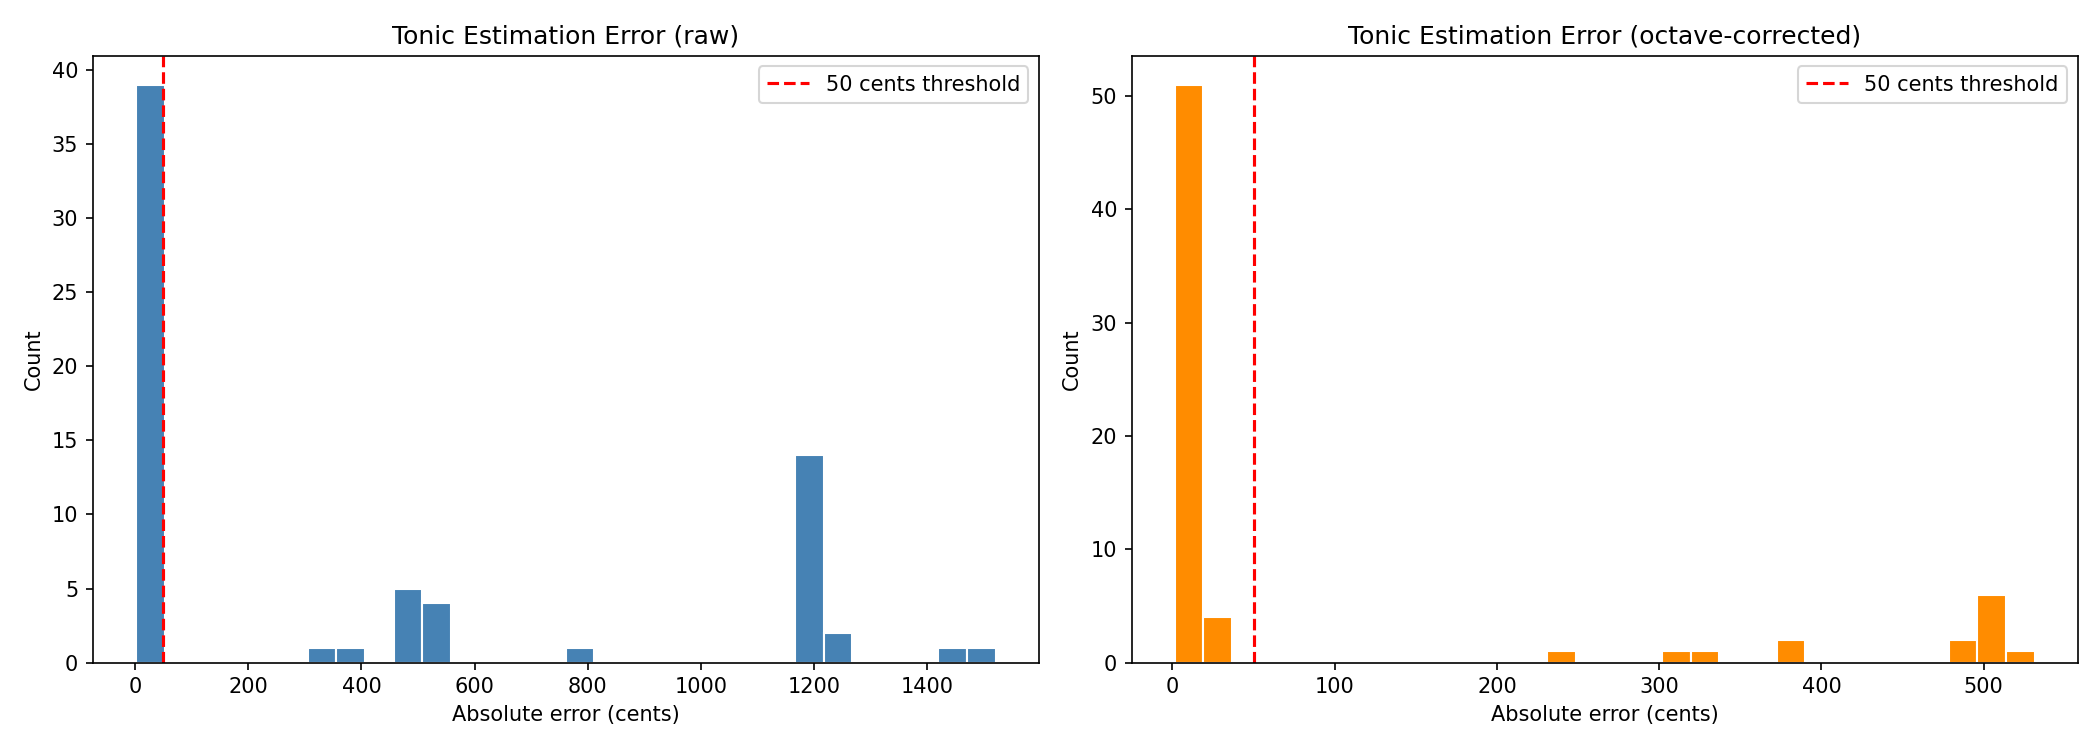
\includegraphics[width=\textwidth]{outputs/figures/tonic_validation/tonic_error_histogram_sa_mass.png}
\caption{Sa-mass scoring (79.7\% within 50 cents)}
\end{subfigure}
\hfill
\begin{subfigure}[b]{0.48\textwidth}
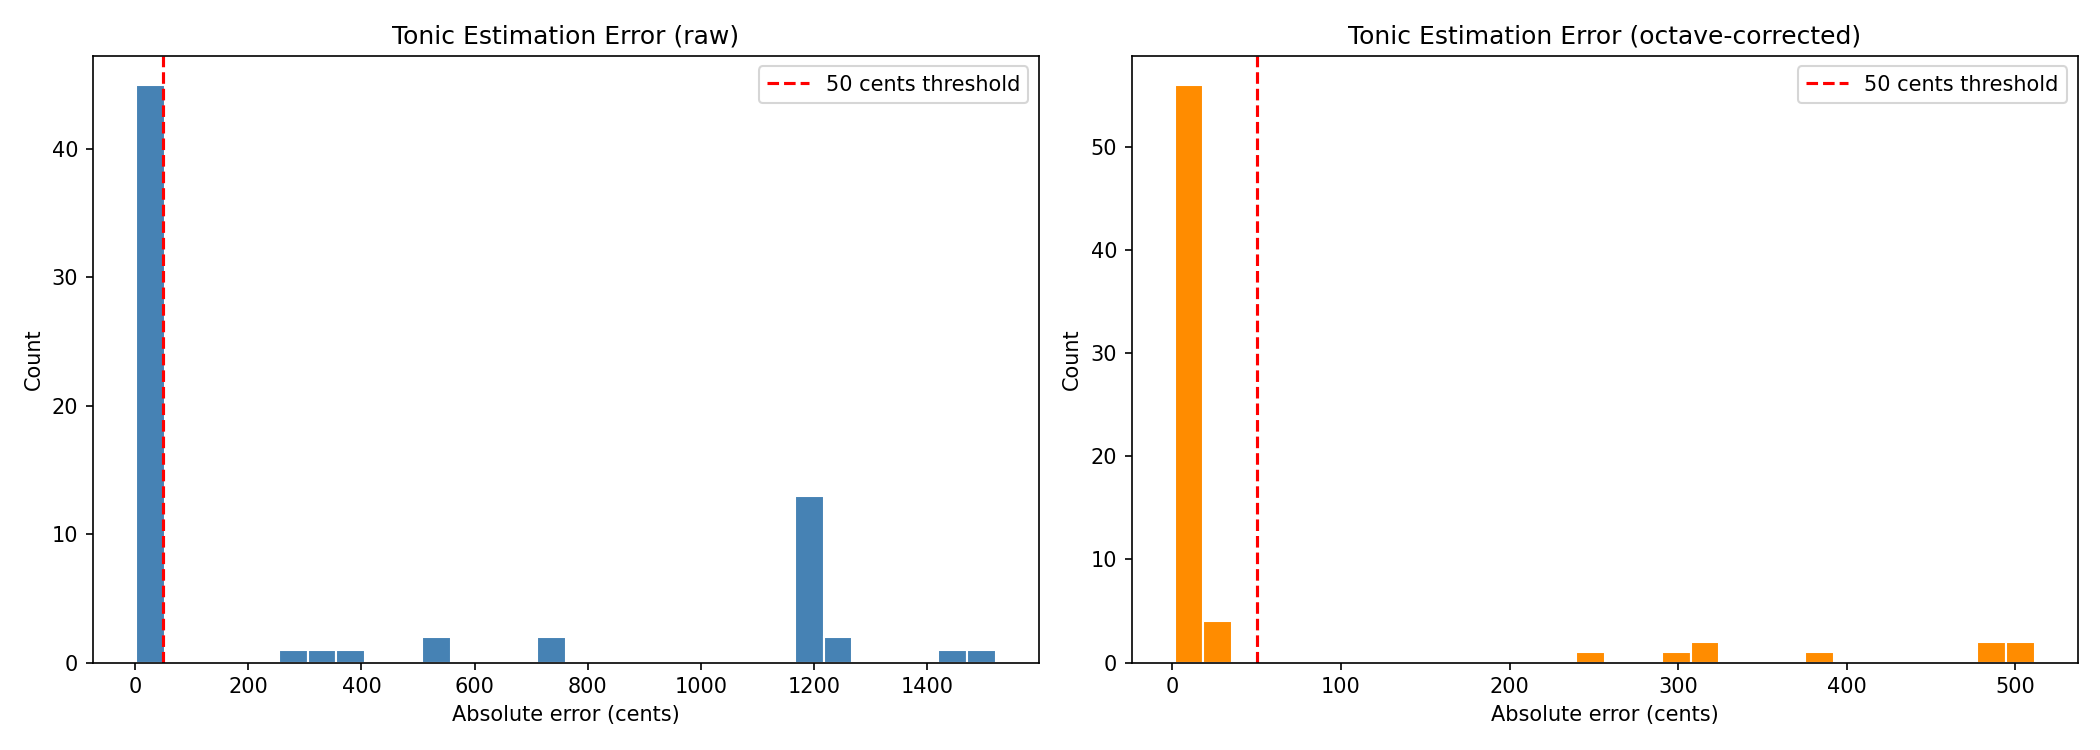
\includegraphics[width=\textwidth]{outputs/figures/tonic_validation/tonic_error_histogram_harmonic.png}
\caption{Harmonic scoring (87.0\% within 50 cents)}
\end{subfigure}
\caption{Tonic error histograms. Harmonic scoring produces a tighter distribution around zero cents error by exploiting the t\=anpura's Sa+Pa drone structure.}
\label{fig:app-tonic-histograms}
\end{figure}

\begin{figure}[H]
\centering
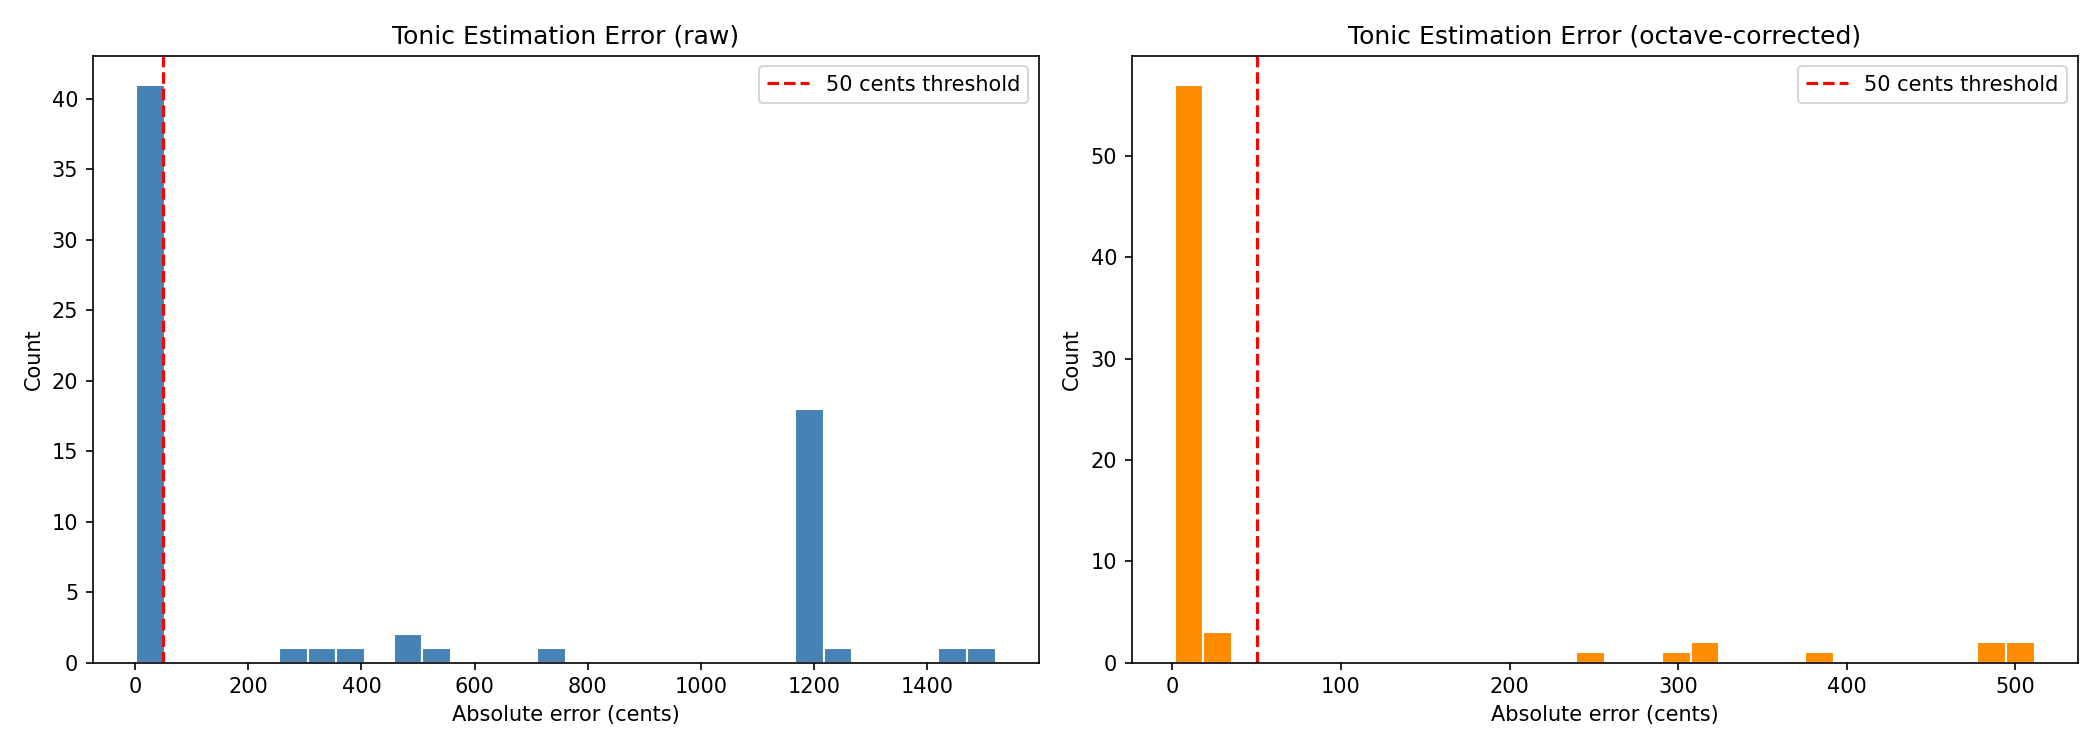
\includegraphics[width=0.75\textwidth]{outputs/figures/tonic_validation/tonic_error_histogram_smoothed_harmonic.png}
\caption{Smoothed harmonic scoring ($\sigma=2$ bins): reduces narrow-peak sensitivity but does not improve overall accuracy. More octave errors than unsmoothed harmonic.}
\label{fig:app-tonic-smoothed}
\end{figure}

\begin{figure}[H]
\centering
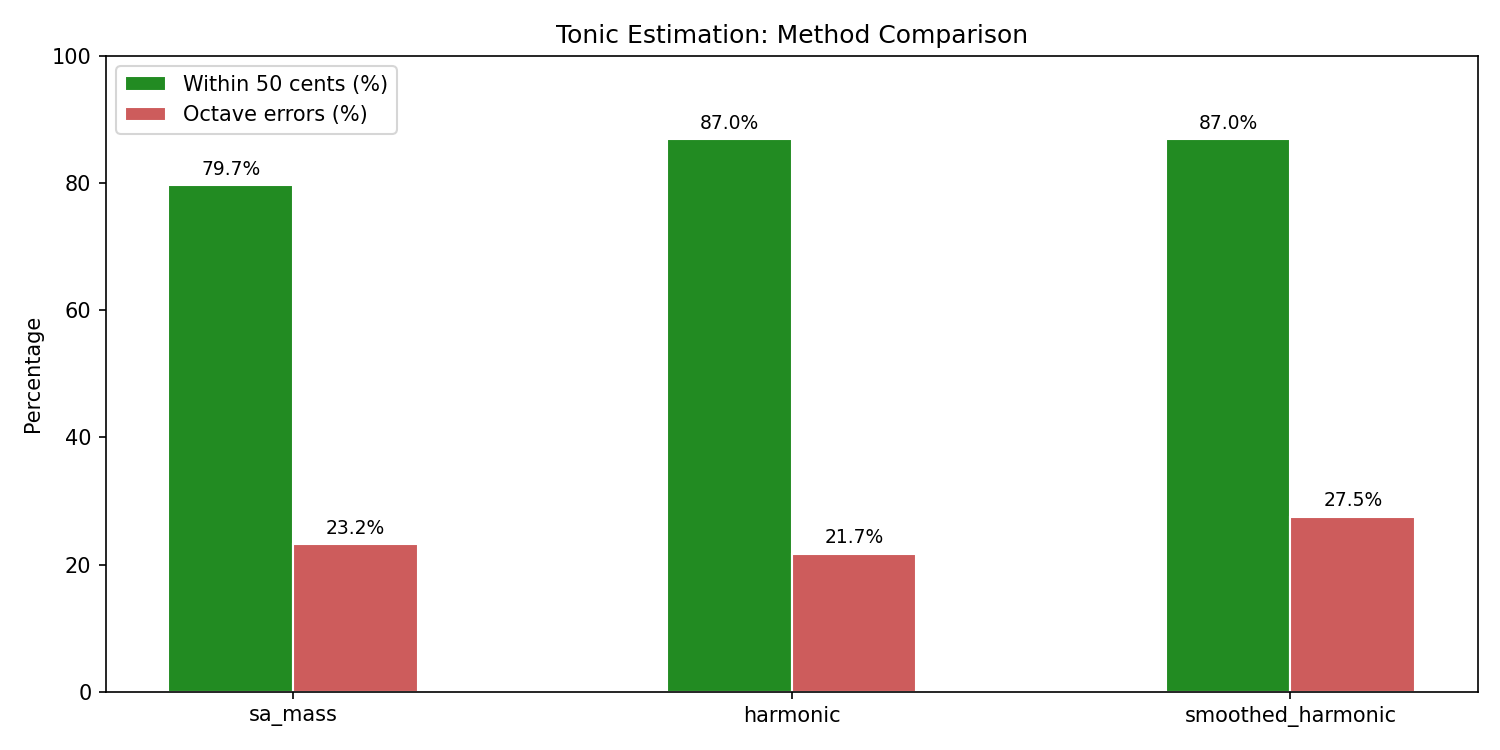
\includegraphics[width=0.75\textwidth]{outputs/figures/tonic_validation/tonic_method_comparison.png}
\caption{Head-to-head comparison of all three tonic scoring methods. Harmonic scoring achieves the highest within-50-cents accuracy (87.0\%) with the fewest octave errors, confirming that the t\=anpura's Sa+Pa drone structure provides a reliable perceptual anchor for tonic estimation.}
\label{fig:app-tonic-comparison}
\end{figure}

\subsection{Tonic Experiments (Including Failed)}

The following experiments attempted to improve tonic estimation beyond the harmonic baseline.

\begin{itemize}
  \item \textbf{Harmonic triad scoring}: Extended Sa+Pa to Sa+Ma+Pa with a Pa$>$Sa penalty. Marginal improvement, confirming that the simpler Sa+Pa scoring already captures the dominant cue.
  \item \textbf{Ensemble voting}: Combined multiple scoring methods via weighted voting. Did not exceed the best single method.
  \item \textbf{Segment-level voting}: Per-segment tonic estimates aggregated via octave-invariant majority vote. Reduced outlier sensitivity but did not improve median accuracy.
  \item \textbf{Swara-validated tonic}: Used swara distribution quality as a secondary validation signal. Circular dependency (swara mapping requires a tonic) limited effectiveness.
\end{itemize}

\begin{figure}[H]
\centering
\begin{subfigure}[b]{0.48\textwidth}
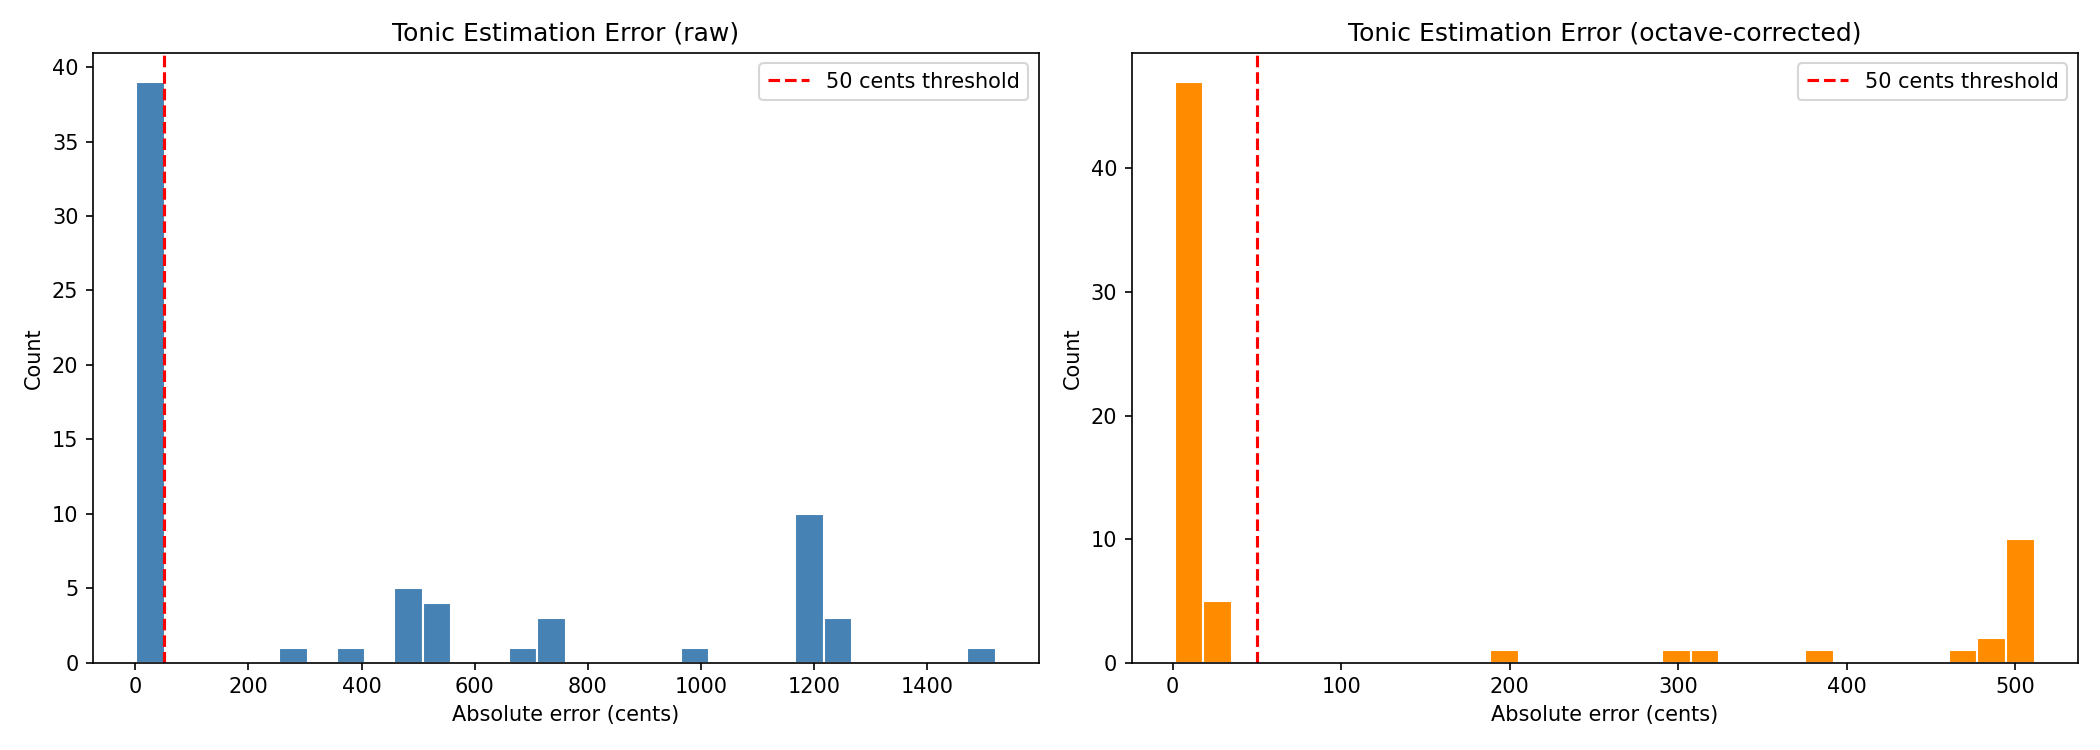
\includegraphics[width=\textwidth]{outputs/figures/tonic_validation/tonic_error_histogram_triad.png}
\caption{Triad scoring error distribution}
\end{subfigure}
\hfill
\begin{subfigure}[b]{0.48\textwidth}
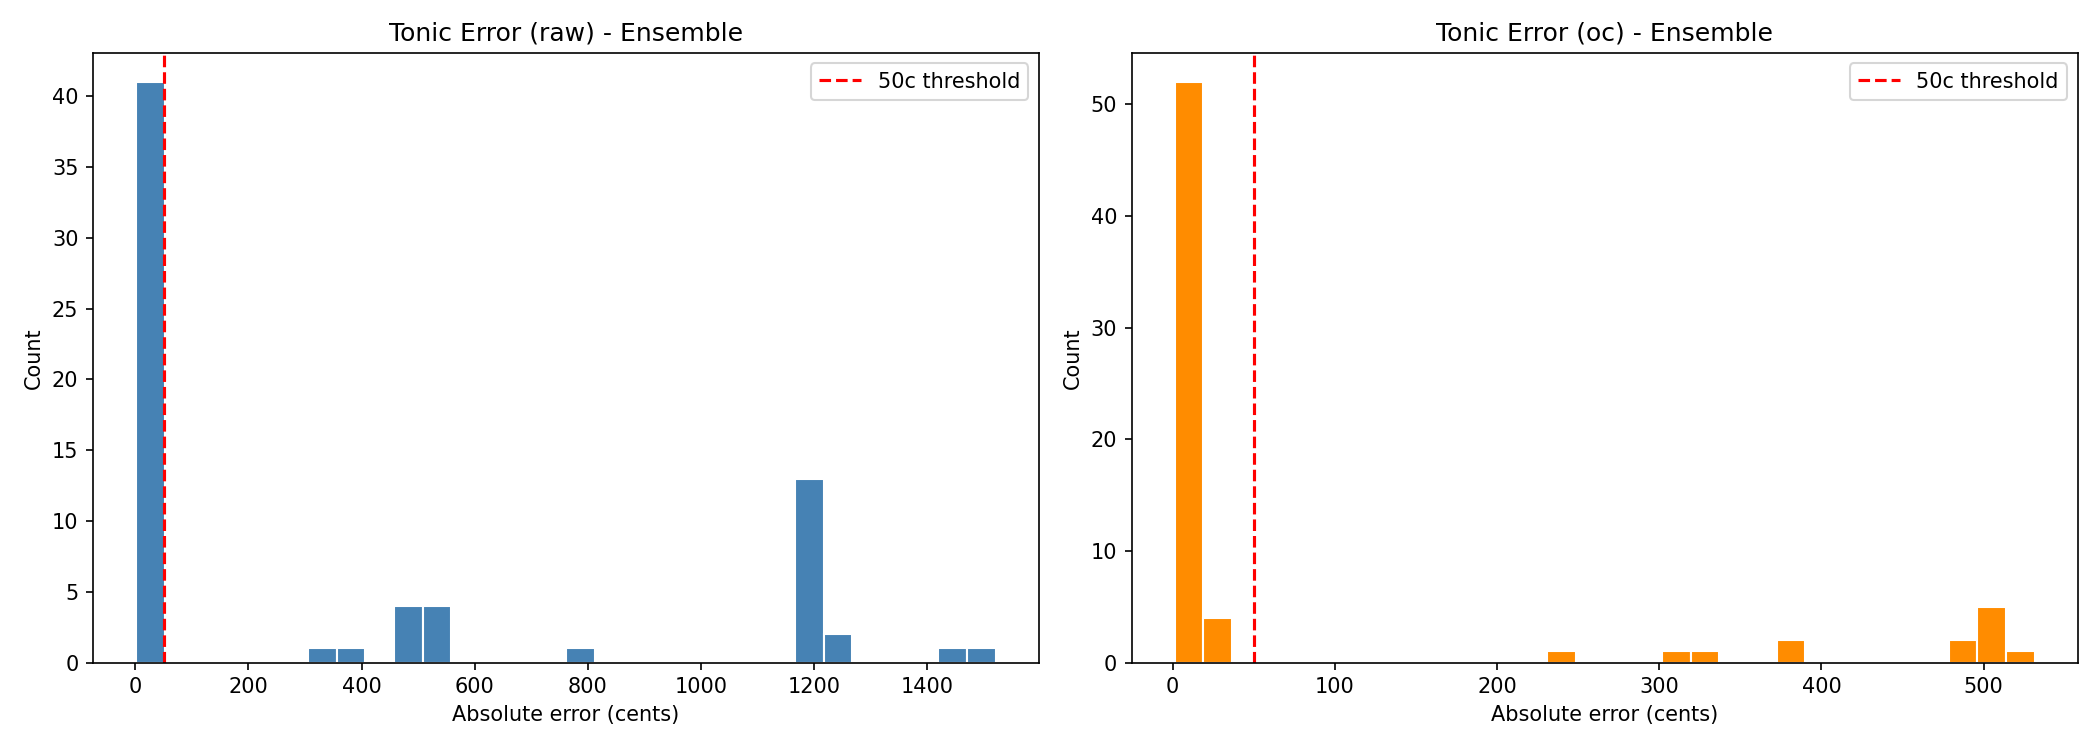
\includegraphics[width=\textwidth]{outputs/figures/tonic_validation/tonic_error_histogram_ensemble.png}
\caption{Ensemble voting error distribution}
\end{subfigure}
\caption{Tonic experiment error histograms. Neither the triad extension nor the ensemble approach substantially improved over the harmonic baseline (87.0\% within 50 cents).}
\label{fig:app-tonic-experiments}
\end{figure}

\begin{figure}[H]
\centering
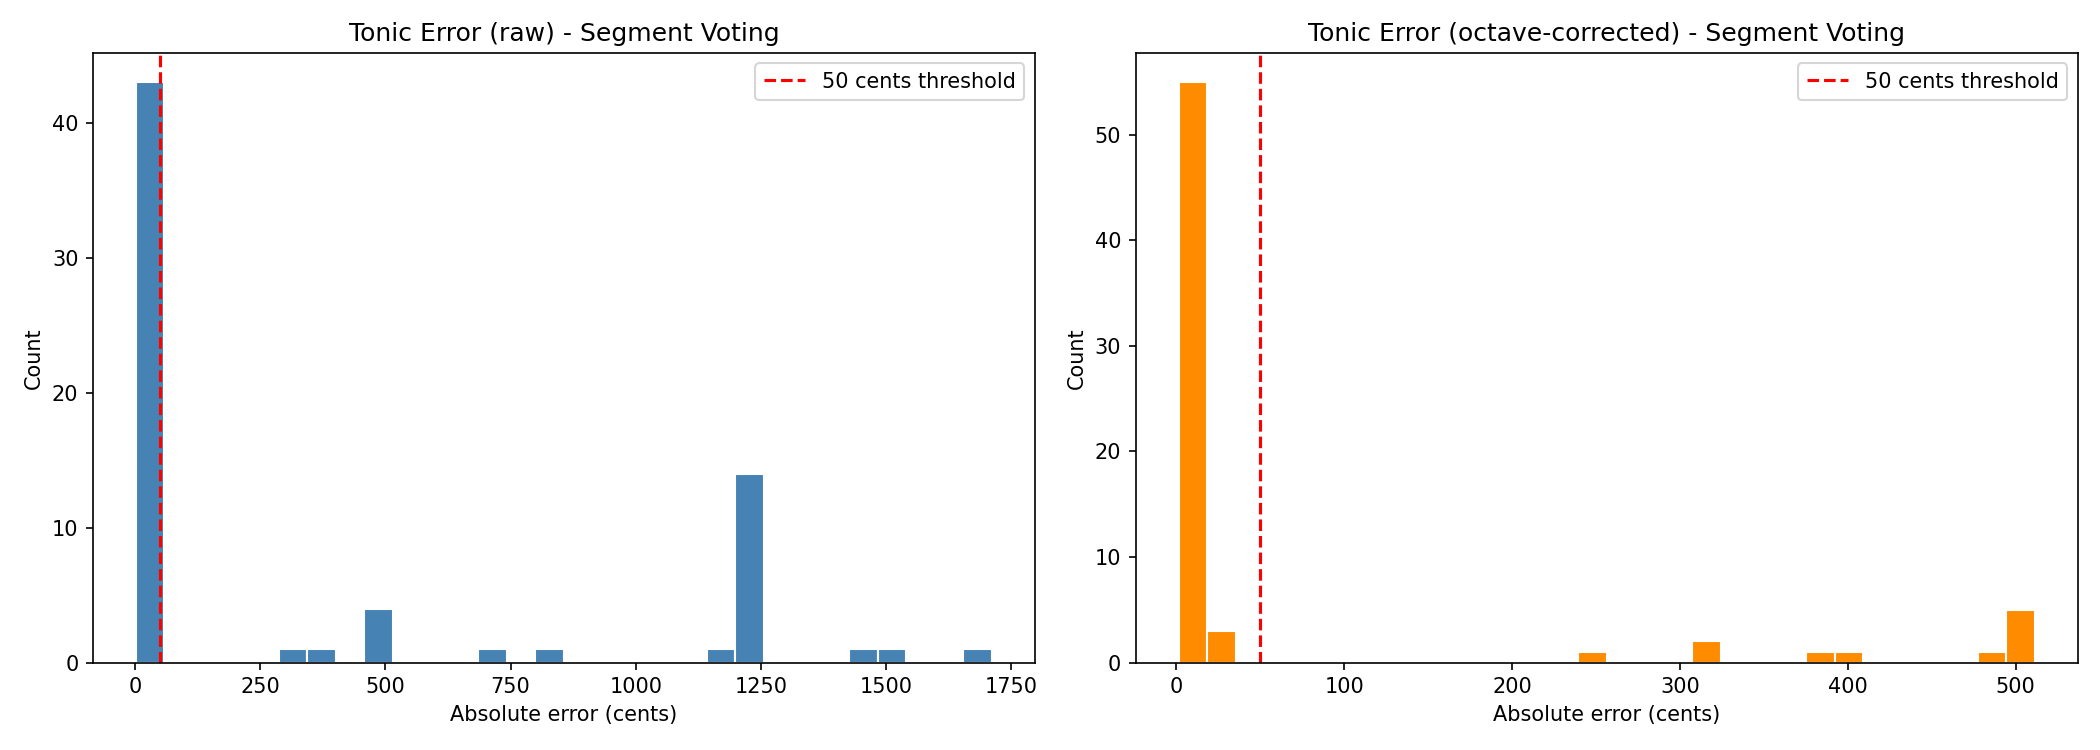
\includegraphics[width=0.75\textwidth]{outputs/figures/tonic_validation/tonic_error_histogram_segment_voting.png}
\caption{Segment-level voting tonic estimation. Per-segment estimates are aggregated via octave-invariant majority vote. Reduces outlier sensitivity but does not improve median accuracy over the track-level harmonic baseline.}
\label{fig:app-tonic-segment-voting}
\end{figure}

% ══════════════════════════════════════════════════════════
\section{Stage 4: Swara Mapping}
% ══════════════════════════════════════════════════════════

Swara mapping overlays the discrete swara labels (bottom, colour-coded) onto the continuous pitch contour in cents (top). These plots verify that the 40-cent tolerance correctly assigns swaras while labelling inter-note gamaka movement as ``glide.''

\begin{figure}[H]
\centering
\begin{subfigure}[b]{0.48\textwidth}
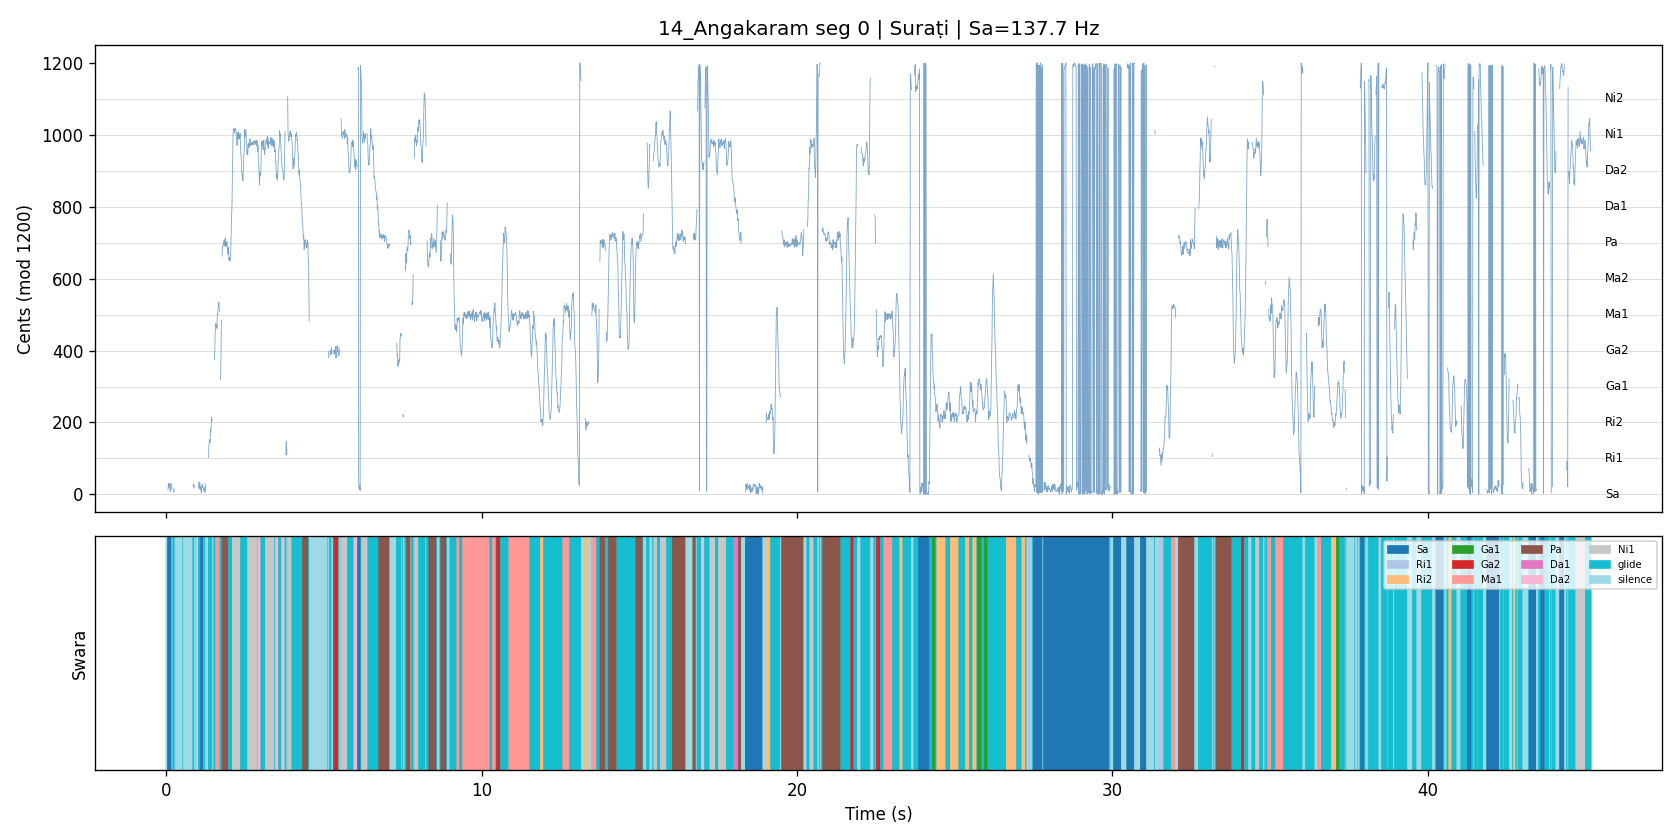
\includegraphics[width=\textwidth]{outputs/figures/swara_debug/14_Angakaram__00000_swara.png}
\caption{Angakaram, segment 0}
\end{subfigure}
\hfill
\begin{subfigure}[b]{0.48\textwidth}
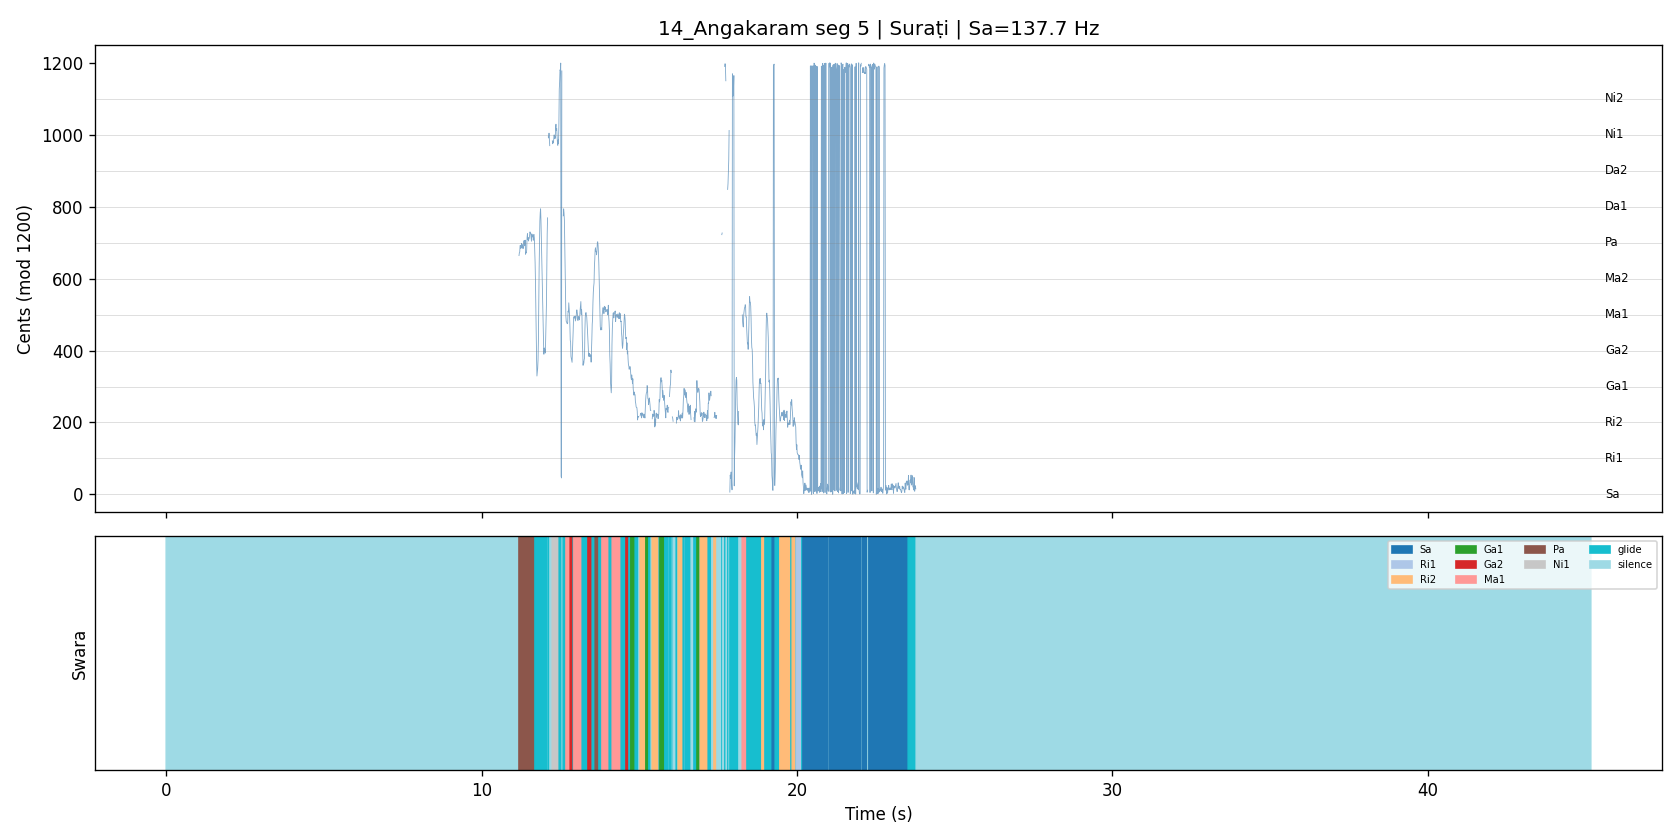
\includegraphics[width=\textwidth]{outputs/figures/swara_debug/14_Angakaram__00005_swara.png}
\caption{Angakaram, segment 5}
\end{subfigure}
\caption{Swara mapping diagnostics. Top: pitch contour in cents (mod 1200) with horizontal lines at each swara bin. Bottom: colour-coded swara labels. ``Glide'' regions (visible between discrete swara assignments) correspond to ornamental gamaka movement, comprising ${\sim}28\%$ of voiced frames across the dataset.}
\label{fig:app-swara-debug-1}
\end{figure}

\begin{figure}[H]
\centering
\begin{subfigure}[b]{0.48\textwidth}
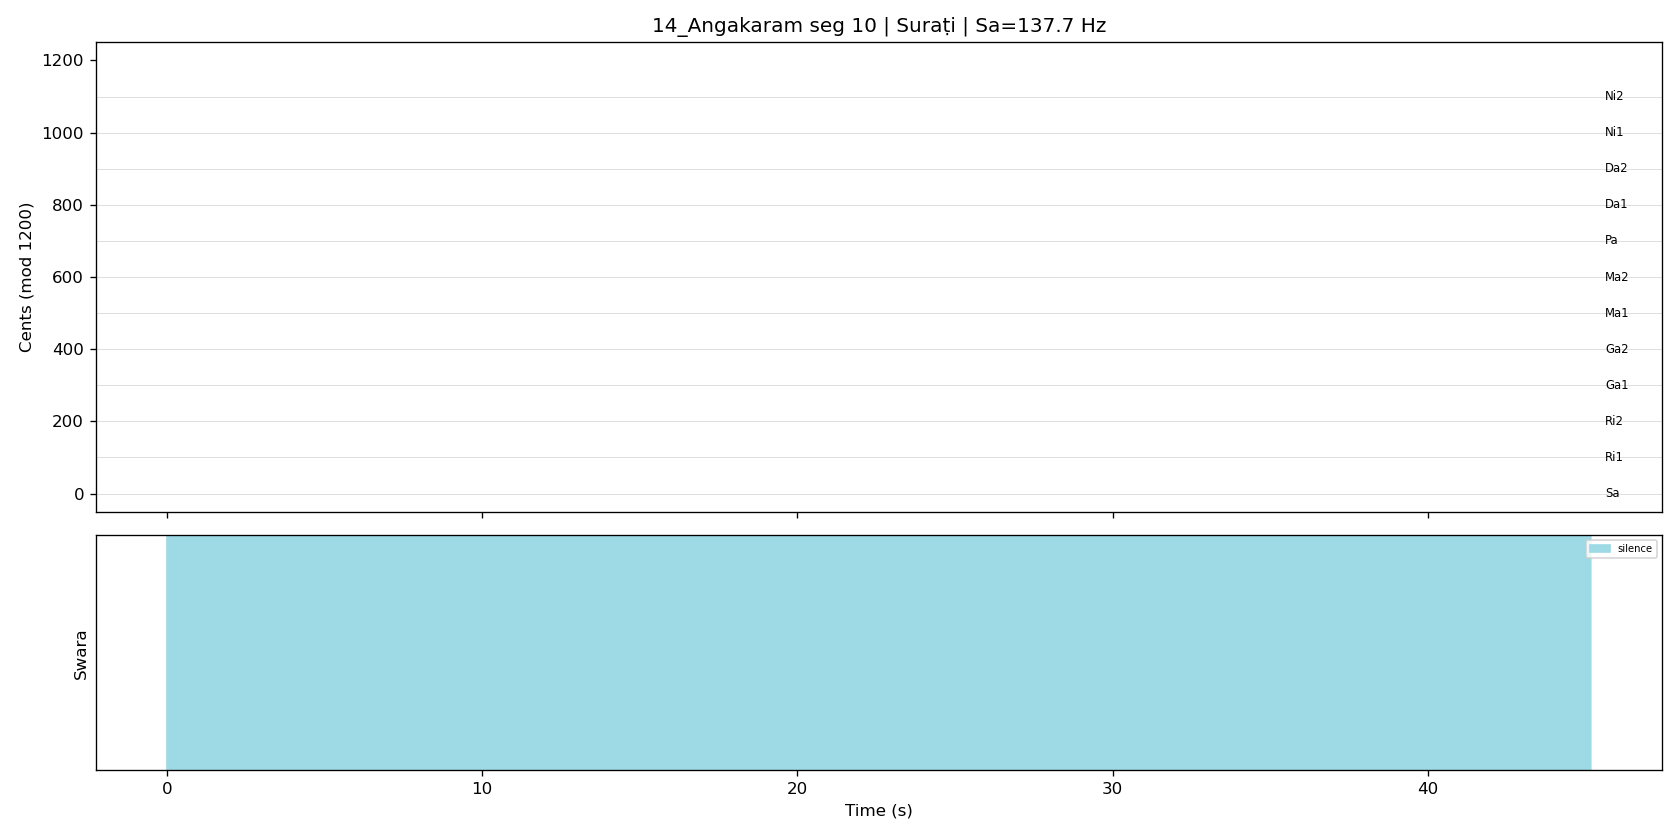
\includegraphics[width=\textwidth]{outputs/figures/swara_debug/14_Angakaram__00010_swara.png}
\caption{Angakaram, segment 10}
\end{subfigure}
\hfill
\begin{subfigure}[b]{0.48\textwidth}
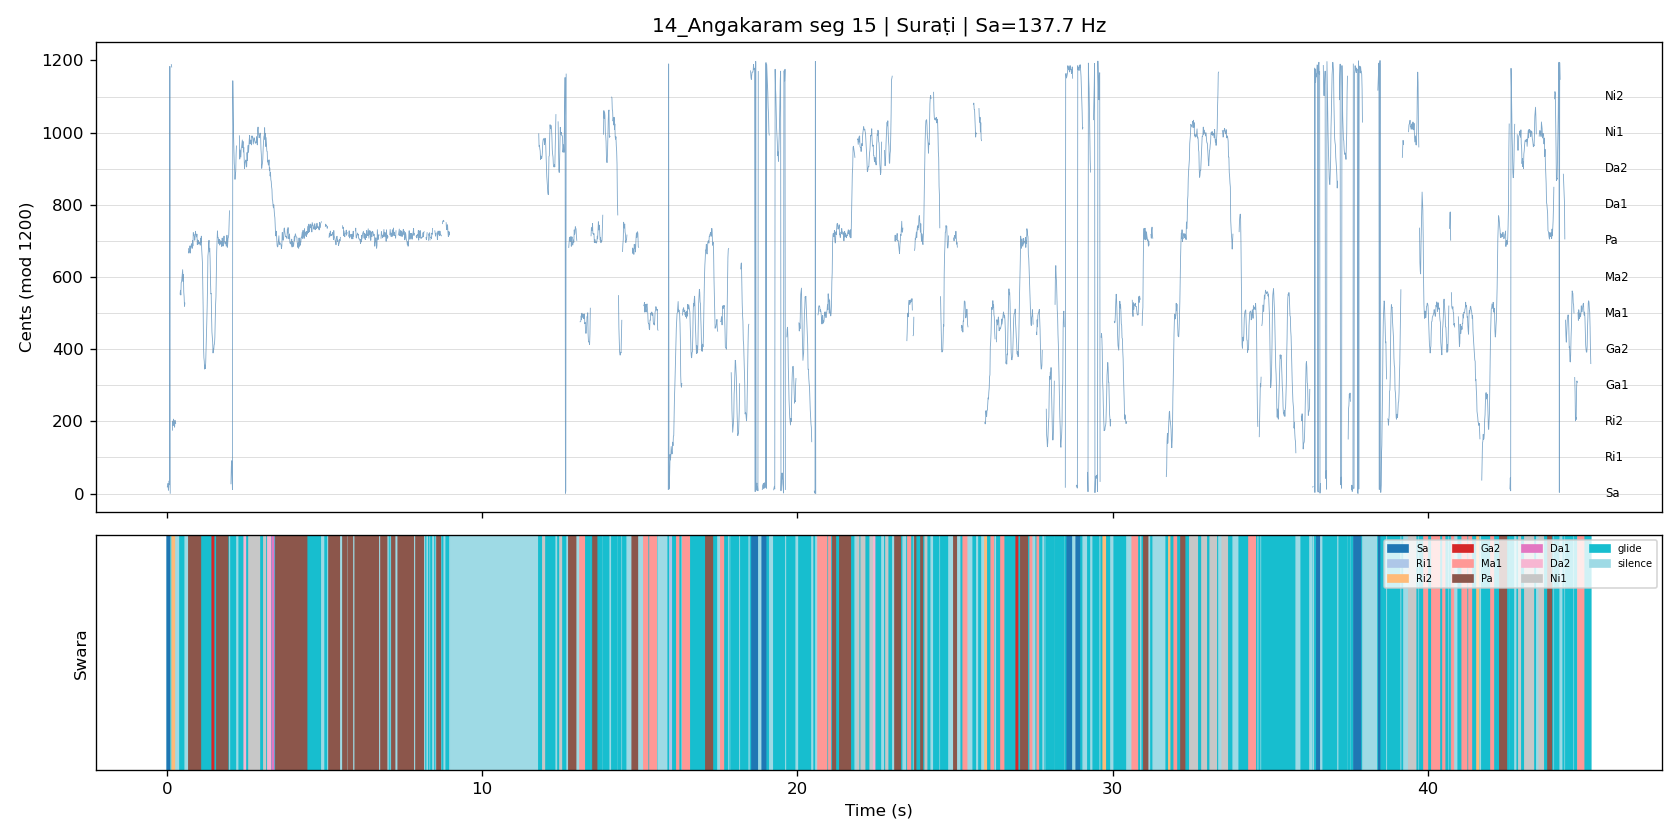
\includegraphics[width=\textwidth]{outputs/figures/swara_debug/14_Angakaram__00015_swara.png}
\caption{Angakaram, segment 15}
\end{subfigure}
\caption{Additional swara mapping examples. The minimum-duration filter (100\,ms) suppresses rapid label flickering from pitch estimation noise, visible as consolidated colour blocks rather than single-frame assignments.}
\label{fig:app-swara-debug-2}
\end{figure}

% ══════════════════════════════════════════════════════════
\section{Stage 5: Feature Extraction}
% ══════════════════════════════════════════════════════════

These figures show per-\textit{raga} pitch class distributions (120-bin histograms), swara transition matrices ($12\times12$ heatmaps), and directional features. They demonstrate that \textit{ragas} with distinctive profiles classify well, while Harik\=ambh\=oji-family \textit{ragas} with overlapping profiles are confused.

\subsection{Pitch Class Distributions}

\begin{figure}[H]
\centering
\begin{subfigure}[b]{0.48\textwidth}
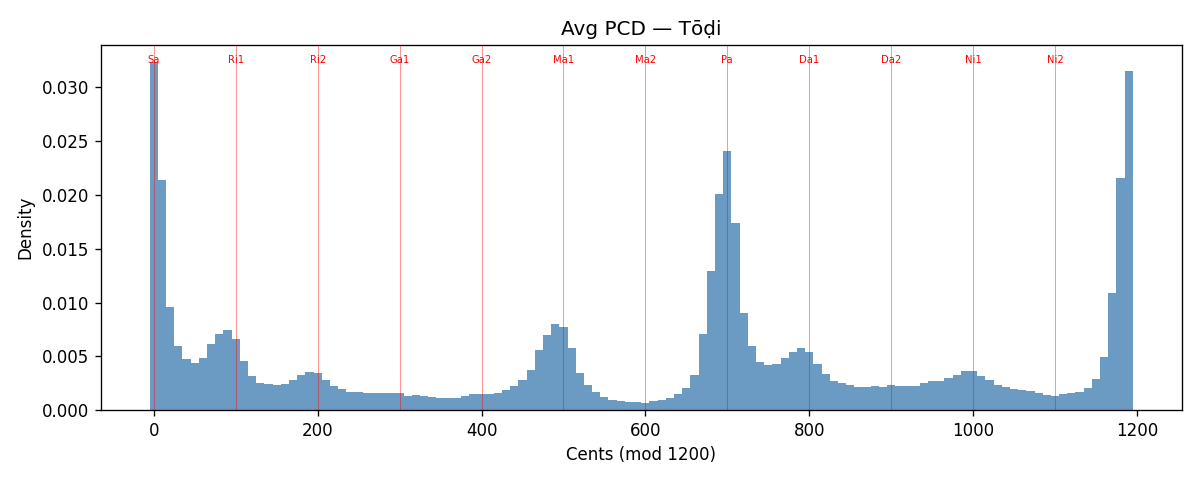
\includegraphics[width=\textwidth]{outputs/figures/features/pcd_Todi.png}
\caption{T\=o\d{d}i (0.86 F1) --- unique intervallic signature}
\end{subfigure}
\hfill
\begin{subfigure}[b]{0.48\textwidth}
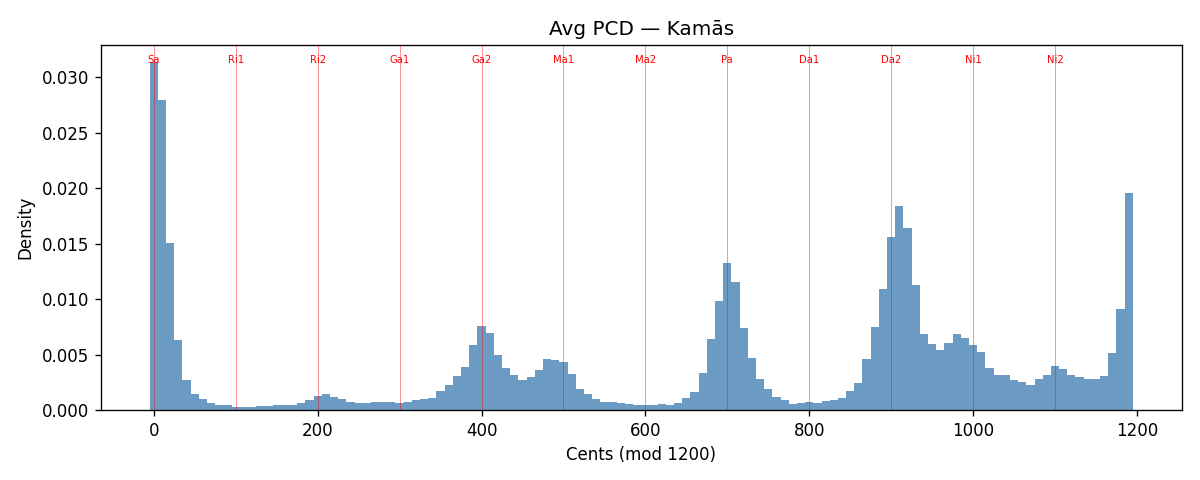
\includegraphics[width=\textwidth]{outputs/figures/features/pcd_Kamas.png}
\caption{Kam\=as (0.36 F1) --- overlaps with Harik\=ambh\=oji family}
\end{subfigure}
\caption{Pitch class distributions. T\=o\d{d}i's distinctive Ri1--Ga1 peaks explain its high classification performance. Kam\=as's PCD is nearly identical to its parent melakarta, explaining the family confusion.}
\label{fig:app-pcd}
\end{figure}

\begin{figure}[H]
\centering
\begin{subfigure}[b]{0.48\textwidth}
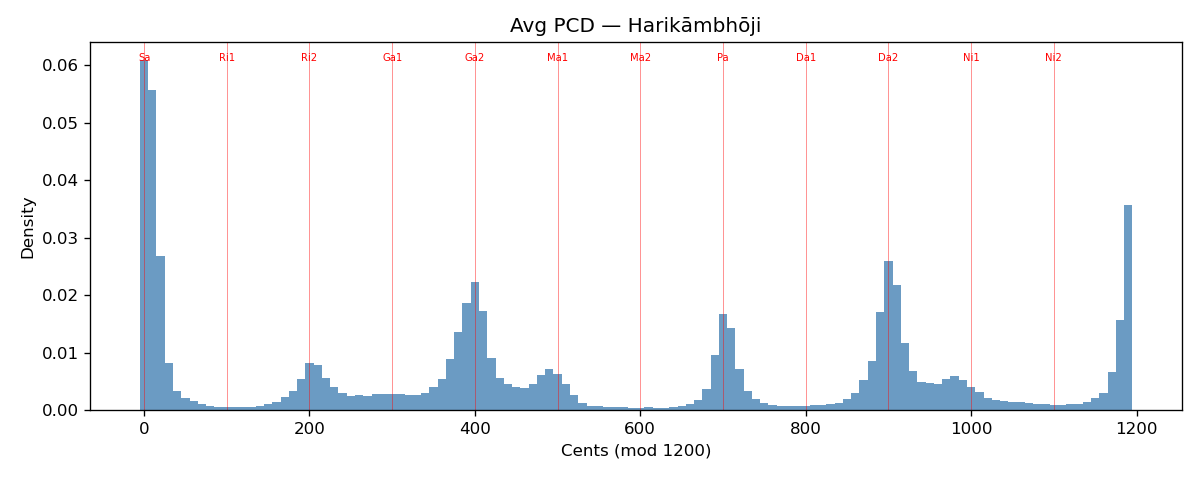
\includegraphics[width=\textwidth]{outputs/figures/features/pcd_Harikambhoji.png}
\caption{Harik\=ambh\=oji (parent, 0\% F1)}
\end{subfigure}
\hfill
\begin{subfigure}[b]{0.48\textwidth}
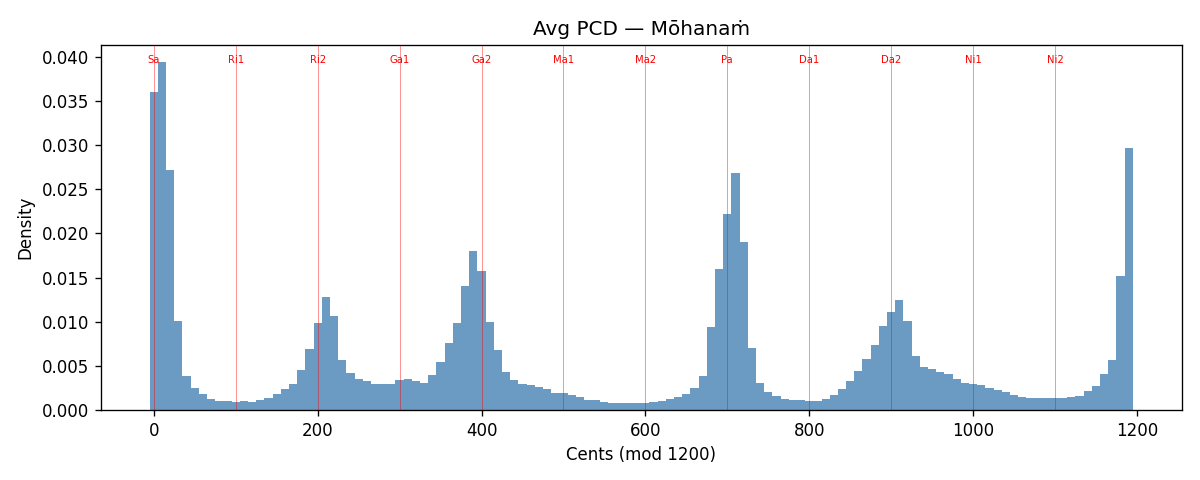
\includegraphics[width=\textwidth]{outputs/figures/features/pcd_Mohanam.png}
\caption{M\=ohana\.{m} (pentatonic, janya of Harik\=ambh\=oji)}
\end{subfigure}
\caption{Harik\=ambh\=oji (parent) vs M\=ohana\.{m} (child). The parent's PCD is a superset of the child's --- every peak in M\=ohana\.{m} also appears in Harik\=ambh\=oji, explaining the family confusion that drives H4. M\=ohana\.{m}'s identity lies in what is \textit{absent} (no Ma, no Ni), but our features encode presence, not absence.}
\label{fig:app-pcd-2}
\end{figure}

\subsection{Transition Matrices}

\begin{figure}[H]
\centering
\begin{subfigure}[b]{0.48\textwidth}
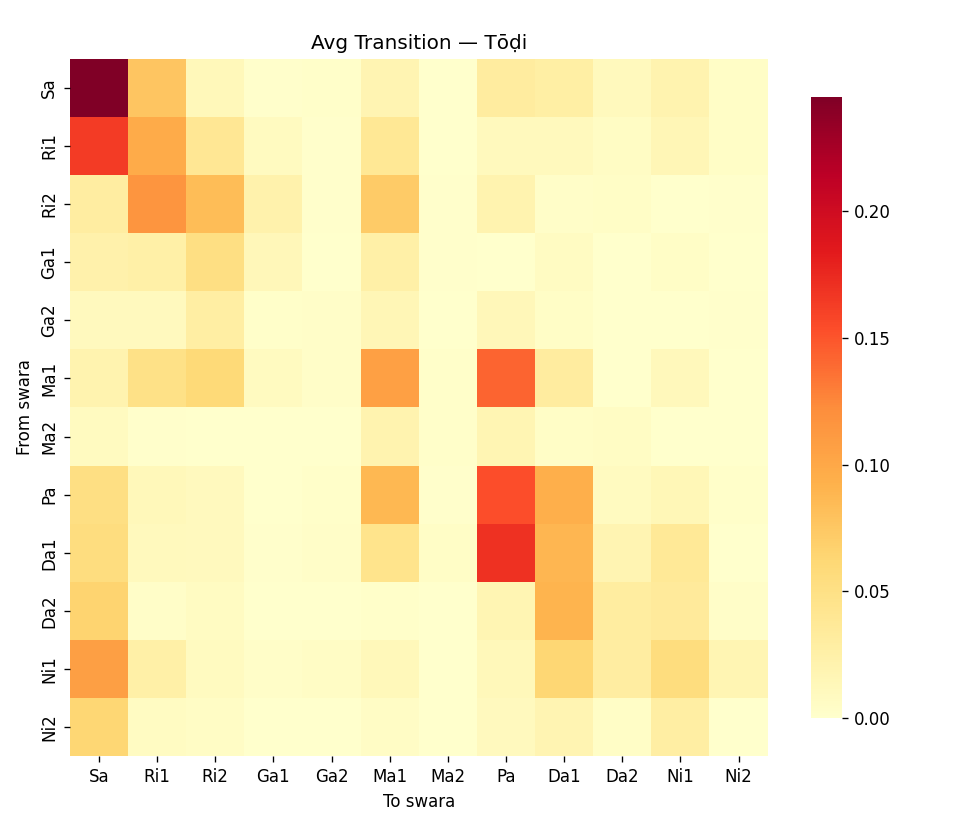
\includegraphics[width=\textwidth]{outputs/figures/features/transition_Todi.png}
\caption{T\=o\d{d}i --- concentrated transitions}
\end{subfigure}
\hfill
\begin{subfigure}[b]{0.48\textwidth}
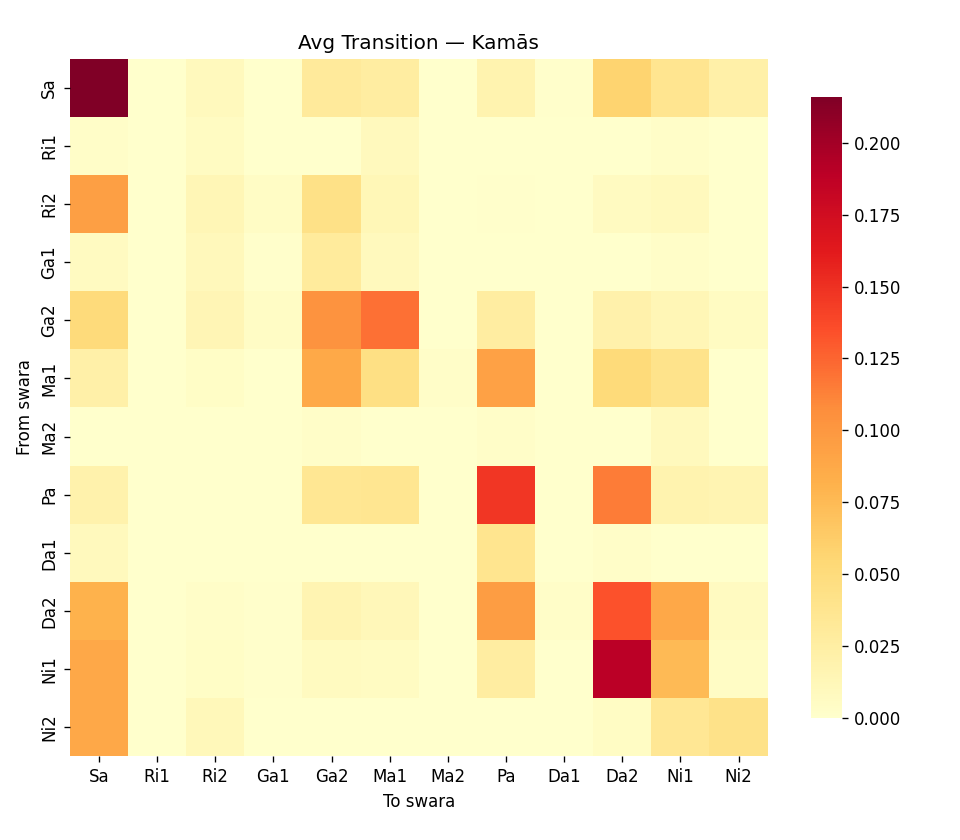
\includegraphics[width=\textwidth]{outputs/figures/features/transition_Kamas.png}
\caption{Kam\=as --- diffuse, shared with family}
\end{subfigure}
\caption{Swara transition matrices showing $P(\text{next} \mid \text{current})$. T\=o\d{d}i's transitions are concentrated along specific paths; Kam\=as shows distributed patterns typical of the Harik\=ambh\=oji family.}
\label{fig:app-transition}
\end{figure}

\begin{figure}[H]
\centering
\begin{subfigure}[b]{0.48\textwidth}
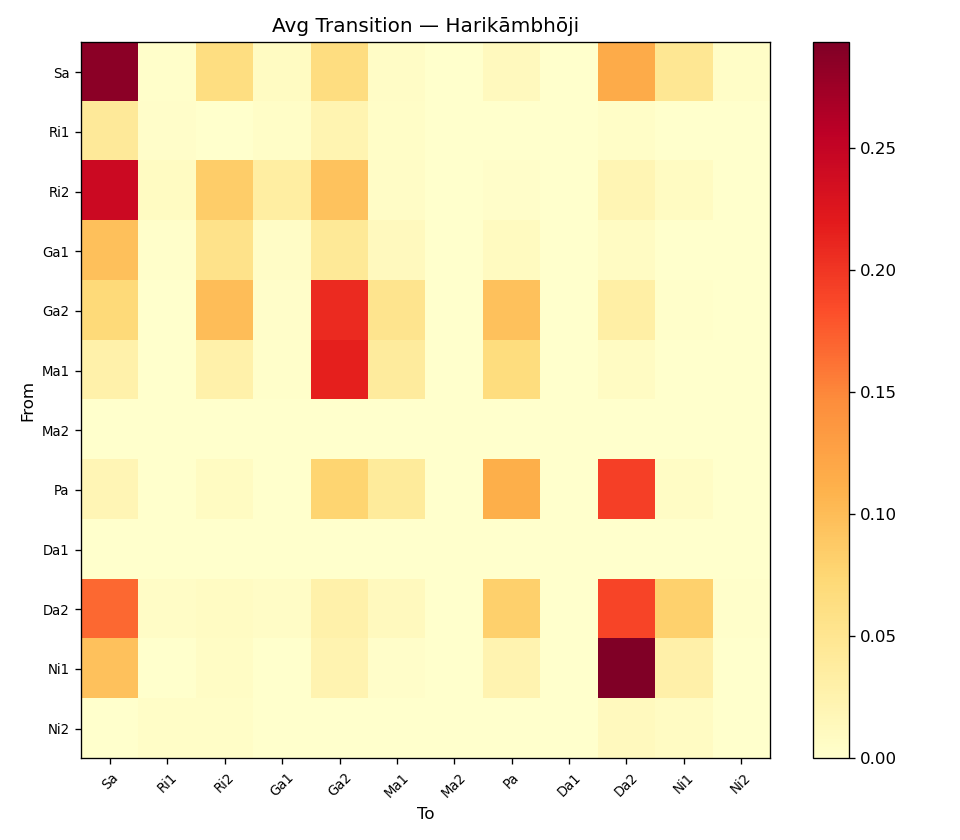
\includegraphics[width=\textwidth]{outputs/figures/features/transition_Harikambhoji.png}
\caption{Harik\=ambh\=oji (parent, 0\% F1)}
\end{subfigure}
\hfill
\begin{subfigure}[b]{0.48\textwidth}
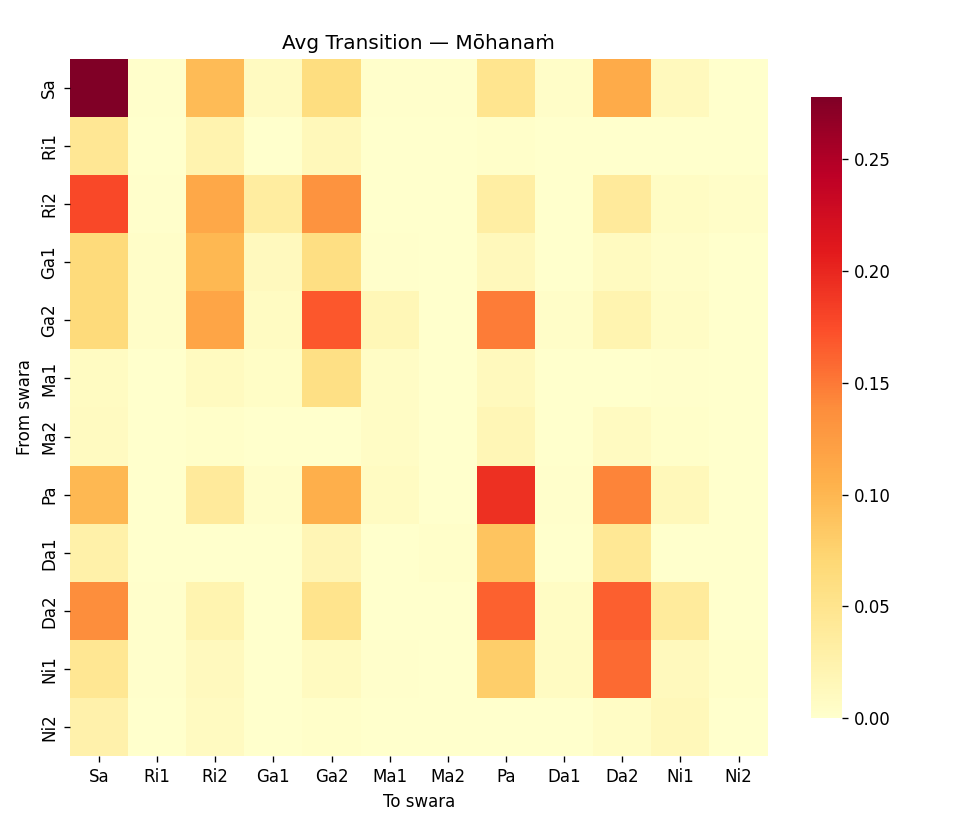
\includegraphics[width=\textwidth]{outputs/figures/features/transition_Mohanam.png}
\caption{M\=ohana\.{m} (pentatonic child)}
\end{subfigure}
\caption{Harik\=ambh\=oji vs M\=ohana\.{m} transitions. The parent's matrix is a dense superset; the child's is a sparse $5\times5$ subset. Kam\=as's transitions (above) are nearly identical to the parent's --- the root cause of within-family confusion.}
\label{fig:app-transition-2}
\end{figure}

\subsection{Directional Features (\=Arohana / Avarohana)}

\begin{figure}[H]
\centering
\begin{subfigure}[b]{0.48\textwidth}
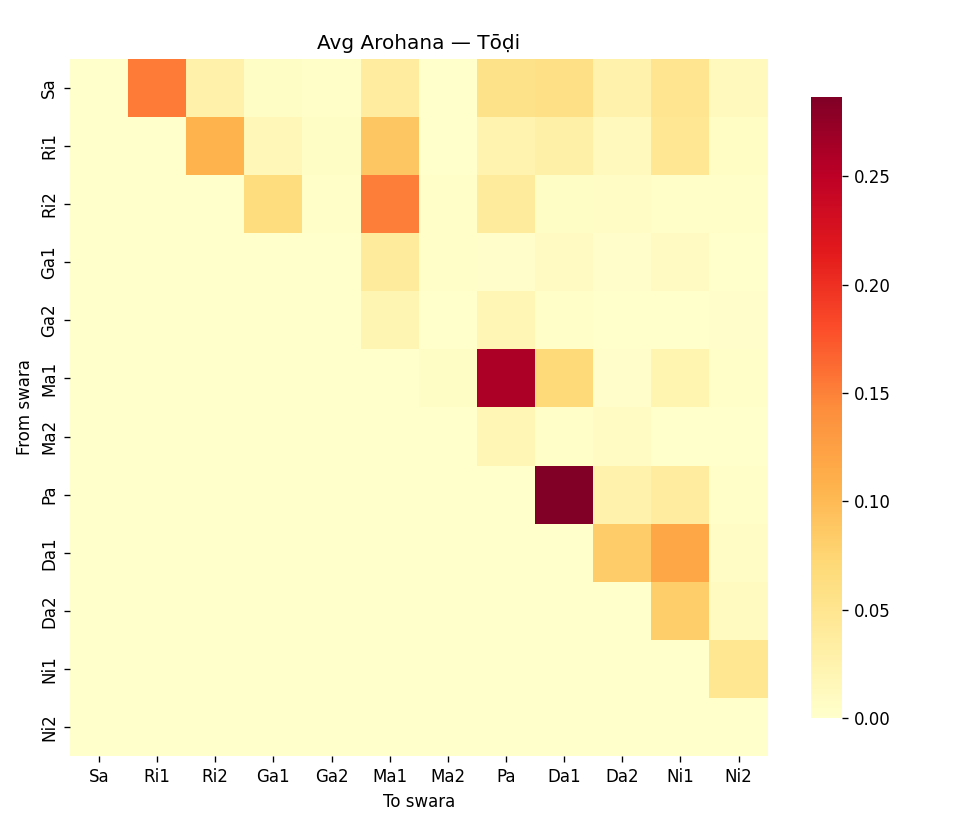
\includegraphics[width=\textwidth]{outputs/figures/features/arohana_Todi.png}
\caption{T\=o\d{d}i ascending (\=arohana)}
\end{subfigure}
\hfill
\begin{subfigure}[b]{0.48\textwidth}
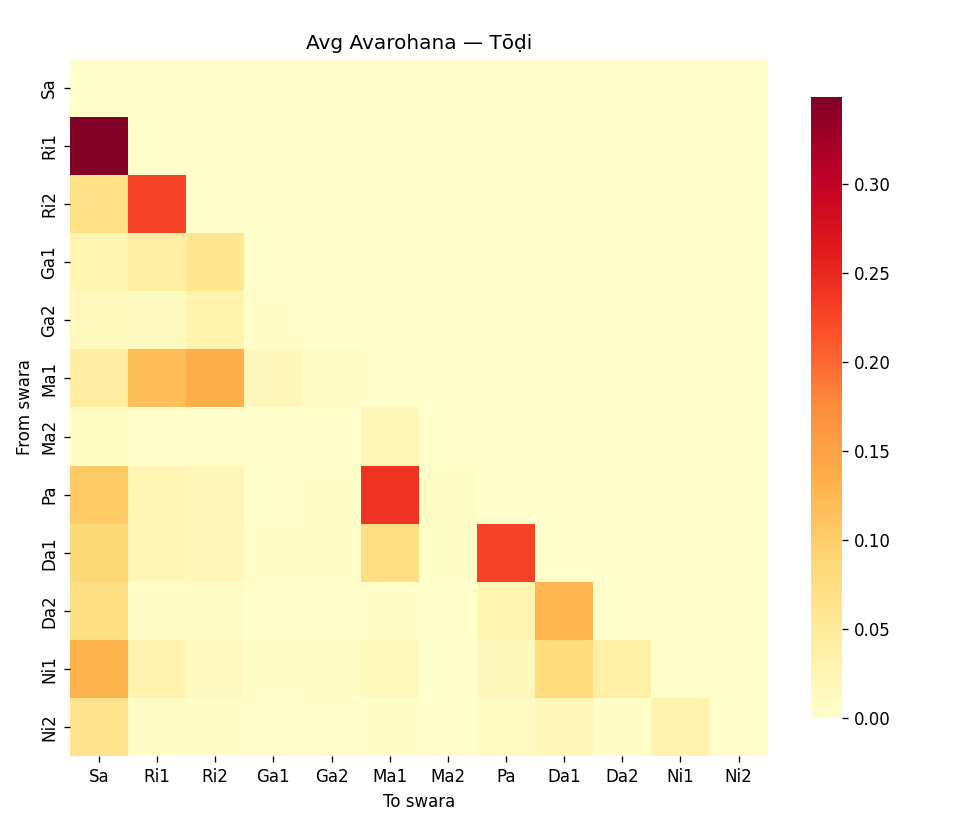
\includegraphics[width=\textwidth]{outputs/figures/features/avarohana_Todi.png}
\caption{T\=o\d{d}i descending (avarohana)}
\end{subfigure}
\caption{Directional PCD for T\=o\d{d}i. Tested under H6; directional encoding did not improve classification because gamakas blur the ascending/descending distinction in performed Carnatic music.}
\label{fig:app-directional}
\end{figure}

% ══════════════════════════════════════════════════════════
\section{Stage 6: Classification}
% ══════════════════════════════════════════════════════════

\subsection{Per-\textit{Raga} Classification Performance}
\label{sec:app-perraga}

\begin{figure}[H]
\centering
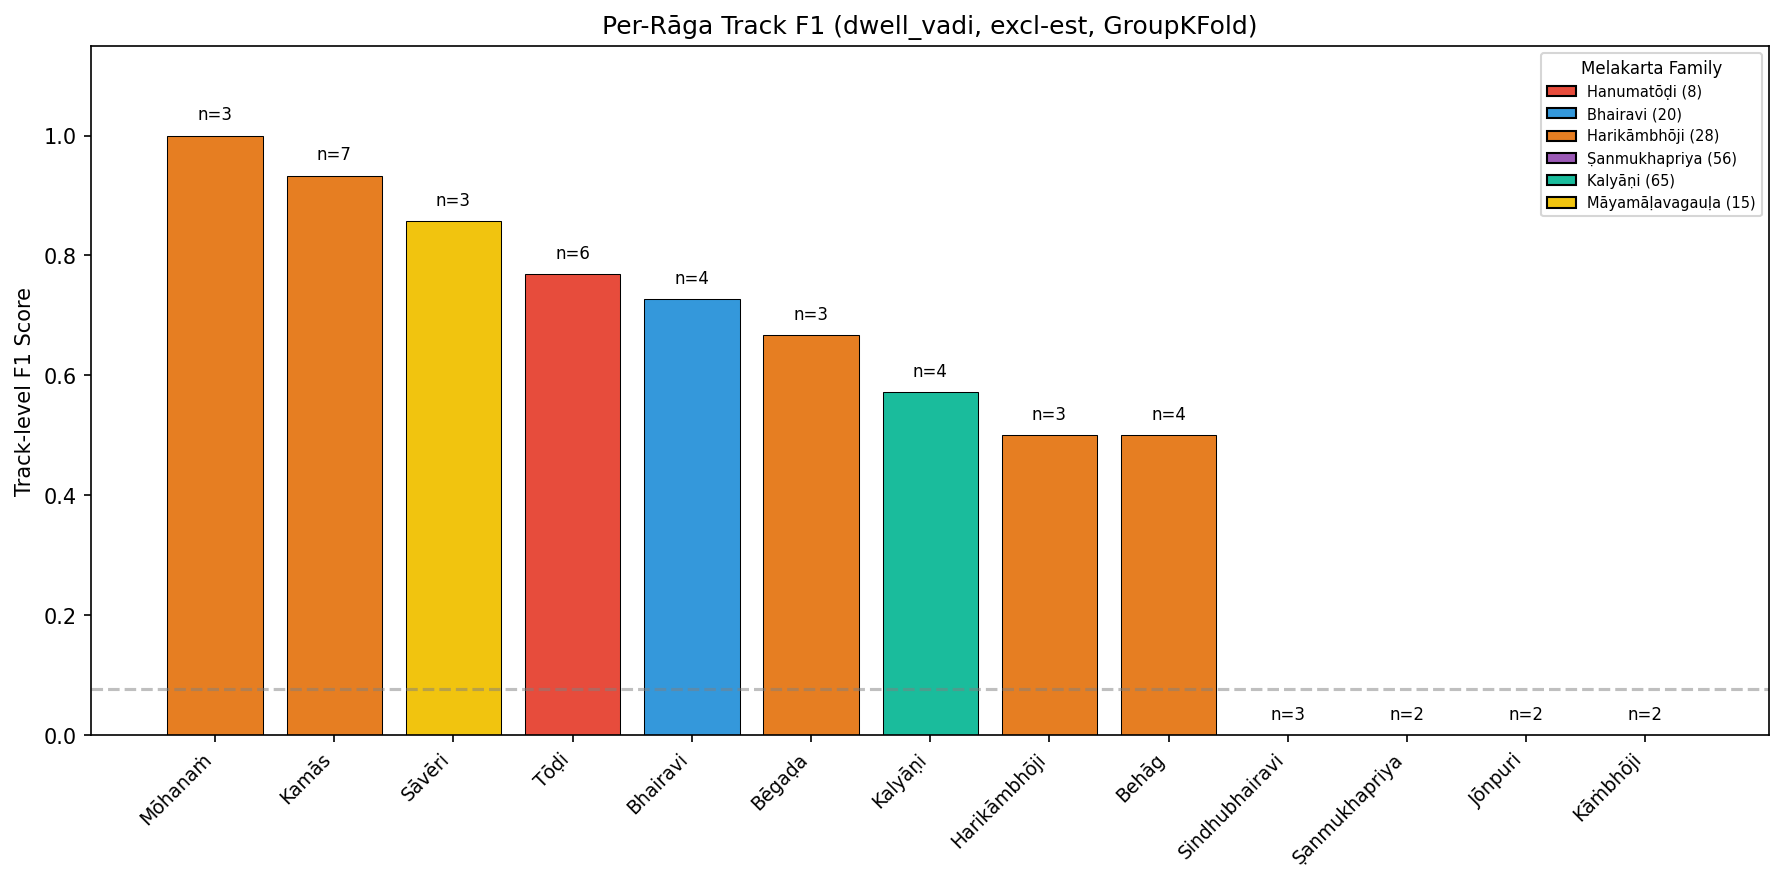
\includegraphics[width=0.85\textwidth]{outputs/figures/classification/excl-est/per_raga_f1_dwell_vadi.png}
\caption{Per-\textit{raga} track-level F1 scores for the best-performing model (dwell\_vadi, 16d) under the primary evaluation setting (excl-est, 13 \textit{ragas}, 46 tracks). Bars are coloured by melakarta family. \textit{Ragas} with distinctive intervallic signatures (T\=o\d{d}i, M\=ohana\.{m}) achieve high F1, while Harik\=ambh\=oji-family siblings (K\=a\d{m}bh\=oji, Sindhubhairavi) score near zero---consistent with within-family confusion predicted by H4. Track counts (n) indicate the small evaluation set per \textit{raga}.}
\label{fig:app-perraga-f1}
\end{figure}

\subsection{Primary Feature Sets}
\label{sec:app-confusion}

\begin{figure}[H]
\centering
\begin{subfigure}[b]{0.48\textwidth}
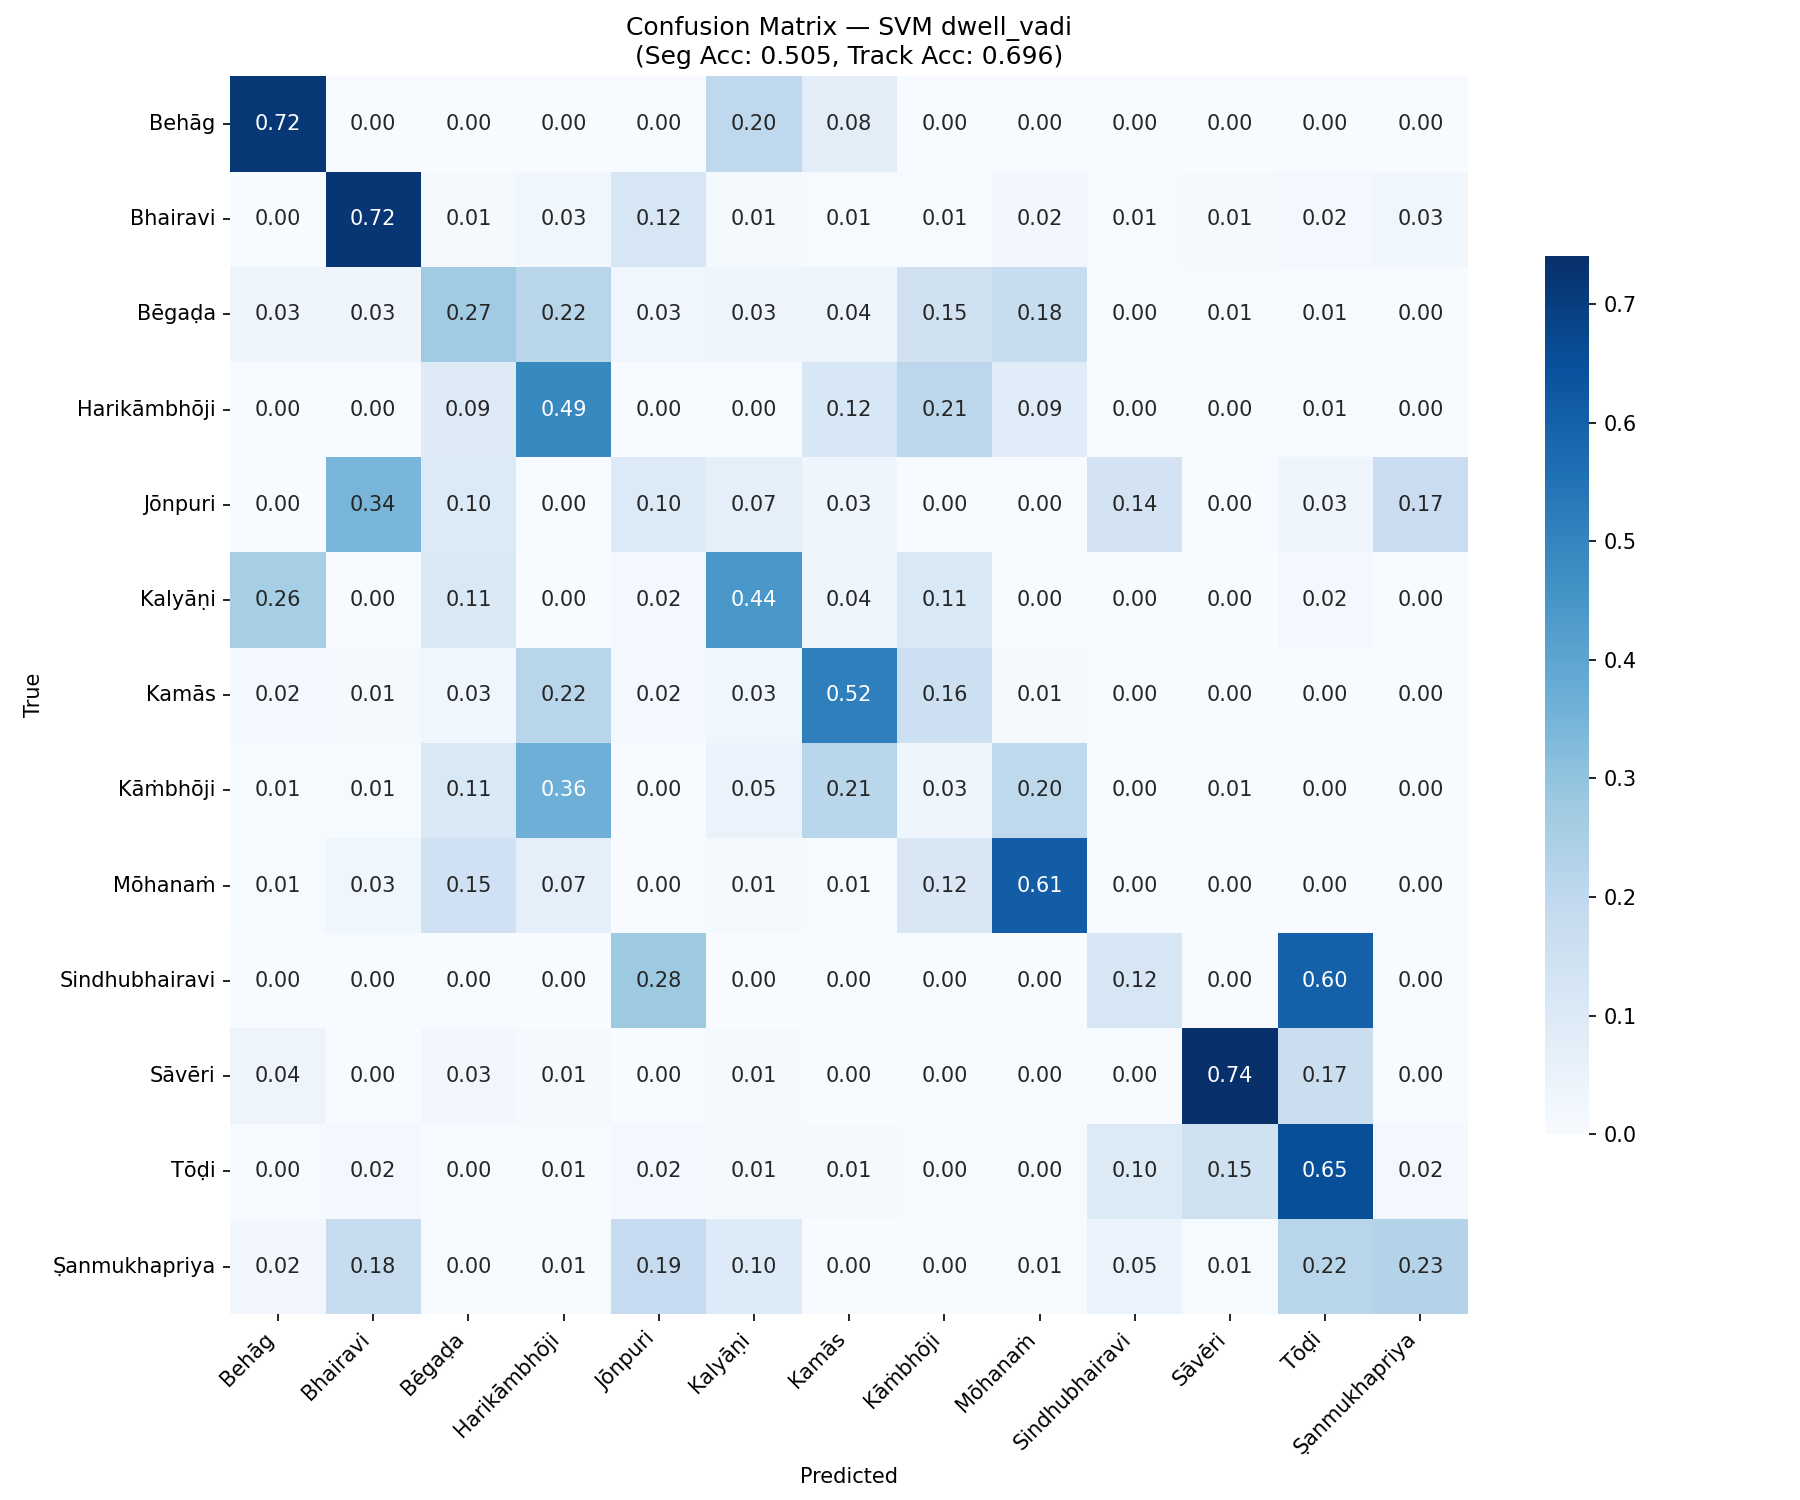
\includegraphics[width=\textwidth]{outputs/figures/classification/excl-est/cm_SVM_dwell_vadi.png}
\caption{Dwell + V\=adi (16d) --- 69.6\% track acc, 67.8\% F1w}
\end{subfigure}
\hfill
\begin{subfigure}[b]{0.48\textwidth}
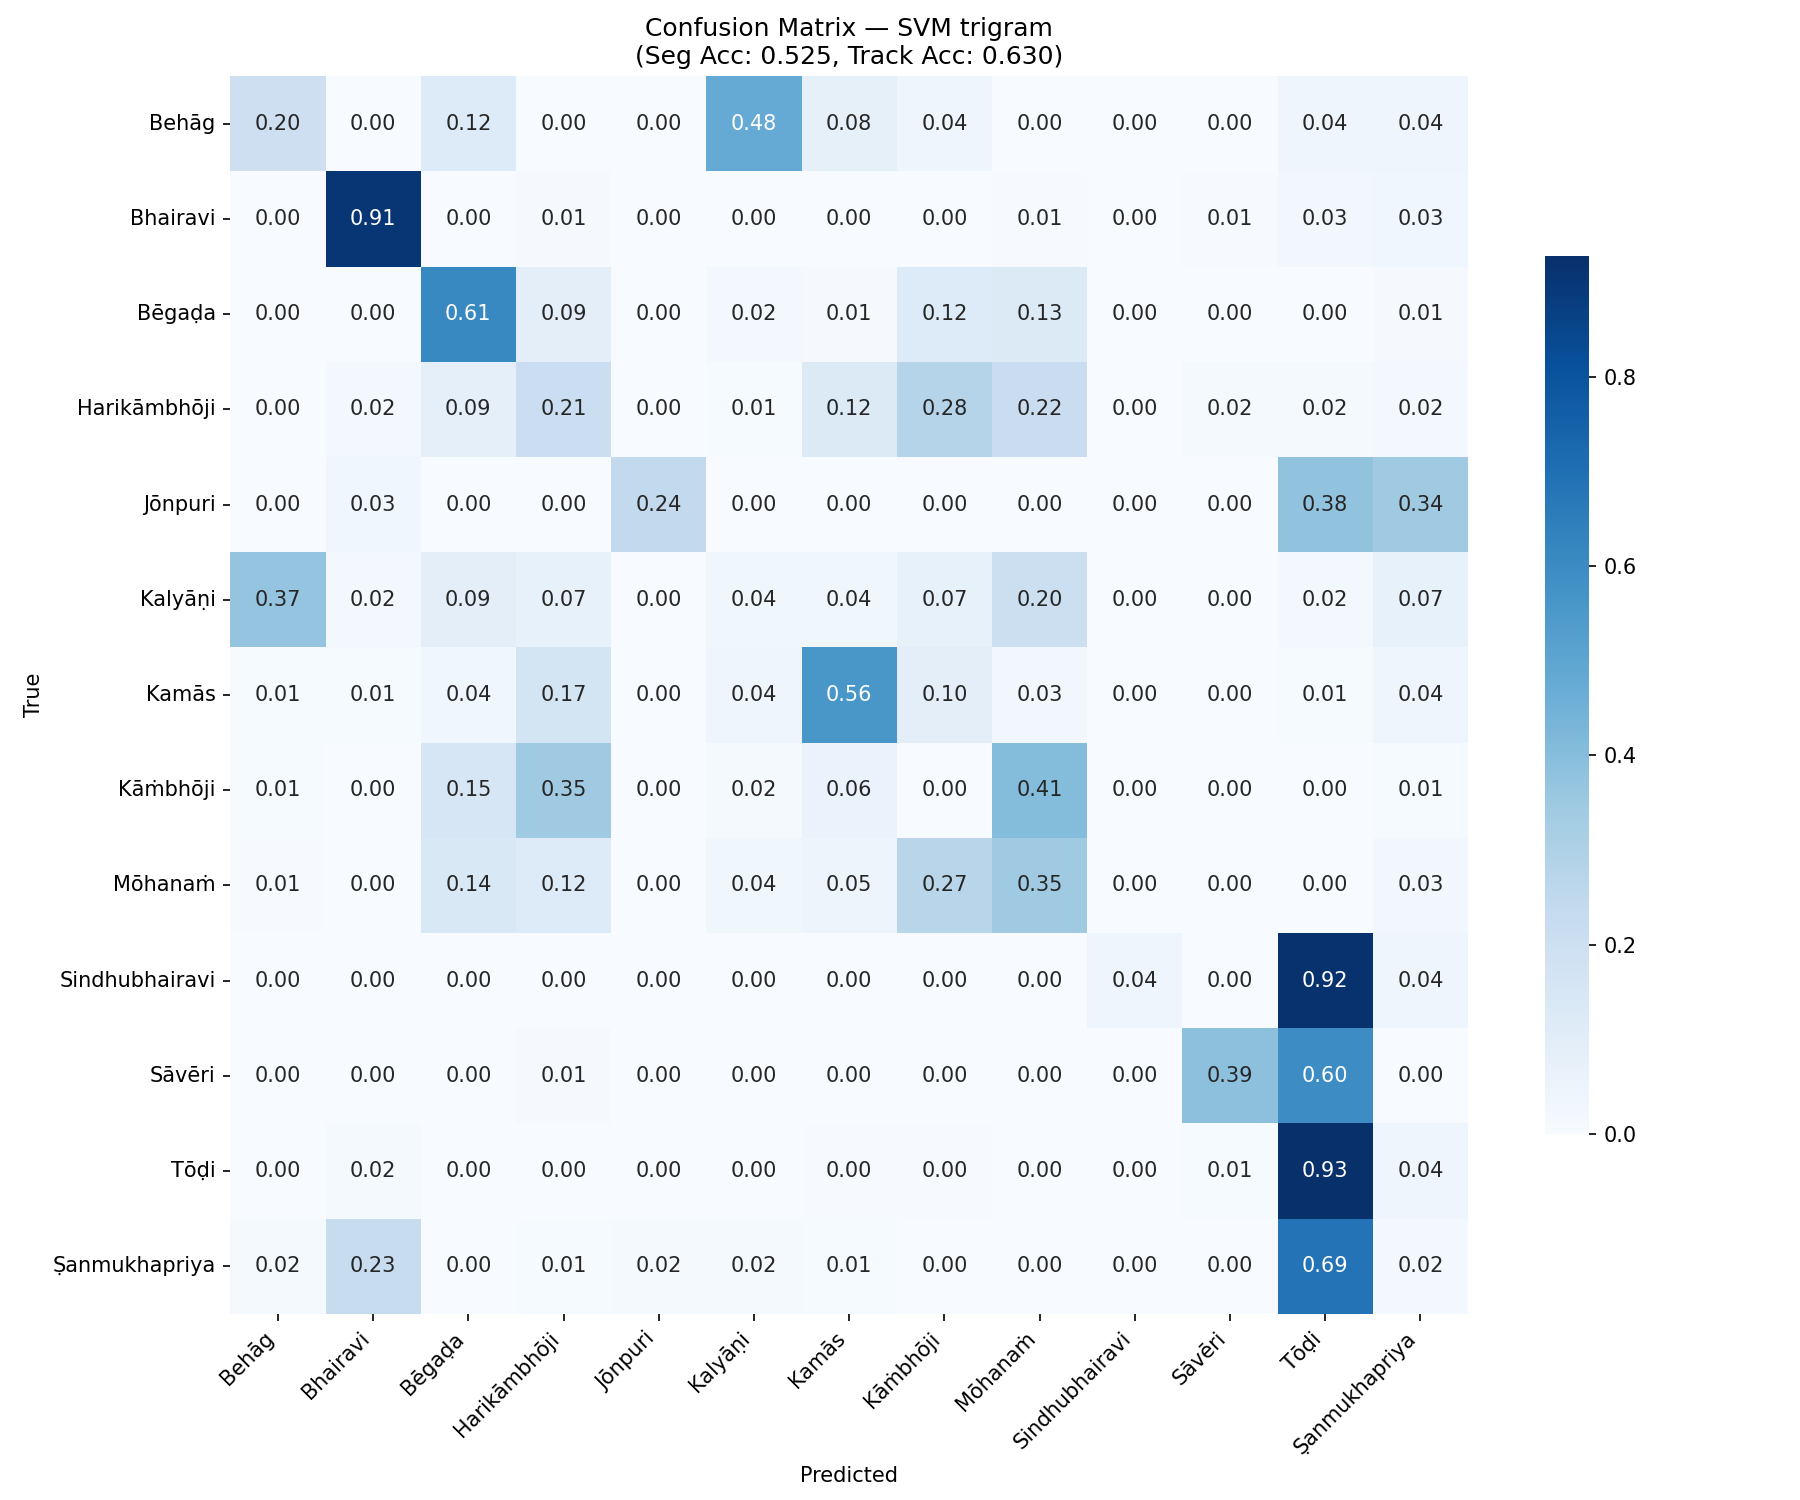
\includegraphics[width=\textwidth]{outputs/figures/classification/excl-est/cm_SVM_trigram.png}
\caption{Trigram (200d) --- 63.0\% track acc, 59.1\% F1w}
\end{subfigure}
\caption{Confusion matrices for the two best-performing single-feature models. Dwell + v\=adi achieves the highest track-level F1w despite using only 16 dimensions.}
\label{fig:app-cm-best}
\end{figure}

\begin{figure}[H]
\centering
\begin{subfigure}[b]{0.48\textwidth}
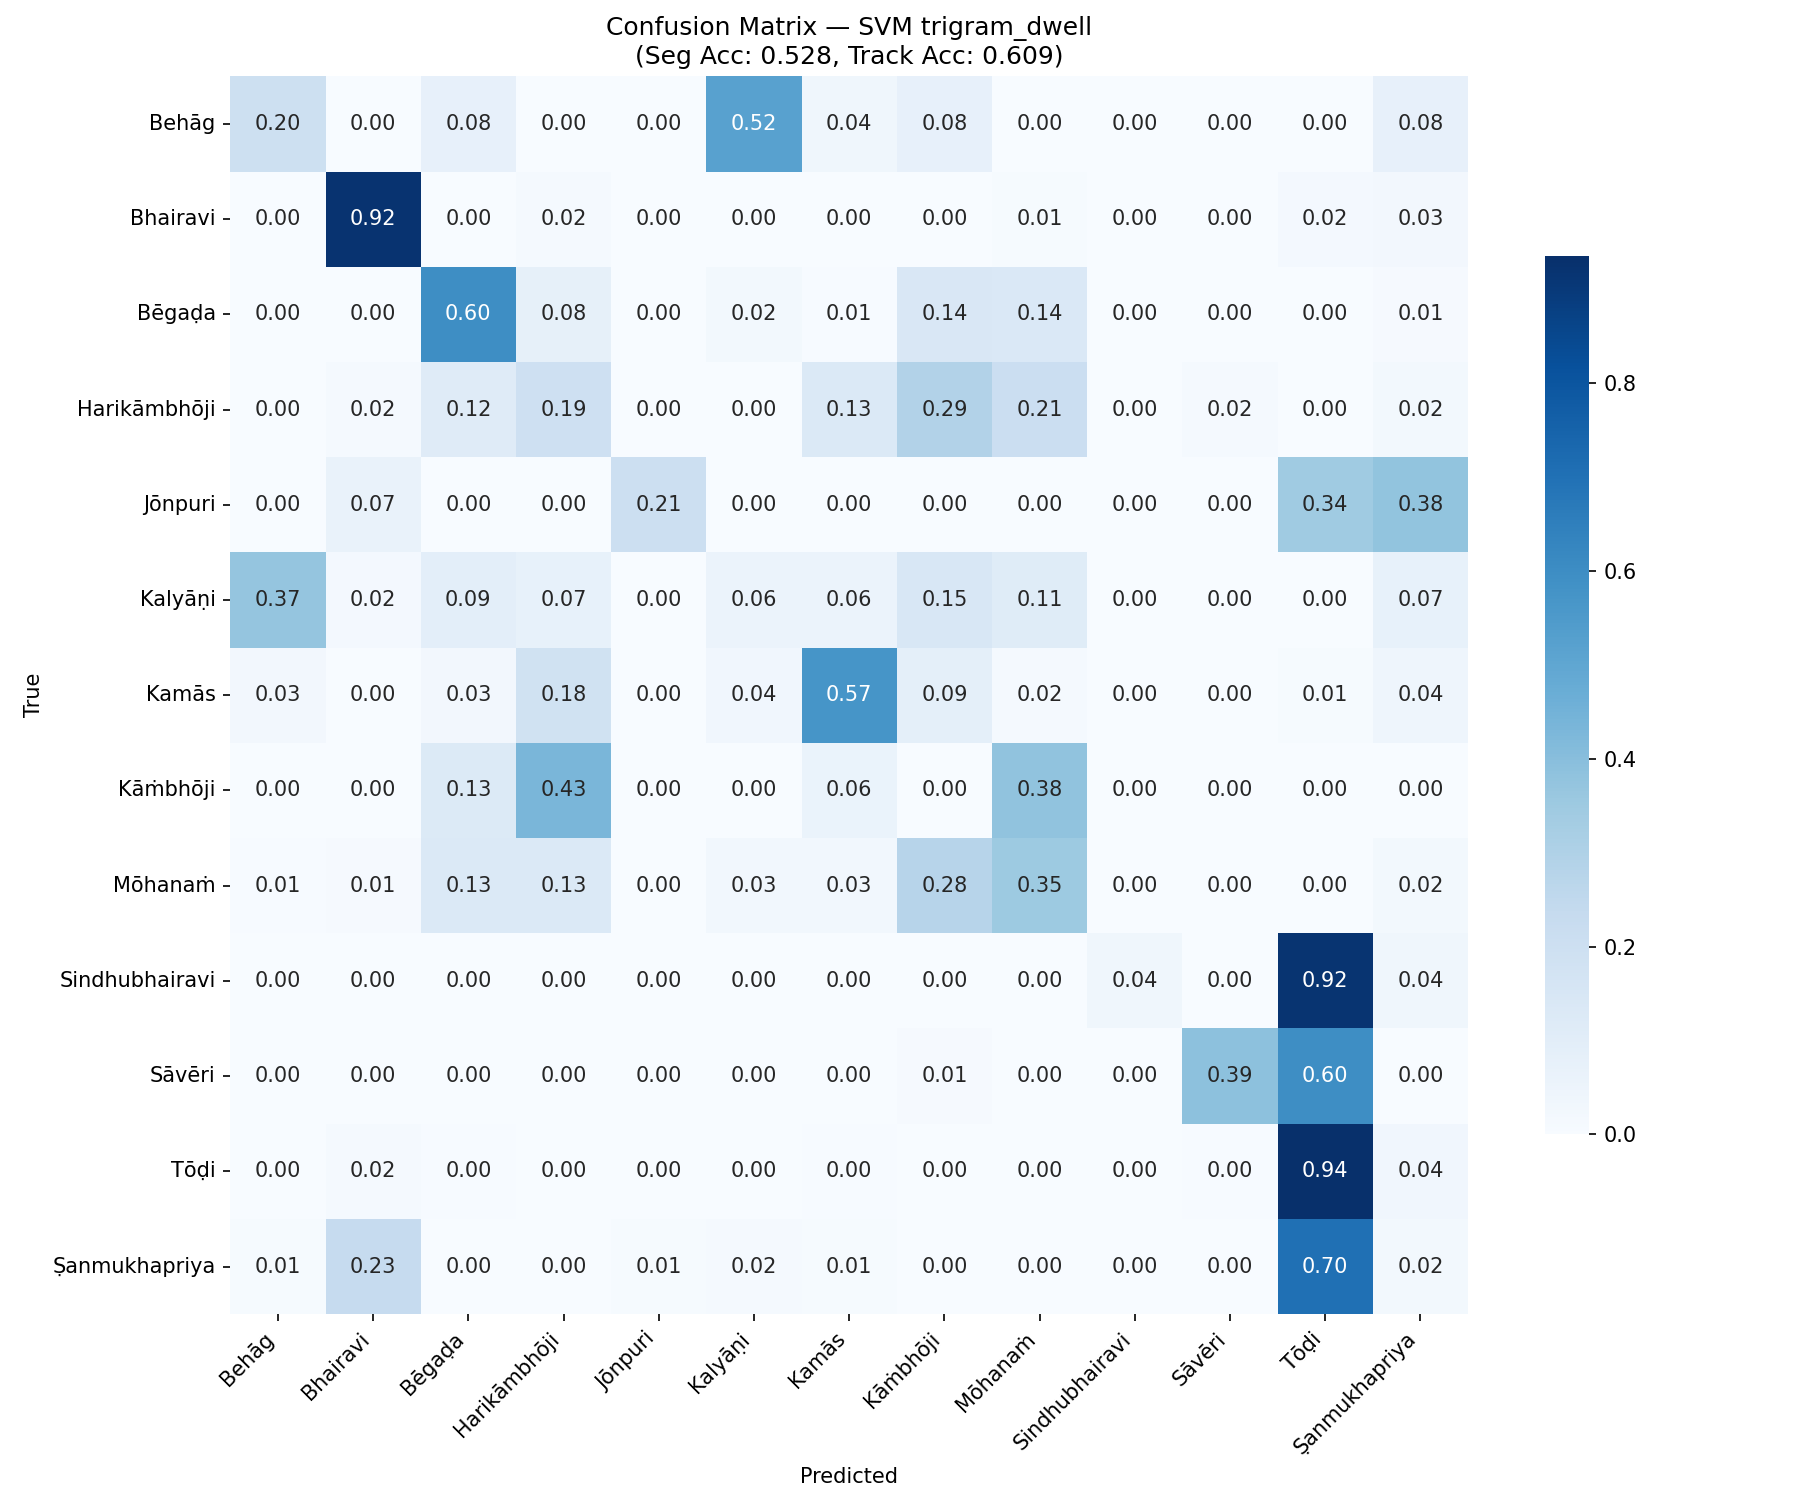
\includegraphics[width=\textwidth]{outputs/figures/classification/excl-est/cm_SVM_trigram_dwell.png}
\caption{Trigram + Dwell (216d) --- 60.9\% track acc, 57.2\% F1w}
\end{subfigure}
\hfill
\begin{subfigure}[b]{0.48\textwidth}
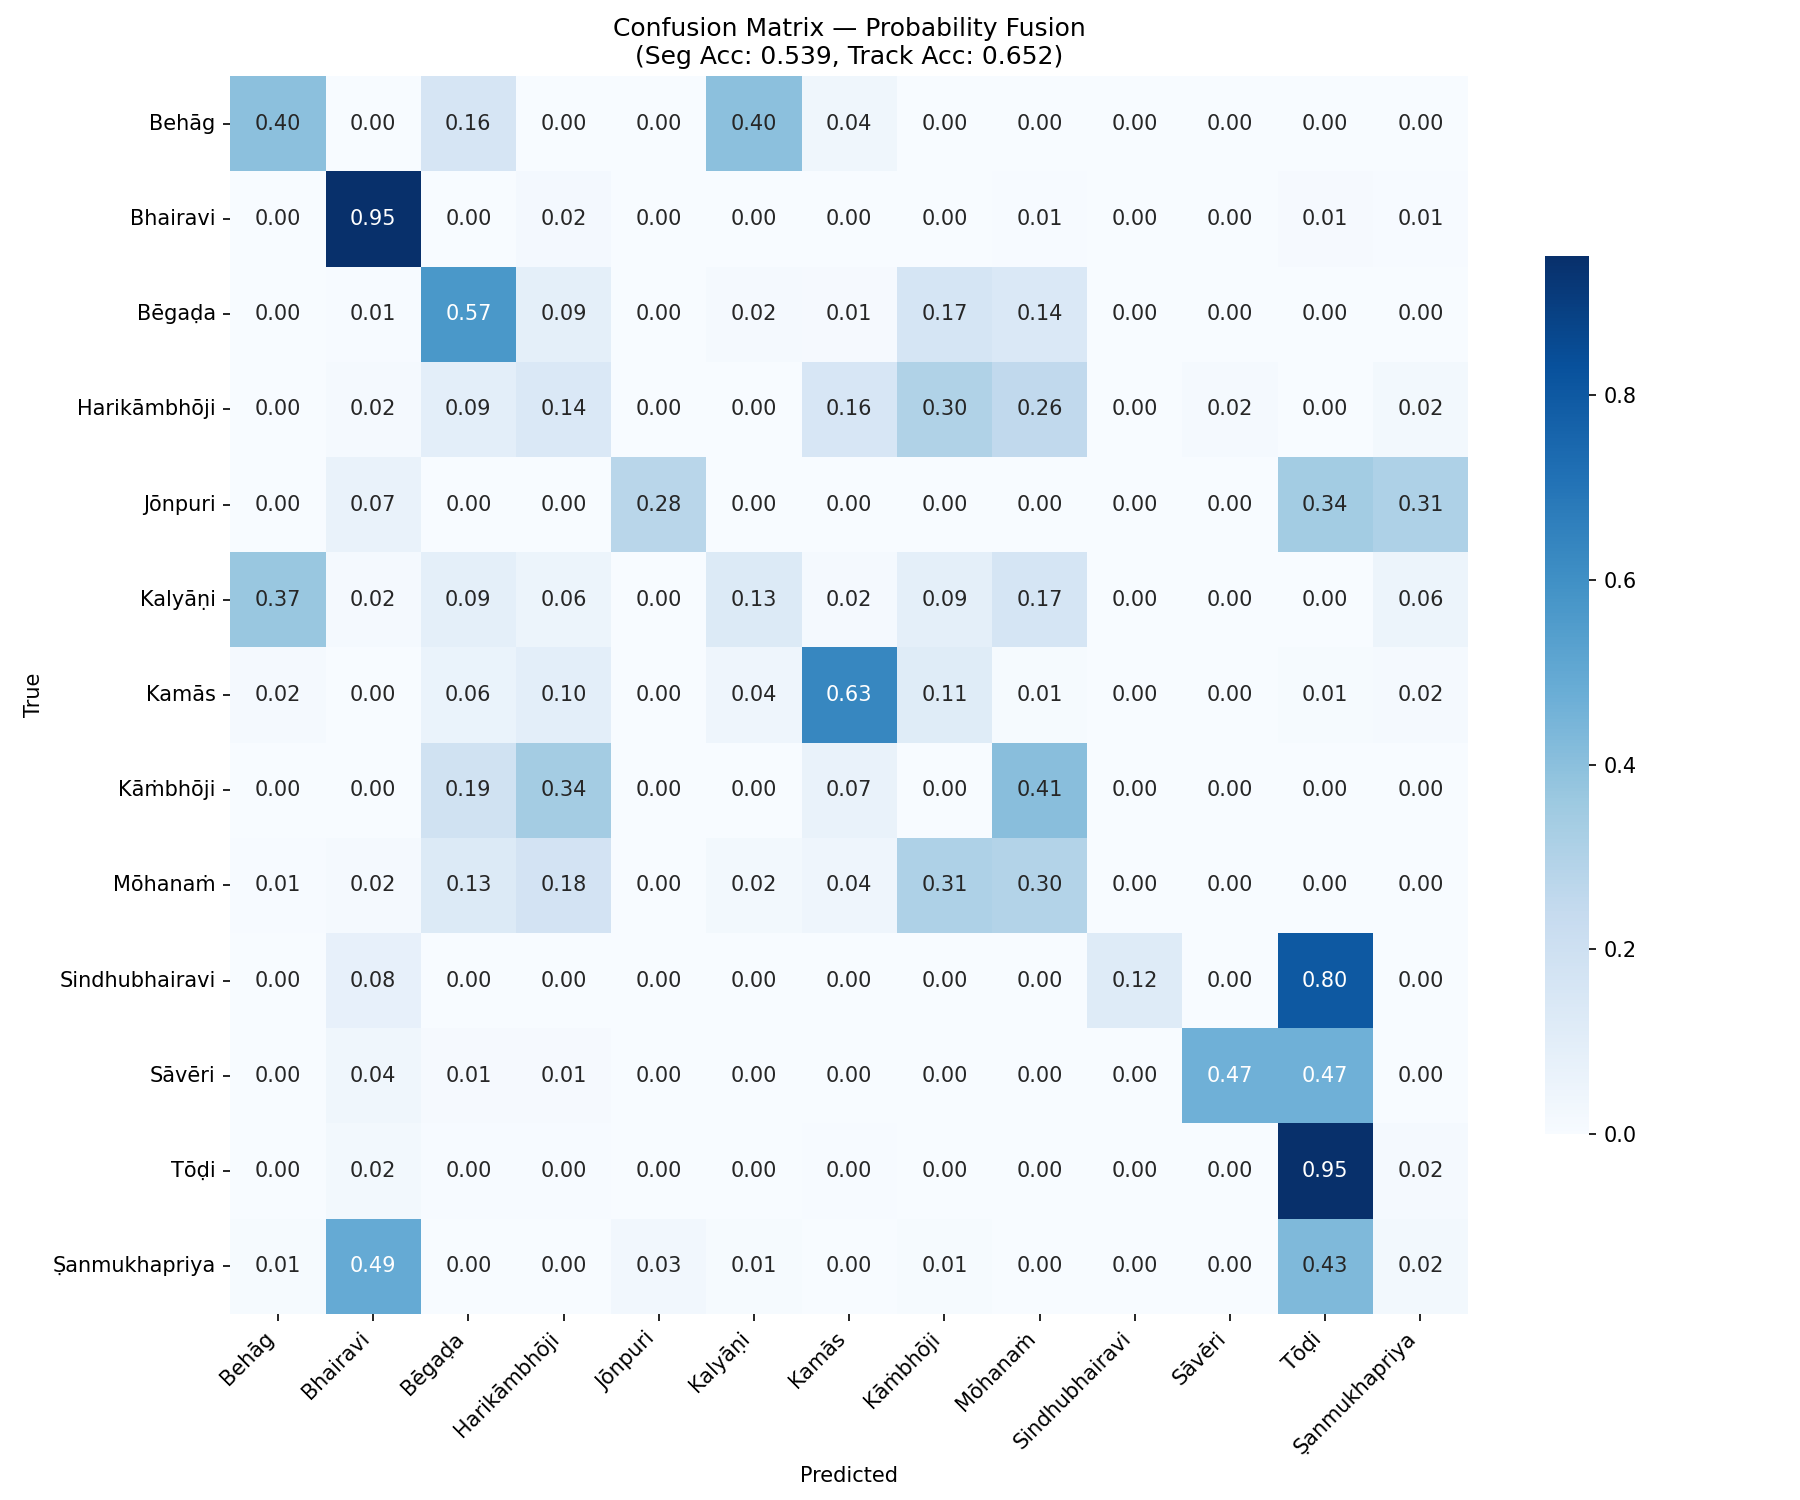
\includegraphics[width=\textwidth]{outputs/figures/classification/excl-est/cm_fusion_pitch.png}
\caption{Probability fusion --- 65.2\% track acc, 64.0\% F1w}
\end{subfigure}
\caption{Combined feature models. Fusion improves over individual models but does not exceed dwell + v\=adi in track-level F1w, supporting cognitive parsimony (H3).}
\label{fig:app-cm-combined}
\end{figure}

\subsection{Additional Feature Variants}

\begin{figure}[H]
\centering
\begin{subfigure}[b]{0.48\textwidth}
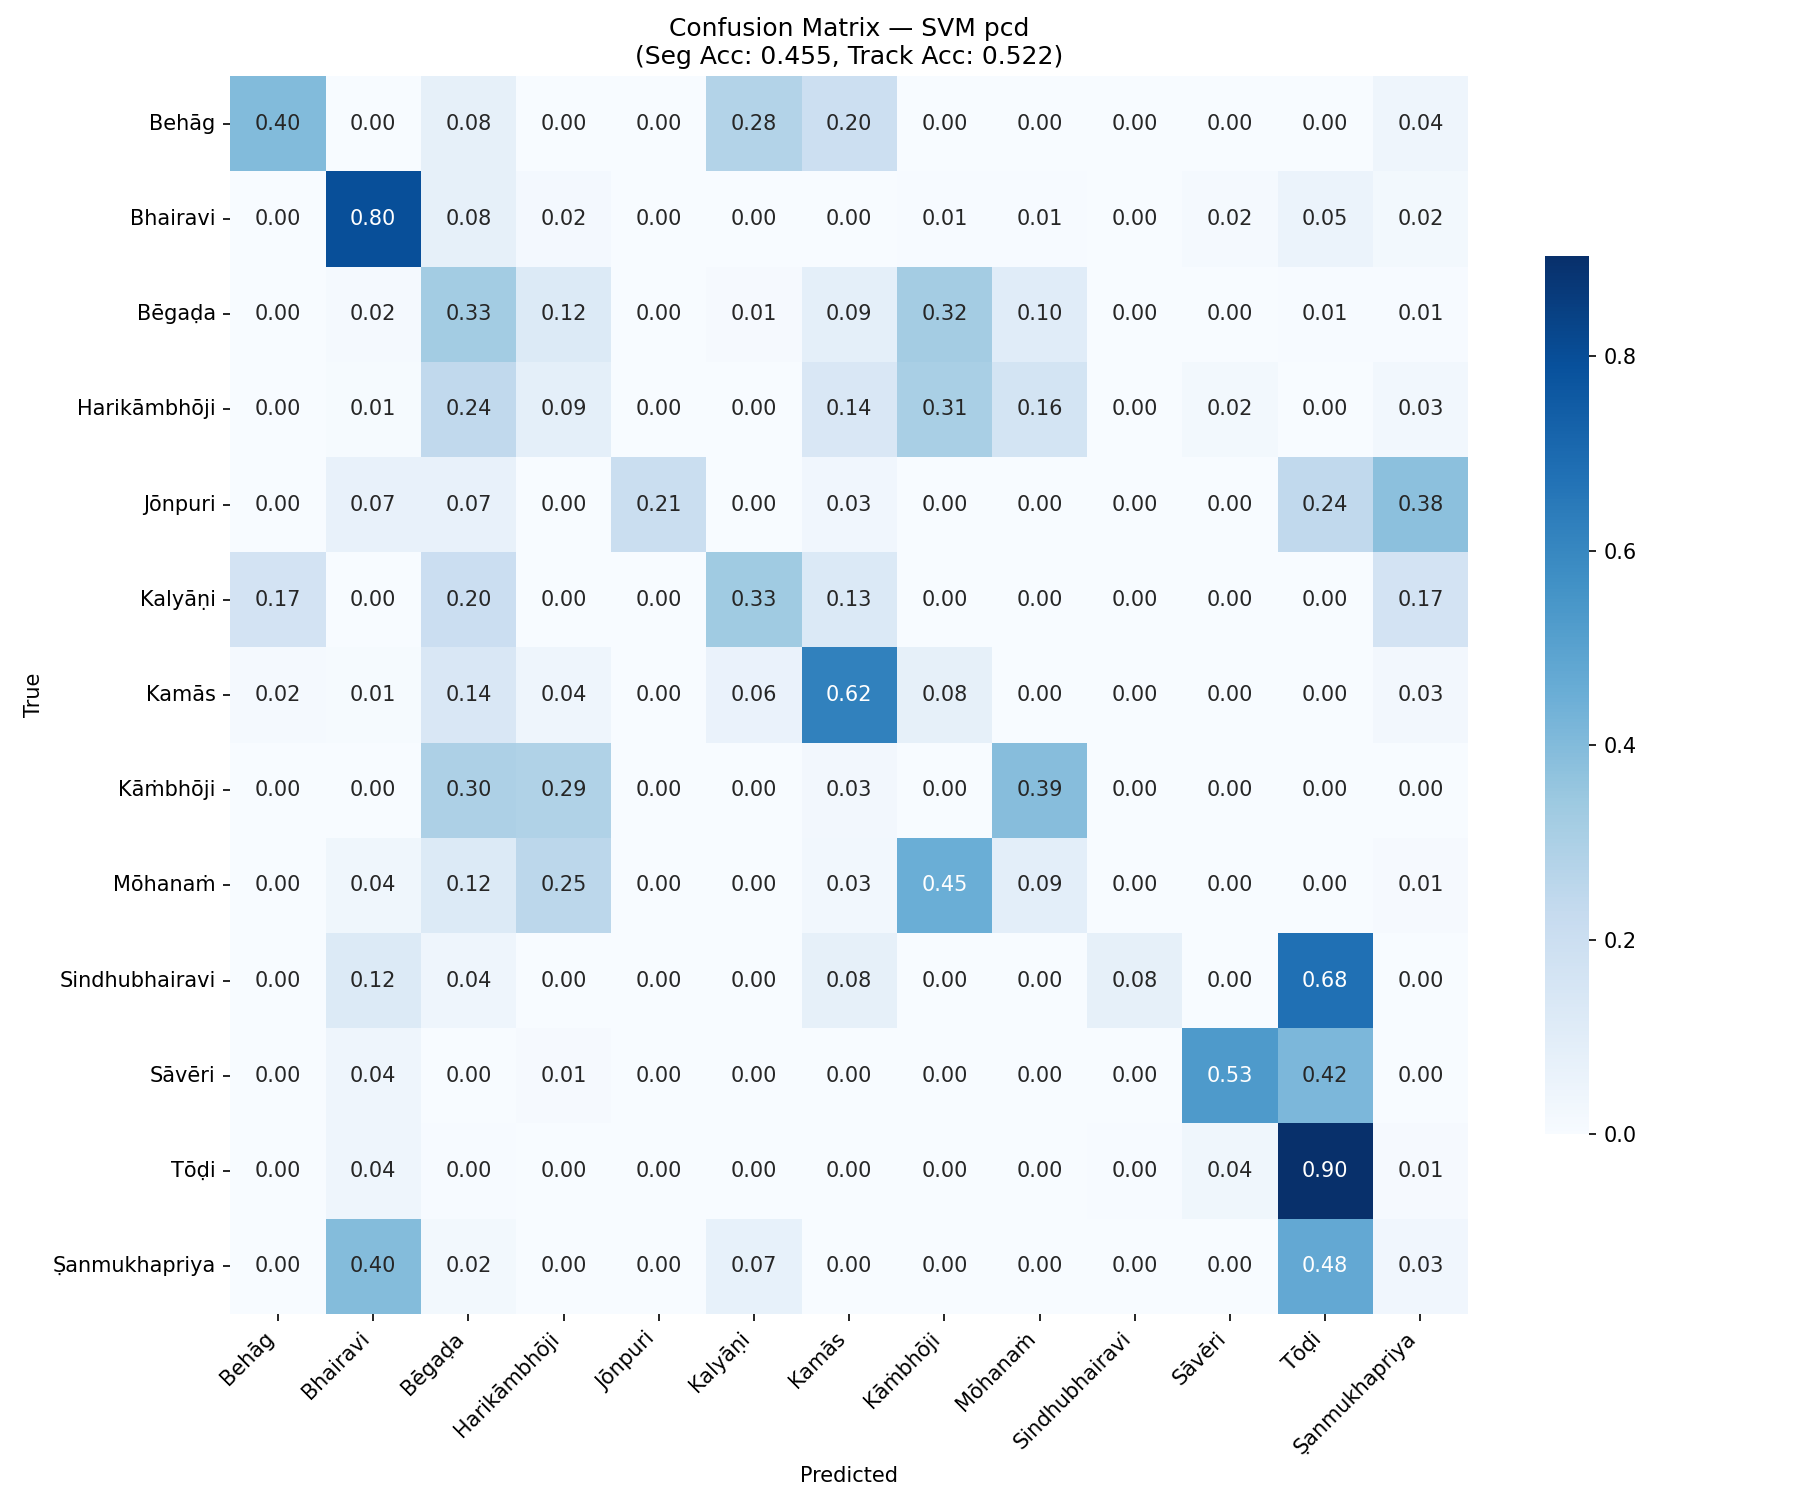
\includegraphics[width=\textwidth]{outputs/figures/classification/excl-est/cm_SVM_pcd.png}
\caption{PCD (120d) --- 52.2\% track acc, 49.6\% F1w}
\end{subfigure}
\hfill
\begin{subfigure}[b]{0.48\textwidth}
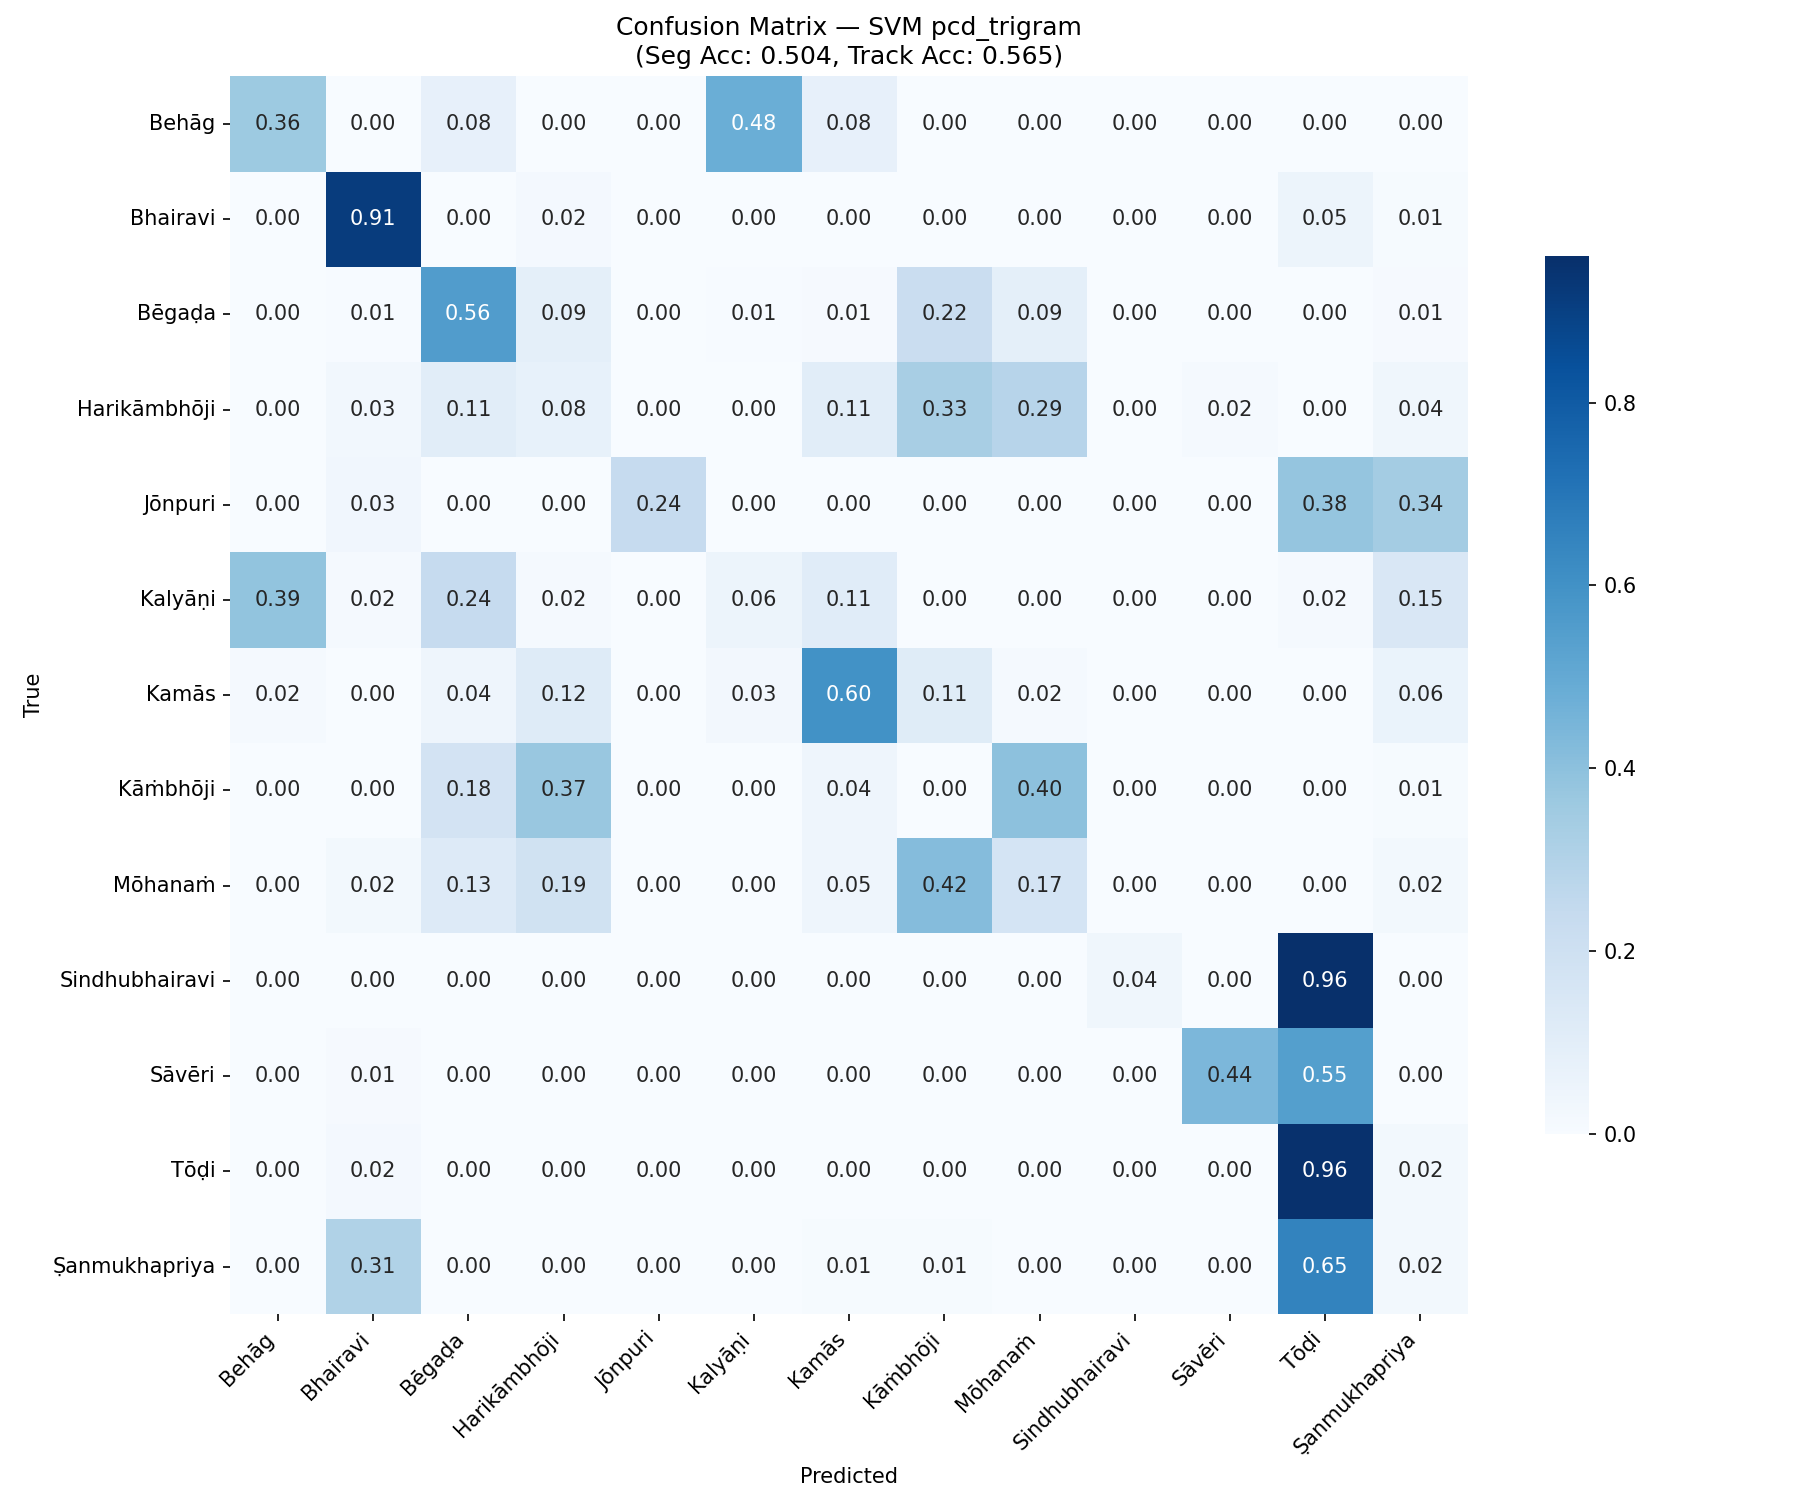
\includegraphics[width=\textwidth]{outputs/figures/classification/excl-est/cm_SVM_pcd_trigram.png}
\caption{PCD + Trigram (320d) --- 56.5\% track acc, 51.9\% F1w}
\end{subfigure}
\caption{PCD-based confusion matrices. Adding PCD to trigrams does not improve over trigrams alone (H3: cognitive parsimony).}
\label{fig:app-cm-pcd}
\end{figure}

\begin{figure}[H]
\centering
\begin{subfigure}[b]{0.48\textwidth}
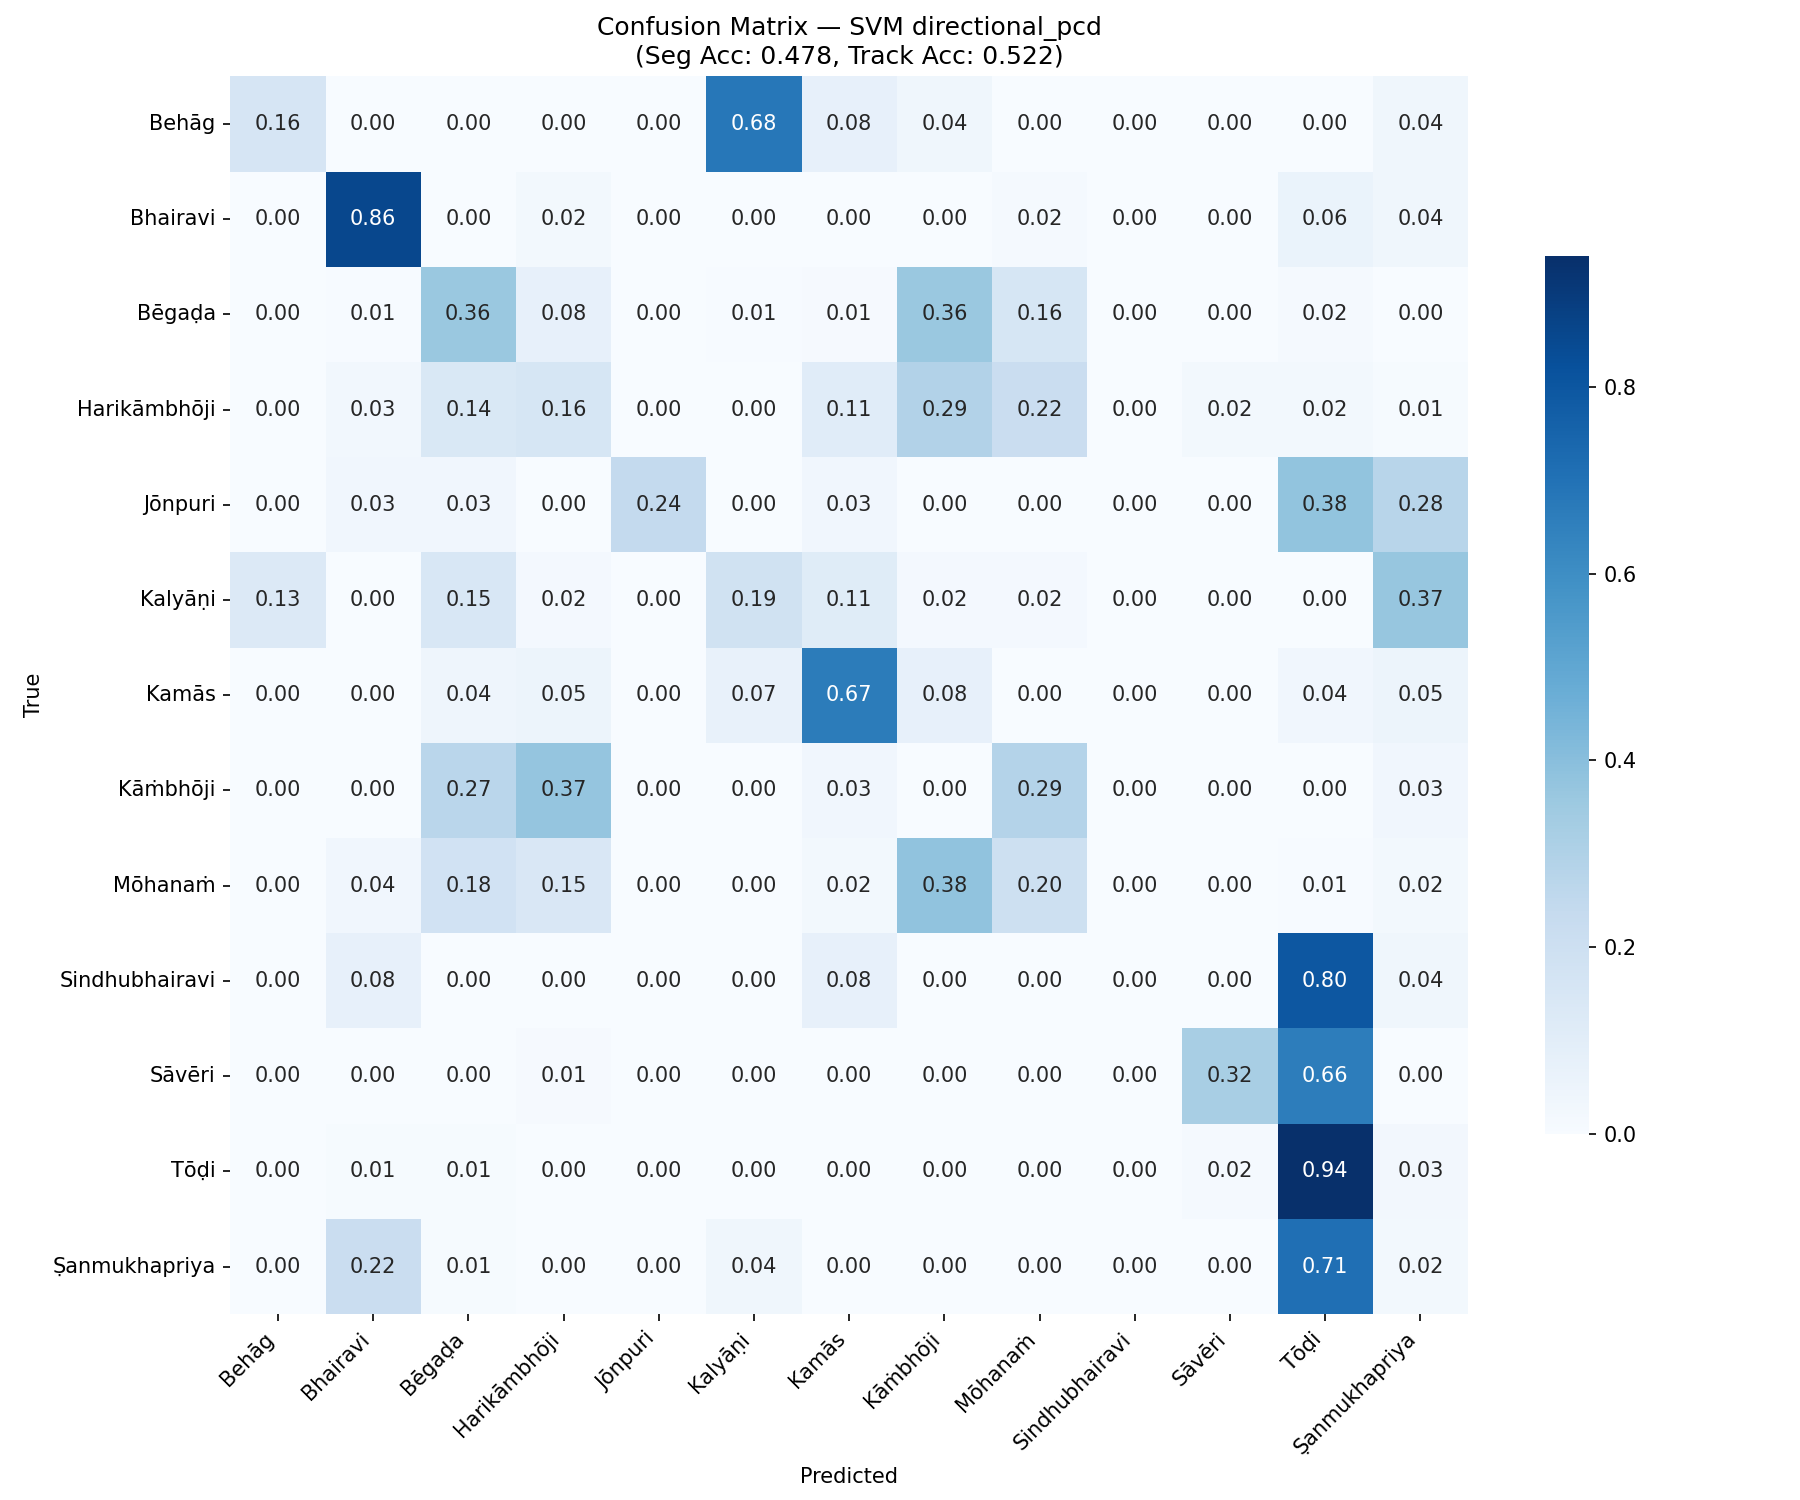
\includegraphics[width=\textwidth]{outputs/figures/classification/excl-est/cm_SVM_directional_pcd.png}
\caption{Directional PCD (408d) --- 52.2\% track acc, 49.1\% F1w}
\end{subfigure}
\hfill
\begin{subfigure}[b]{0.48\textwidth}
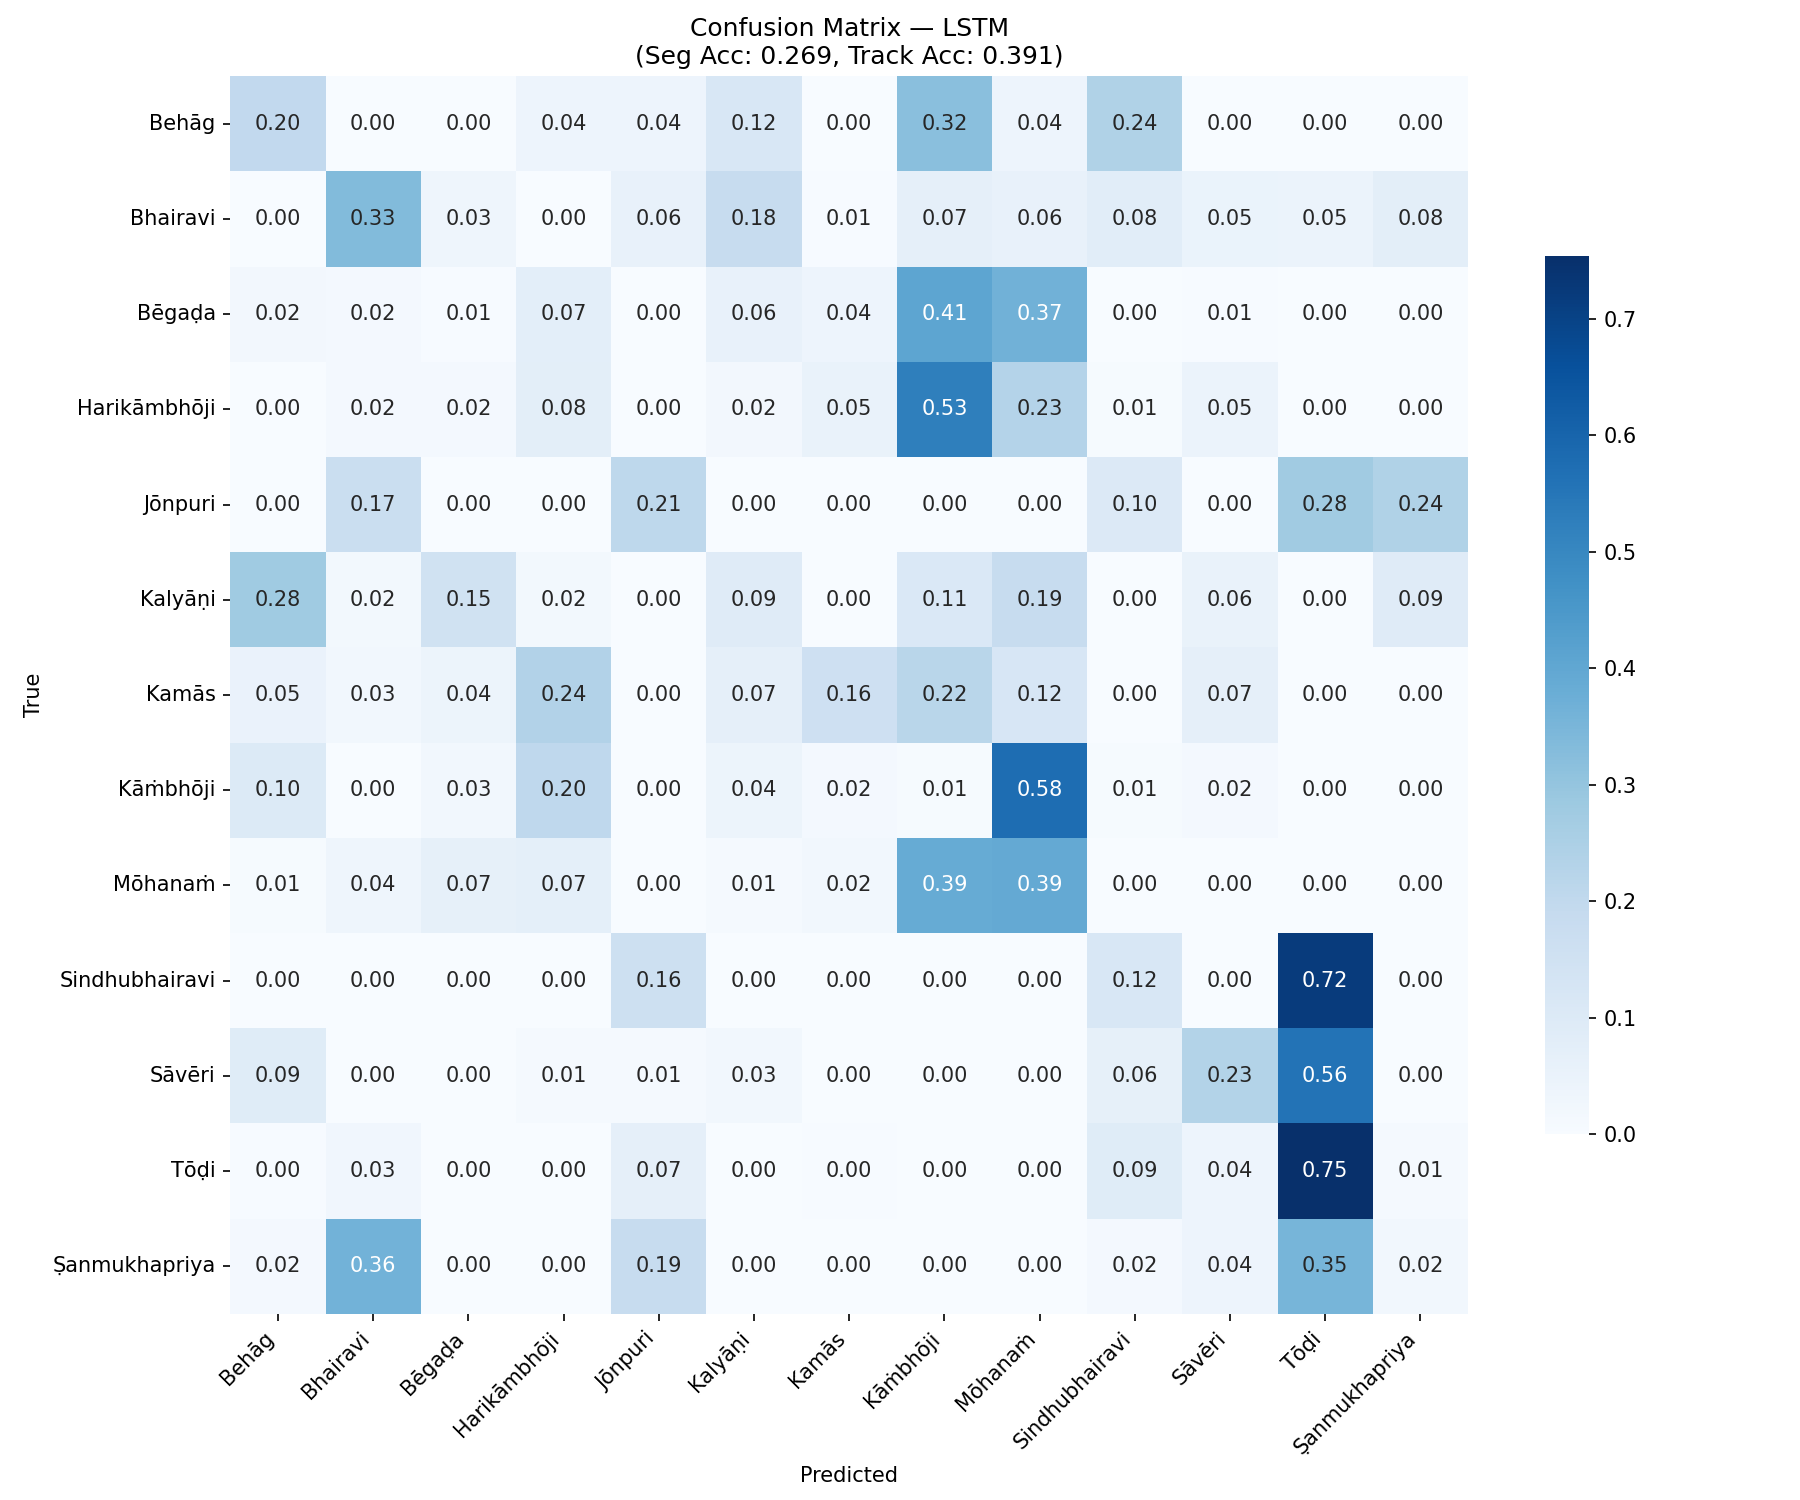
\includegraphics[width=\textwidth]{outputs/figures/classification/excl-est/cm_LSTM_swara_seq.png}
\caption{BiLSTM --- 39.1\% track acc, 36.4\% F1w}
\end{subfigure}
\caption{Directional features (H6, does not improve) and deep learning baseline. The BiLSTM suffers from data starvation (1,648 segments after filtering).}
\label{fig:app-cm-directional-lstm}
\end{figure}

\subsection{H4: Melakarta Family Confusion Analysis}
\label{sec:app-h4}

\begin{figure}[H]
\centering
\begin{subfigure}[b]{0.48\textwidth}
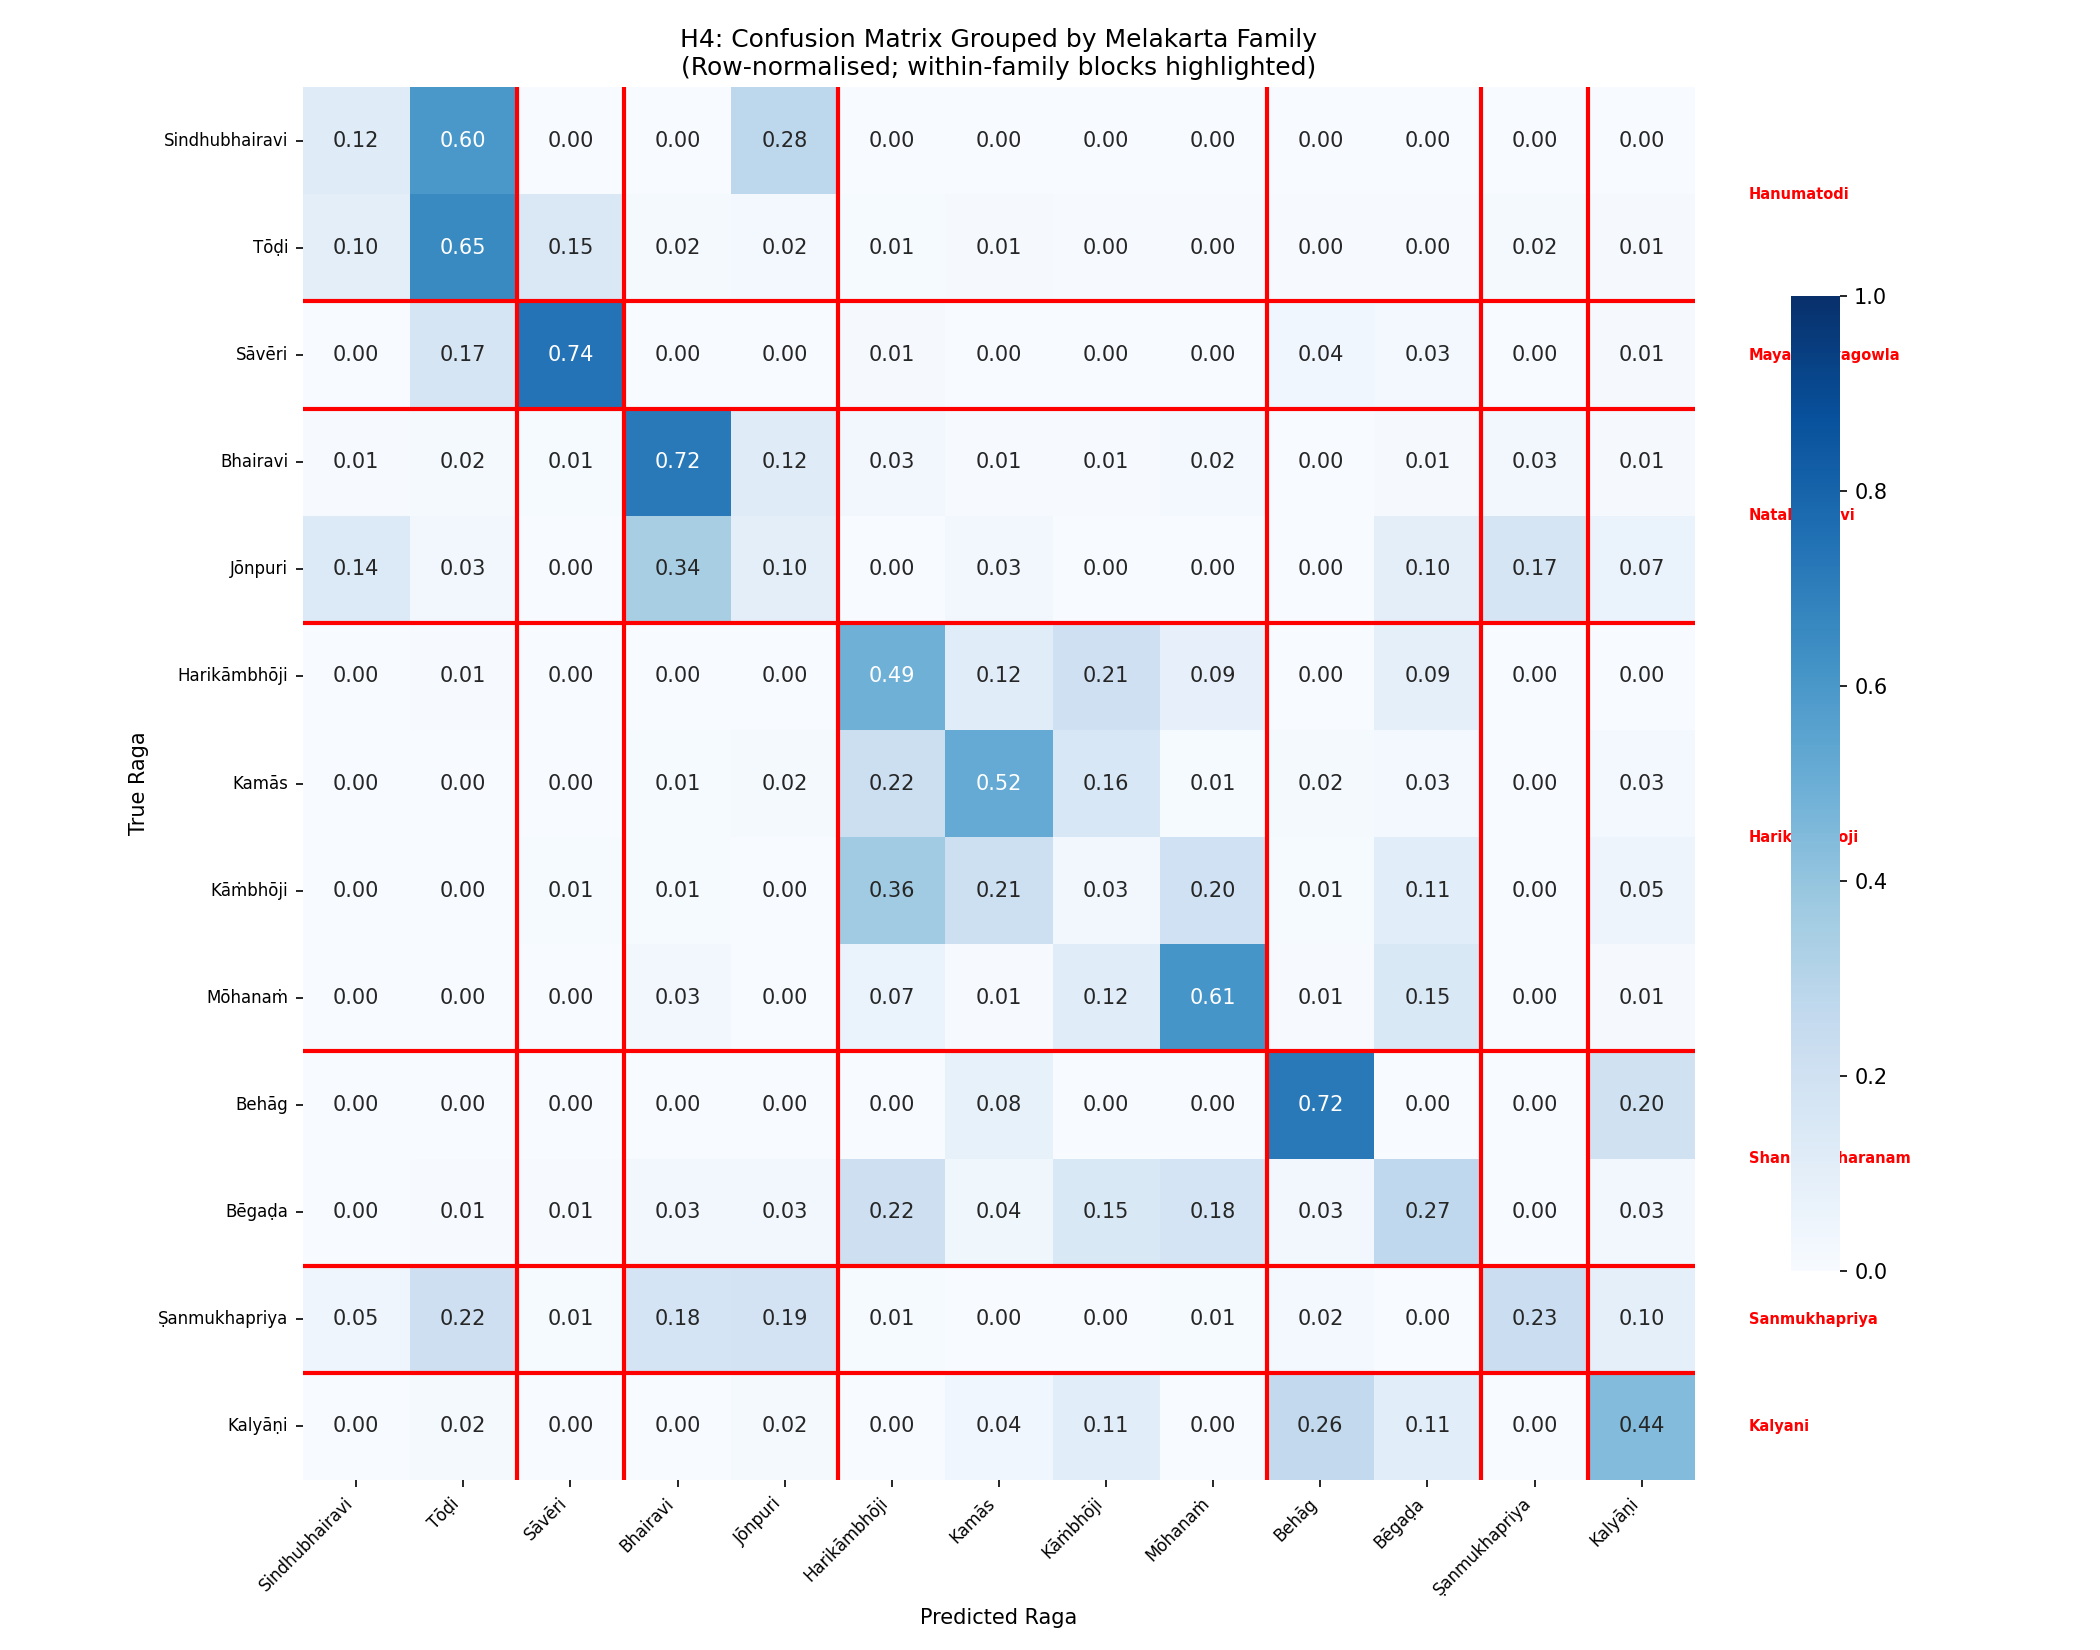
\includegraphics[width=\textwidth]{outputs/figures/h4_melakarta/confusion_matrix_by_family.png}
\caption{Confusion matrix annotated by melakarta family}
\end{subfigure}
\hfill
\begin{subfigure}[b]{0.48\textwidth}
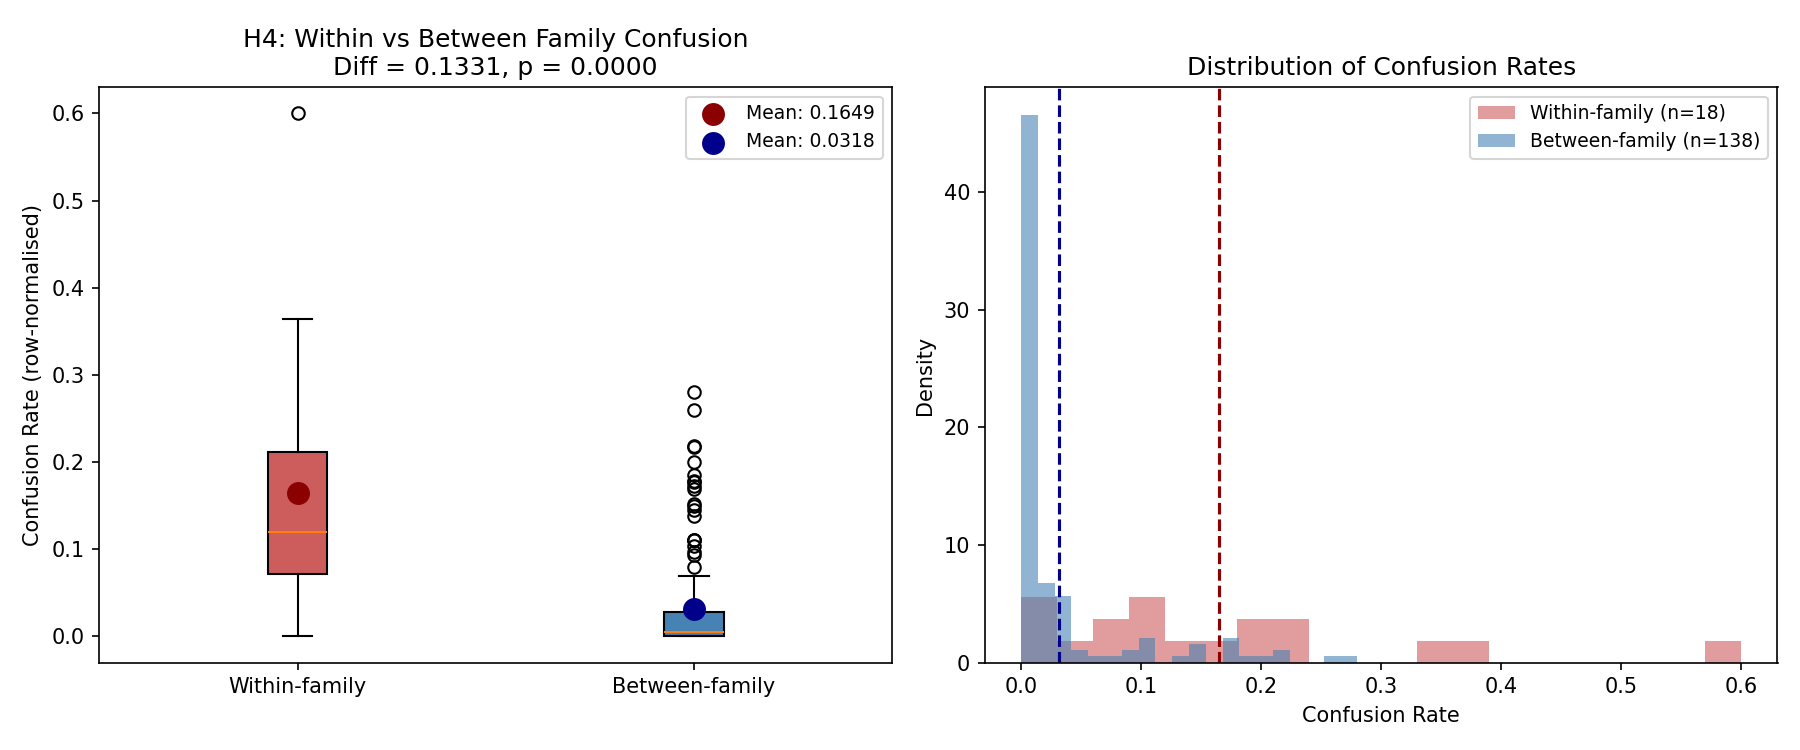
\includegraphics[width=\textwidth]{outputs/figures/h4_melakarta/within_vs_between_family.png}
\caption{Within vs between-family confusion ($p < 0.0001$)}
\end{subfigure}
\caption{H4 confirmed: within-family confusion is $5.19\times$ higher than between-family under permutation test (10,000 iterations, $p < 0.0001$).}
\label{fig:app-h4}
\end{figure}

\subsection{Negative Results}

\subsubsection{Gamaka Features}

\begin{figure}[H]
\centering
\begin{subfigure}[b]{0.48\textwidth}
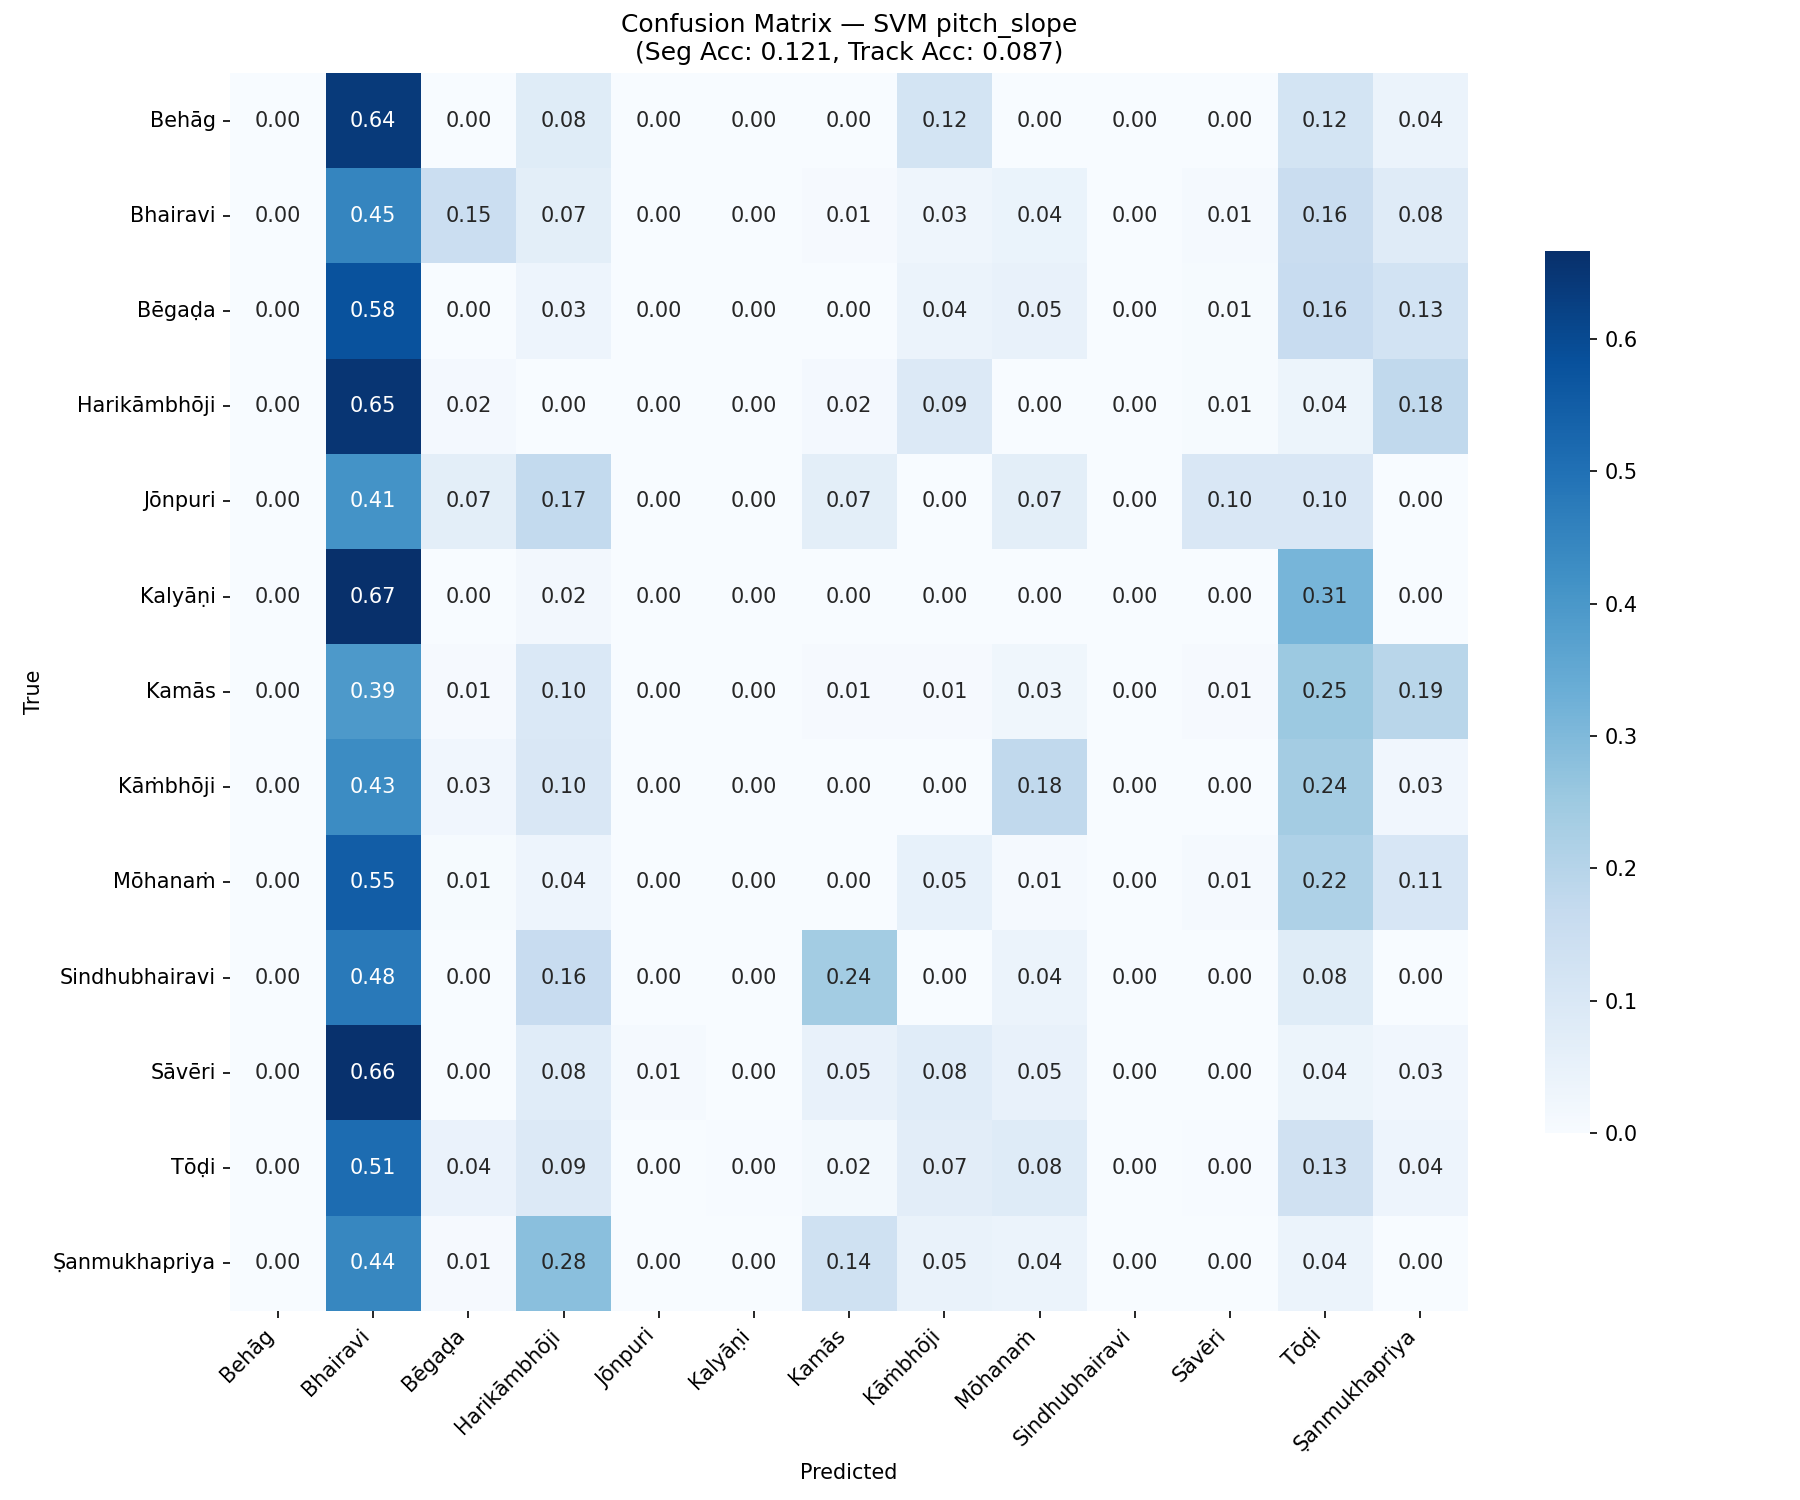
\includegraphics[width=\textwidth]{outputs/figures/classification/gamaka/cm_SVM_pitch_slope.png}
\caption{Pitch slope features}
\end{subfigure}
\hfill
\begin{subfigure}[b]{0.48\textwidth}
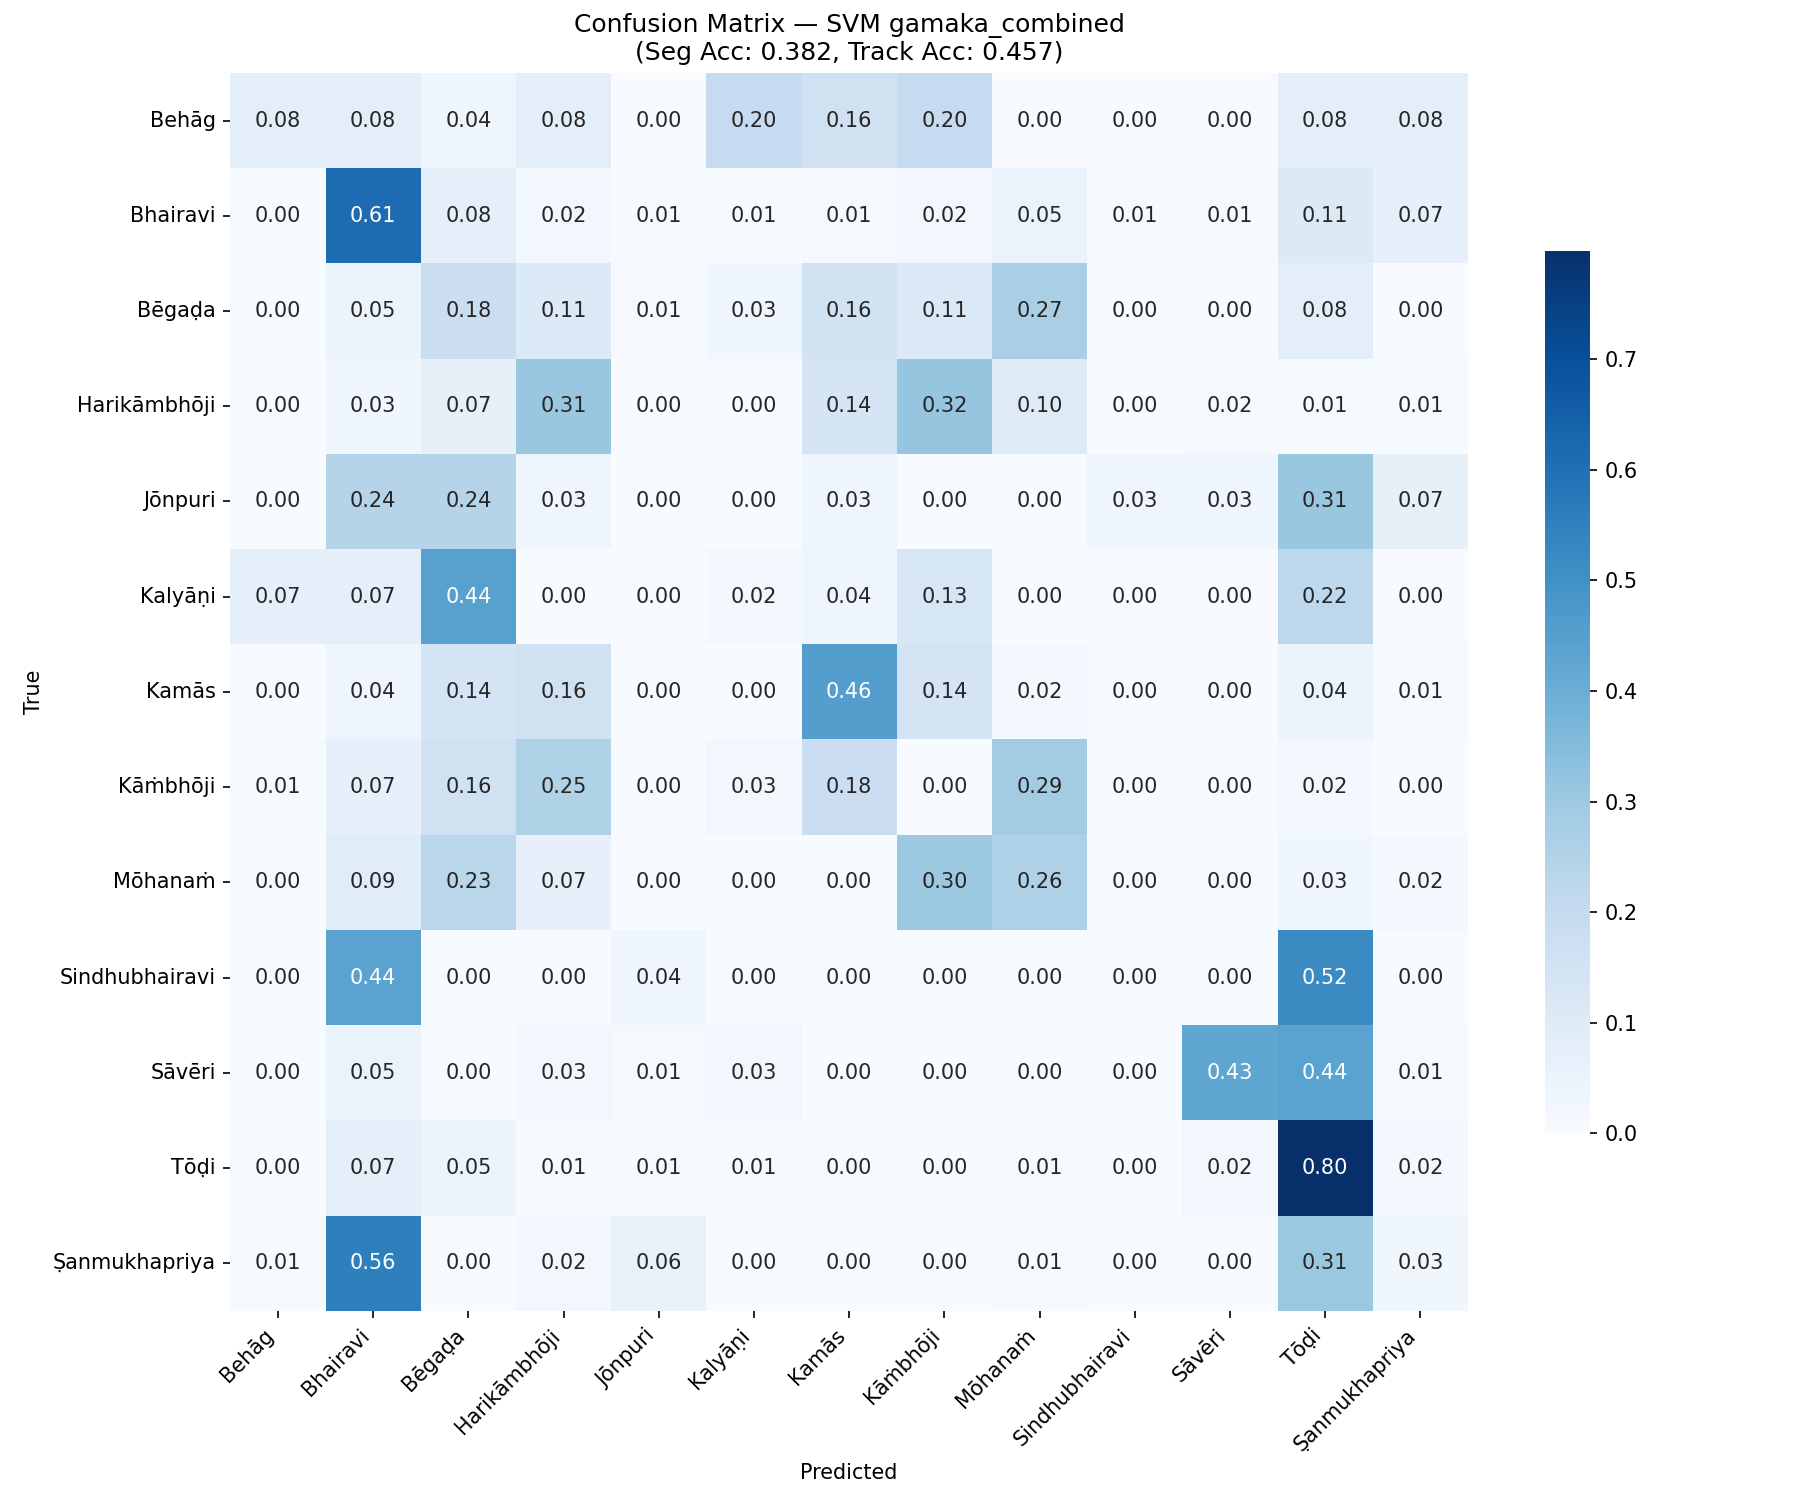
\includegraphics[width=\textwidth]{outputs/figures/classification/gamaka/cm_SVM_gamaka_combined.png}
\caption{Combined gamaka features}
\end{subfigure}
\caption{Gamaka experiment. Continuous pitch contour features do not improve classification --- pitch slope distributions are pan-\textit{raga} (all Carnatic music uses heavy ornamentation) rather than \textit{raga}-specific.}
\label{fig:app-cm-gamaka}
\end{figure}

\subsubsection{4-gram, Phrase Trigram, and Hierarchical}

\begin{figure}[H]
\centering
\begin{subfigure}[b]{0.48\textwidth}
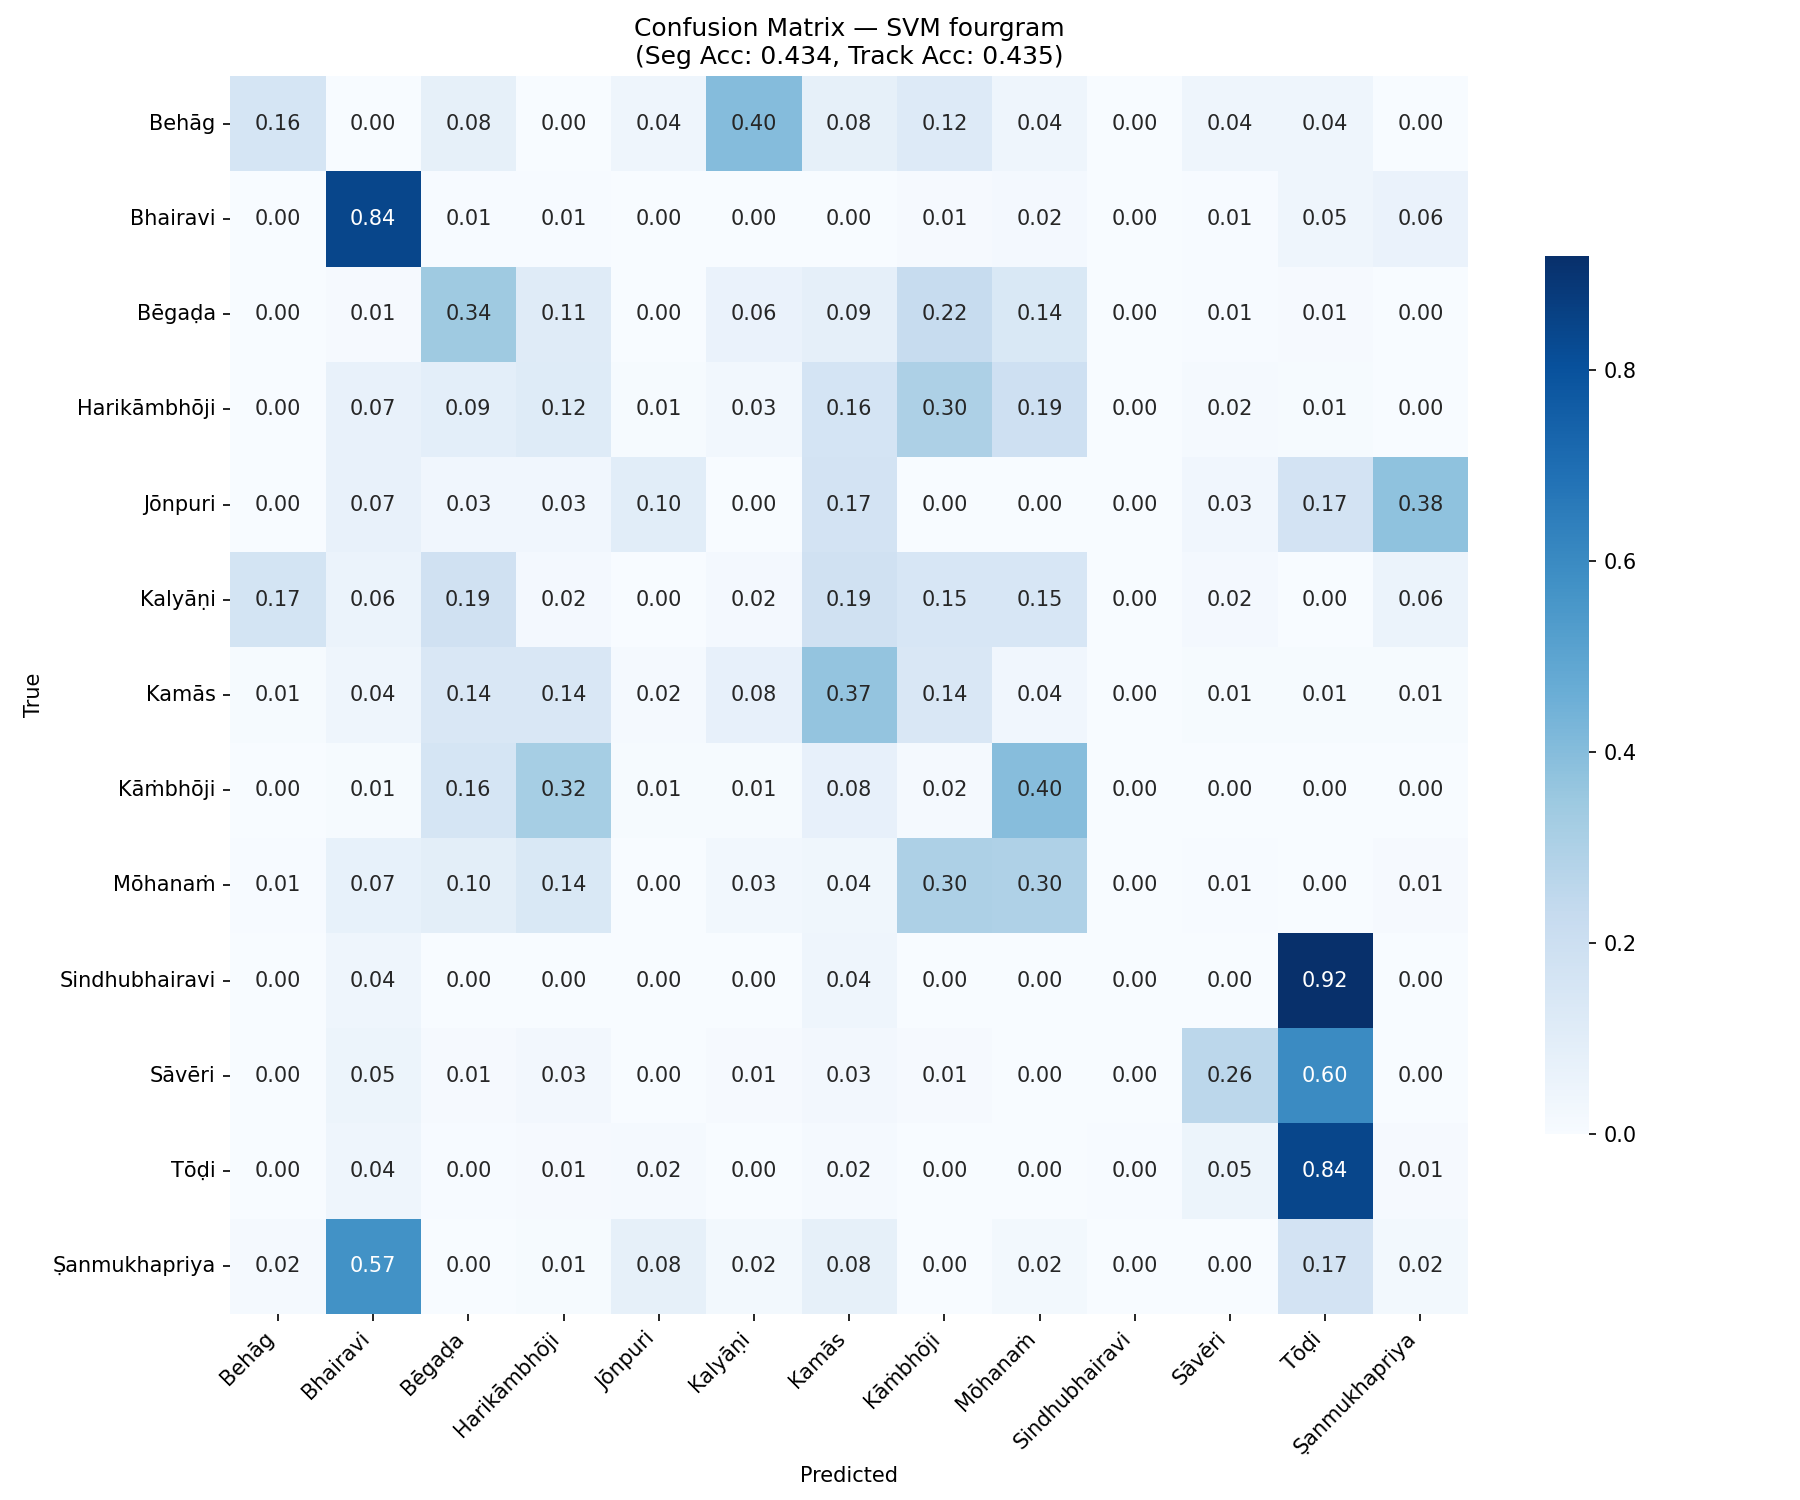
\includegraphics[width=\textwidth]{outputs/figures/classification/excl-est/cm_SVM_fourgram.png}
\caption{4-gram (200d) --- 43.5\% track acc, 38.8\% F1w}
\end{subfigure}
\hfill
\begin{subfigure}[b]{0.48\textwidth}
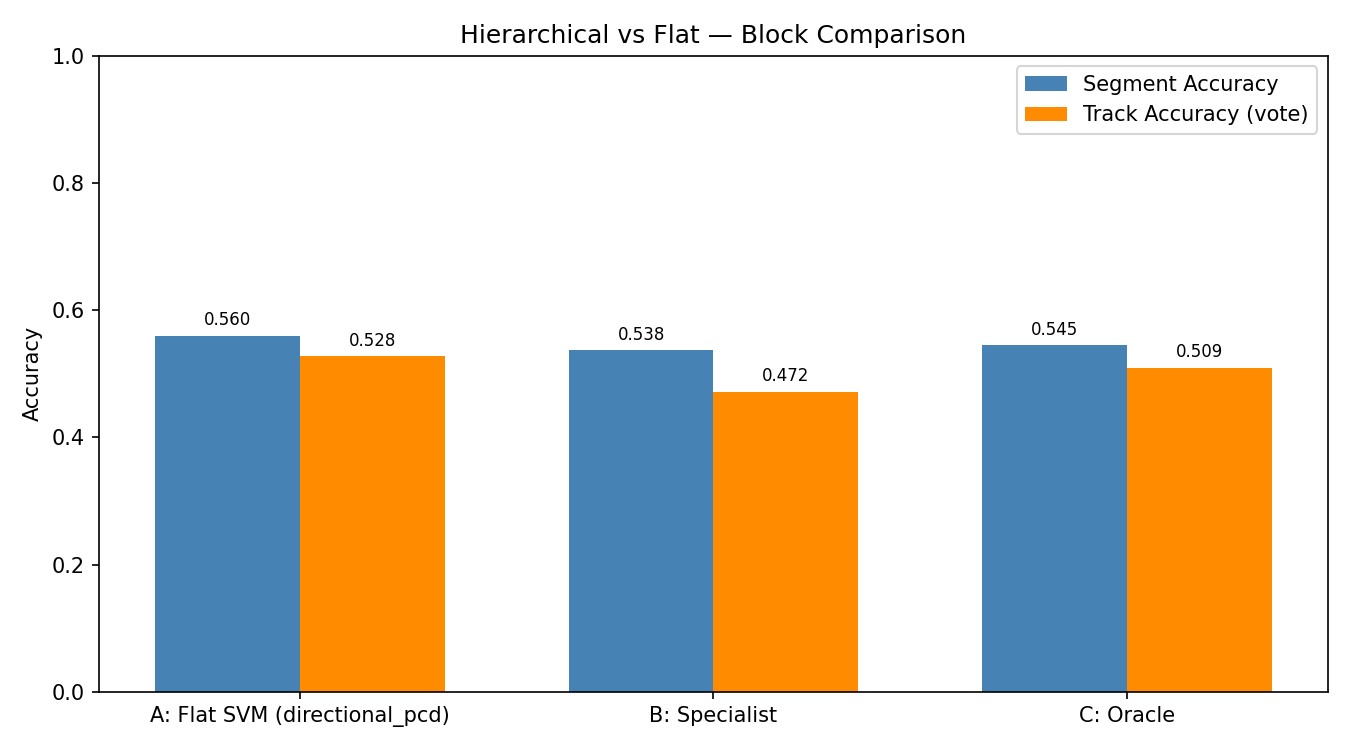
\includegraphics[width=\textwidth]{outputs/figures/hierarchical/block_comparison.png}
\caption{Hierarchical vs flat comparison}
\end{subfigure}
\caption{4-grams (top-200 vocabulary): underperforms trigrams despite identical dimensionality, confirming longer n-grams are too sparse with ${\sim}1{,}600$ training segments. Hierarchical: flat baseline matches or exceeds hierarchy because 60.7\% of errors are within-family (where L1 routing cannot help).}
\label{fig:app-cm-negative}
\end{figure}

\begin{figure}[H]
\centering
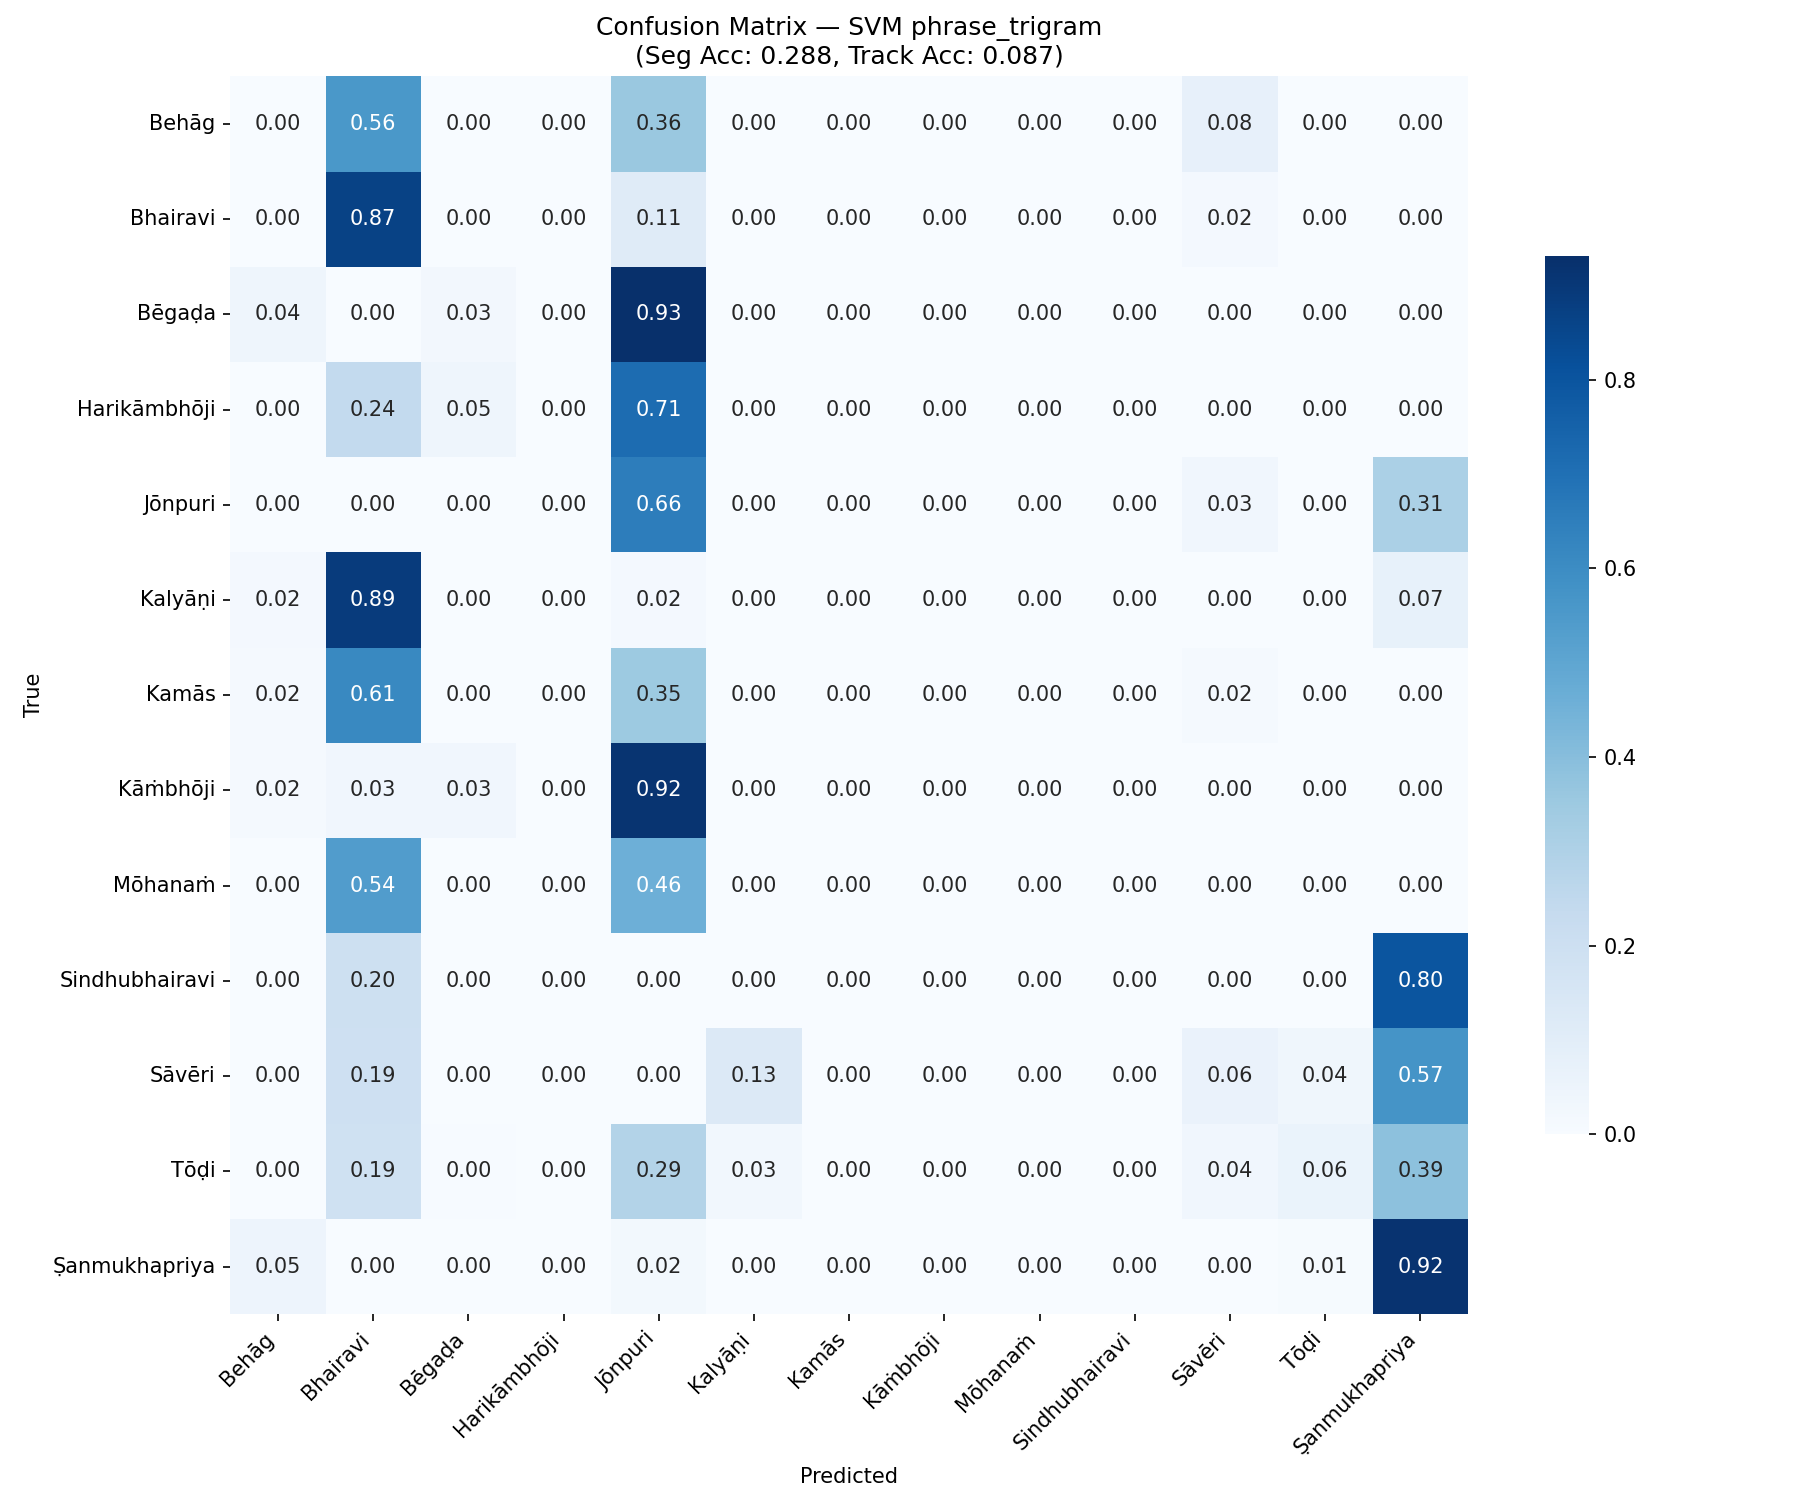
\includegraphics[width=0.55\textwidth]{outputs/figures/classification/excl-est/cm_SVM_phrase_trigram.png}
\caption{Phrase-aware trigram (200d) --- 8.7\% track acc, 2.8\% F1w. Segmenting the token stream at silence/glide boundaries before computing trigrams collapses performance to below chance. The silence/glide boundaries that phrase segmentation discards are themselves informative for \textit{raga} identity.}
\label{fig:app-cm-phrase-trigram}
\end{figure}

\subsection{Tonic Source Ablation: Full Estimated Tonic (All Tracks)}
\label{sec:app-est-all}

The table below shows classification results when \textbf{all tracks} are included using estimated tonic (no bad-tonic exclusion). Comparison with the primary results (bad-tonic excluded) quantifies the downstream impact of tonic estimation errors.

\begin{table}[H]
\centering
\caption{Classification results with estimated tonic, all tracks included (14 \textit{ragas}, 53 tracks, 2,107 segments). Compare with the primary results table in the main report (bad-tonic excluded) to see the downstream impact of tonic estimation failures.}
\label{tab:app-est-all}
\small
\begin{tabular}{lrrrr}
\toprule
\textbf{Model} & \textbf{Seg Acc} & \textbf{Seg F1w} & \textbf{Trk Acc} & \textbf{Trk F1w} \\
\midrule
SVM trigram\_dwell (216d)        & 43.38\% & 41.46\% & 56.60\% & 56.21\% \\
SVM trigram (200d)               & 42.43\% & 40.72\% & 50.94\% & 50.86\% \\
SVM directional\_pcd (408d)     & 42.29\% & 39.83\% & 52.83\% & 49.33\% \\
SVM directional\_full (418d)    & 41.72\% & 39.32\% & 52.83\% & 47.91\% \\
SVM pcd\_trigram (320d)          & 42.15\% & 39.71\% & 47.17\% & 44.87\% \\
SVM pcd\_trigram\_aux (330d)    & 41.29\% & 38.95\% & 49.06\% & 46.69\% \\
SVM dwell\_vadi (16d)            & 40.44\% & 37.83\% & 50.94\% & 45.21\% \\
SVM pcd (120d)                   & 37.07\% & 34.63\% & 50.94\% & 47.75\% \\
SVM fourgram (200d)              & 36.97\% & 35.10\% & 43.40\% & 41.31\% \\
Fusion (pcd+tri+tri\_dwell)     & 44.19\% & 41.31\% & 56.60\% & 55.24\% \\
LSTM swara\_seq                  & 36.73\% & 34.81\% & 43.40\% & 39.69\% \\
SVM phrase\_trigram (200d)       & 21.59\% & 17.93\% & 11.32\% &  5.04\% \\
SVM mfcc (58d)                   & 11.91\% &  3.95\% &  9.43\% &  3.45\% \\
\bottomrule
\end{tabular}
\end{table}

Key observations: (1) all models drop substantially compared to the bad-tonic-excluded condition, confirming that tonic estimation is the pipeline's primary bottleneck; (2) the ranking of feature sets is largely preserved: trigram\_dwell and fusion remain top performers; (3) phrase\_trigram collapses to 11.3\% track accuracy (below random), confirming the negative result from the main report; (4) MFCC remains near chance (9.4\%), consistent with H2 across conditions.

\subsection{Tonic Source Ablation: Ground-Truth Tonic}
\label{sec:app-gt}

The table below shows classification results when \textbf{ground-truth tonic} values from the SARAGA metadata are used instead of estimated tonic. This represents an upper bound on performance achievable if tonic estimation were perfect.

\begin{table}[H]
\centering
\caption{Classification results with ground-truth tonic (13 \textit{ragas}, 53 tracks). Compare with the estimated-tonic results to isolate the impact of tonic estimation errors on downstream classification.}
\label{tab:app-gt}
\small
\begin{tabular}{lrrrr}
\toprule
\textbf{Model} & \textbf{Seg Acc} & \textbf{Seg F1w} & \textbf{Trk Acc} & \textbf{Trk F1w} \\
\midrule
SVM trigram\_dwell (216d)        & 60.18\% & 59.50\% & 58.49\% & 54.90\% \\
SVM trigram (200d)               & 57.95\% & 57.34\% & 56.60\% & 51.81\% \\
SVM directional\_pcd (408d)     & 56.00\% & 53.56\% & 52.83\% & 49.08\% \\
SVM directional\_full (418d)    & 55.10\% & 52.74\% & 50.94\% & 47.80\% \\
SVM pcd\_trigram (320d)          & 56.76\% & 55.14\% & 49.06\% & 45.71\% \\
SVM pcd\_trigram\_aux (330d)    & 55.86\% & 54.38\% & 50.94\% & 47.01\% \\
SVM dwell\_vadi (16d)            & 52.97\% & 53.03\% & 52.83\% & 52.70\% \\
SVM pcd (120d)                   & 50.59\% & 49.47\% & 45.28\% & 40.25\% \\
SVM fourgram (200d)              & 49.03\% & 48.91\% & 45.28\% & 42.13\% \\
Fusion (pcd+tri+tri\_dwell)     & 59.09\% & 57.82\% & 52.83\% & 49.31\% \\
LSTM swara\_seq                  & 45.94\% & 45.15\% & 41.51\% & 39.44\% \\
SVM phrase\_trigram (200d)       & 17.89\% & 17.07\% &  9.43\% &  4.31\% \\
SVM mfcc (58d)                   & 11.91\% &  3.95\% &  9.43\% &  3.45\% \\
\bottomrule
\end{tabular}
\end{table}

Key observations: (1) segment-level accuracy improves substantially with ground-truth tonic (trigram\_dwell: 60.2\% vs 52.8\% excl-est), confirming tonic quality is the primary bottleneck; (2) surprisingly, track-level accuracy for dwell\_vadi is \textit{lower} with ground truth (52.8\%) than with estimated tonic excluding bad tracks (69.6\%) --- this is because the GT condition includes all 53 tracks (including difficult ones that were excluded in excl-est), while excl-est retains only 46 easier tracks; (3) MFCC remains at chance (9.4\%), confirming H2 is robust across all tonic conditions.

% ══════════════════════════════════════════════════════════
\section{Experiments}
% ══════════════════════════════════════════════════════════

\subsection{HPSS Tonic Estimation}

Harmonic-Percussive Source Separation (HPSS) via librosa was tested as a pre-processing step for tonic estimation. The hypothesis was that isolating the harmonic component would improve pitch histogram clarity by removing percussive transients. Results showed no improvement over running CREPE on the original mixture; CREPE's neural pitch tracker is already robust to percussive interference.

\subsection{Demucs Source Separation}

Deep source separation using Meta's Demucs (HTDemucs model) was tested to extract clean vocals before pitch extraction. While Demucs successfully isolates vocals, the resulting tonic estimates did not improve over the mixture baseline; the computational cost (${\sim}10\times$ slower) is not justified for this pipeline.

\subsection{Hindustani Cross-Tradition Pilot}

As a generalisability probe, the pipeline was applied to 10 tracks from the SARAGA Hindustani dataset (5 raags).

\begin{figure}[H]
\centering
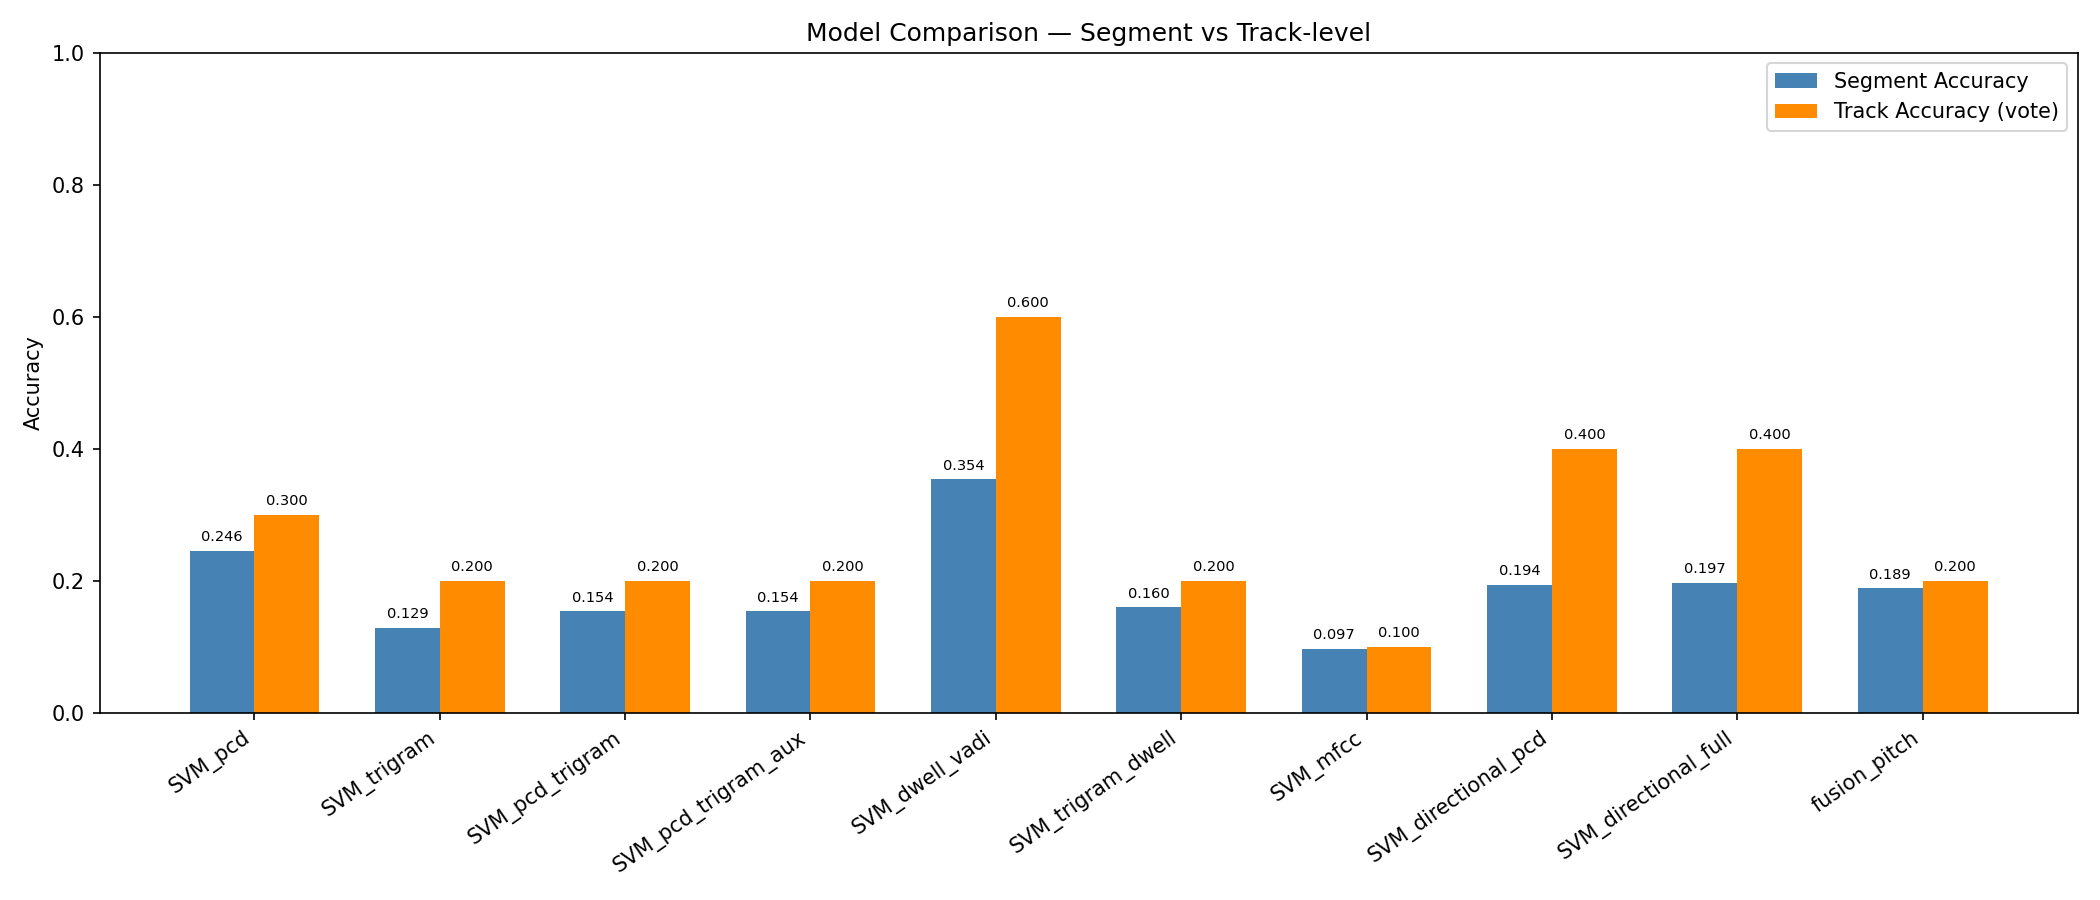
\includegraphics[width=0.75\textwidth]{outputs/hindustani/figures/classification/model_comparison.png}
\caption{Hindustani model comparison (10 tracks). Feature-importance flip: dwell\_v\=adi dominates while trigrams collapse --- consistent with Hindustani music being emphasis-driven rather than phrase-driven.}
\label{fig:app-hindustani-comparison}
\end{figure}

\begin{figure}[H]
\centering
\begin{subfigure}[b]{0.48\textwidth}
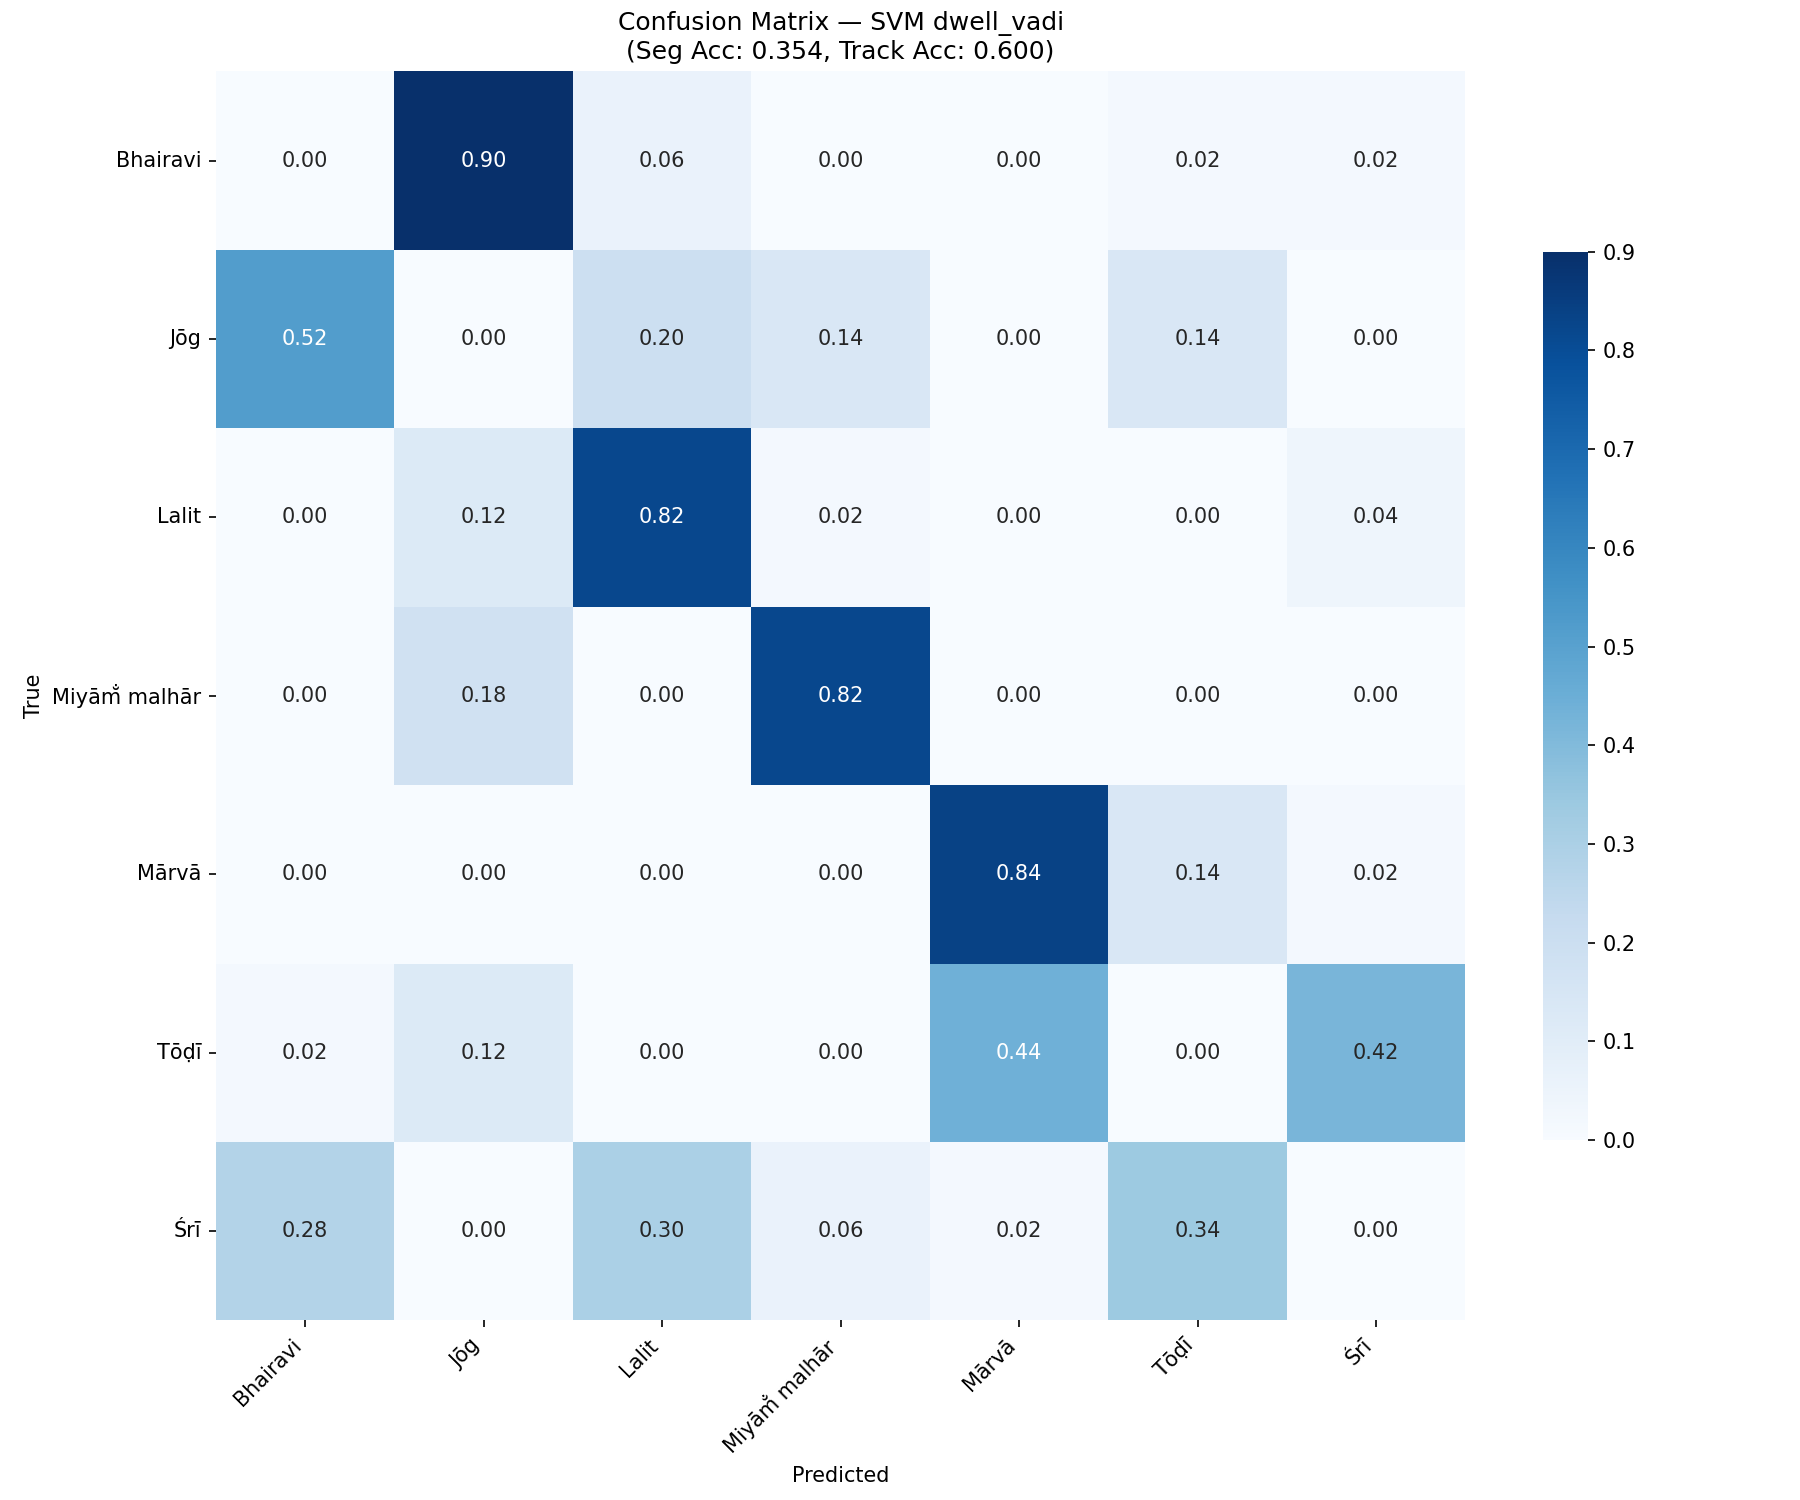
\includegraphics[width=\textwidth]{outputs/hindustani/figures/classification/cm_SVM_dwell_vadi.png}
\caption{Hindustani dwell\_v\=adi}
\end{subfigure}
\hfill
\begin{subfigure}[b]{0.48\textwidth}
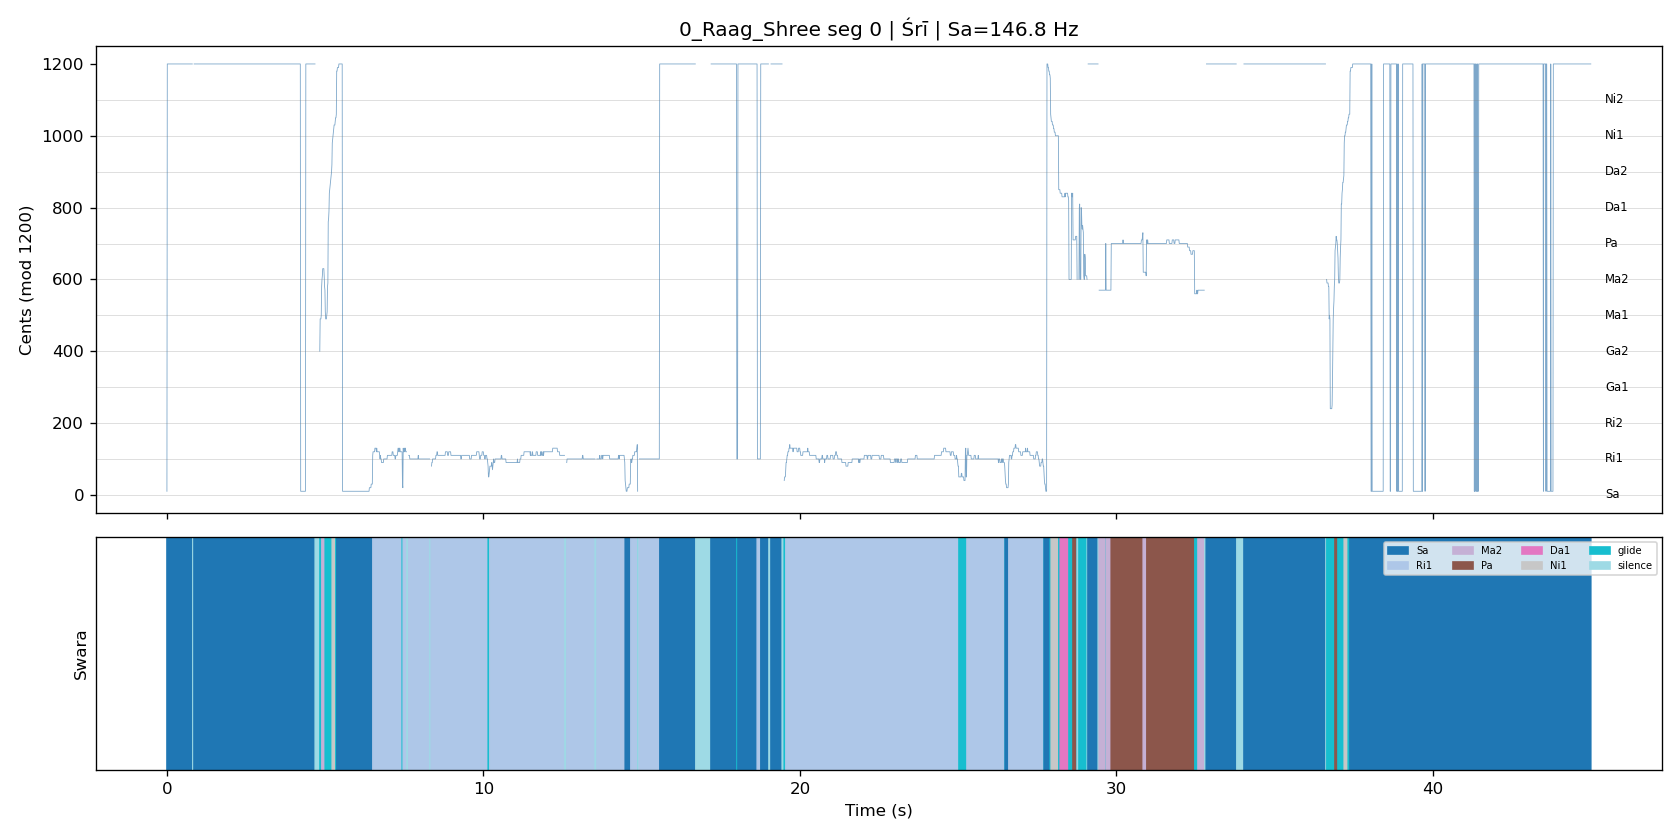
\includegraphics[width=\textwidth]{outputs/hindustani/figures/swara_debug/0_Raag_Shree__00000_swara.png}
\caption{Hindustani swara mapping: Raag Shree}
\end{subfigure}
\caption{Hindustani results: dwell\_v\=adi confusion matrix and swara mapping, demonstrating the pipeline operating on a different tradition.}
\label{fig:app-hindustani-detail}
\end{figure}

% ══════════════════════════════════════════════════════════
% \section{Repository References}
% ══════════════════════════════════════════════════════════
%
% The table below maps each figure in this appendix to its image file path in the repository. All paths are relative to the repository root.
%
% \begingroup
% \small
% \newcommand{\fp}[1]{\texttt{\seqsplit{#1}}}
% \begin{longtable}{@{}p{0.30\textwidth}p{0.65\textwidth}@{}}
% \toprule
% \textbf{Figure} & \textbf{Image Path} \\
% \midrule
% \endhead
% ... (Repository references table commented out)
% \bottomrule
% \end{longtable}
% \endgroup

\end{document}
